%To be used with Bibtex files
%May 2021 - This template was prepared by Dorothea F. Brosius of the
%Institute for Electronics and Applied Physics, University of Maryland, College Park, MD

%The template was last updated in May 2021
%Thesis Main Page used with thesis.sty based on the
%University of Maryland Electronic Thesis and Dissertation (ETD) Style Guide (2017)
% August 2017 (TOC contents linked in blue in pdf file) - DFB

% Select the version that fits how you are making this LaTeX document (its driver).
% The first two are the most likely ones to be needed.

 \newcommand{\mydriver}{pdflatex} %Making a PDF directly using pdflatex.
%\newcommand{\mydriver}{dvipdfmx} %Making a DVI and converting that to PDF using dvipdfmx.
%\newcommand{\mydriver}{dvipdfm} %Making a DVI and converting that to PDF using dvipdfm.
%\newcommand{\mydriver}{dvips} %Making a DVI and converting that to PS using dvips (may later be converted to PDF).
%\newcommand{\mydriver}{dvipsone} %Making a DVI and converting that to PS using dvipsone (may later be converted to PDF).
%\newcommand{\mydriver}{ps2pdf} %Same as the one for dvips except it is compatible with Ghostscript's PDF writer.


\documentclass[12pt,\mydriver]{thesis}  %12pt is larger than 11pt

\usepackage{titlesec}
   \titleformat{\chapter}
      {\normalfont\large}{Chapter \thechapter:}{1em}{}
\usepackage{times}
\usepackage{babel}
\usepackage{graphicx}
\usepackage{cite}
\usepackage{lscape}
\usepackage{indentfirst}
\usepackage{latexsym}
\usepackage{multirow}
\usepackage{epstopdf}
\usepackage{tabls}
\usepackage{wrapfig}
\usepackage{slashbox}
\usepackage{subeqn}
%\usepackage{subfigure}
%\usepackage{floatrow}
\usepackage{longtable}
\usepackage{supertabular}
%\usepackage[onehalfspacing]{setspace} %used for footnote spacing
\usepackage[table]{xcolor}
\usepackage{setspace}

%hyperref
\usepackage[colorlinks=true,urlcolor=black,linkcolor=blue,citecolor=blue]{hyperref}

\usepackage{tocloft,calc}
\renewcommand{\cftchapaftersnum}{:\ }
\renewcommand{\cftchappresnum}{\chaptername\space}
\setlength{\cftchapnumwidth}{\widthof{\textbf{Appendix\ }}}
\makeatletter
\g@addto@macro\appendix{%
  \addtocontents{toc}{%
    \protect\renewcommand{\protect\cftchappresnum}{\appendixname\space}%
  }%
}

\newcommand{\tbsp}{\rule{0pt}{18pt}} %used to get a vertical distance after \hline
\renewcommand{\baselinestretch}{2}
\setlength{\textwidth}{5.9in}
\setlength{\textheight}{9in}
\setlength{\topmargin}{-.50in}
%\setlength{\topmargin}{0in}    %use this setting if the printer makes the the top margin 1/2 inch instead of 1 inch
\setlength{\oddsidemargin}{.55in}
\setlength{\parindent}{.4in}
\pagestyle{empty}

\begin{document}
\pagestyle{empty}
%Abstract Page

\hbox{\ }

\renewcommand{\baselinestretch}{1}
\small \normalsize

\begin{center}
\large{{ABSTRACT}}

\vspace{3em}

\end{center}
\hspace{-.15in}
\begin{tabular}{ll}
Title of Dissertation:    & {\large  OPTIMIZING THE ACCURACY OF }\\
&                     {\large  LIGHTWEIGHT METHODS FOR SHORT READ} \\
&                     {\large  ALIGNMENT AND QUANTIFICATION} \\
\ \\
&                          {\large  Mohsen Zakeri} \\
&                           {\large Doctor of Philosophy, 2021} \\
\ \\
Dissertation Directed by: & {\large  Professor Rob Patro} \\
&               {\large  Department of Physics } \\
\end{tabular}

\vspace{3em}

\renewcommand{\baselinestretch}{2}
\large \normalsize

The analysis of the high throughput sequencing (HTS) data includes 
a number of involved computational steps, ranging from the assembly 
of the reference sequences, mapping or alignment of the reads to 
existing or assembled sequences, estimating the abundance of 
sequenced molecules, performing differential or comparative 
analysis between samples, and even inferring dynamics of interest 
from snapshot data. Many methods have been developed for these 
different tasks that provide different trade-offs in terms of 
accuracy and speed, because precision typically comes at the 
expense of sacrificing speed and vice versa. Throughout this 
work, I review different aspects of the available methods for 
alignment and quantification steps of RNA-seq data. Furthermore, 
I explore finding a reasonable balance between these competing 
goals to introduce methods which are designed to be almost as 
good as the most accurate approaches, while being as fast as the 
methods that focus on speed.

Alignment or mapping of the sequencing reads to the known reference 
sequences is a challenging computational step in the pipeline because 
of the large size of sample data. A typical RNA-seq sample often consists 
of 10s of millions of paired-end reads which should be queried against the 
large number of reference sequences to find the most similar reference substrings 
under some notion of edit distance. Therefore, the aligners index the reference 
sequences to accelerate the search procedure. Furthermore, recent quantification 
methods, introduced the concept of lightweight alignment in order to accelerate 
the mapping step, and therefore, the whole quantification pipeline. I collabrated 
with my colleagues to explore some of the shortcomings of the lightweight alignments, 
and to try to address those with a new approach called the selective alignment. 
Moreover, we introduce a new aligner, Puffaligner, which benefits from the indexing 
approach introduced by the Pufferfish index and also the idea of selective-alignment 
to produce accurate alignments in a short time compared to other popular aligners.

I have also explored the shortcomings of the approximate generative model used in the 
fast RNA-seq quantifiers. In these methods, fragments (reads) are grouped together 
into equivalence classes which are sets of sequenced fragments for which all the 
fragments are compatible with a specific set of reference sequences. Therefore, in 
the approximate models, all the fragments in each group are treated as identical, 
which factorizes the likelihood function being optimized and increases the speed of 
the optimization step. I have explored how this factorization affects the accuracy of 
abundance estimates, and propose a new factorization approach for approximating the 
likelihood which demonstrates higher fidelity to the exact model.

%Finally, I propose the possible path forward for increasing the accuracy of 
%abundance estimation tools in the cases where there are anomalies in transcript 
%coverages which could lead to the detection of unannoated transcripts. Also, 
%I will investigate if representing single cell expression matrices in terms of 
%equivalence classes, rather than the gene counts, increases the accuracy or 
%robustness of the downstream analysis of the single cell pipelines, such as 
%dimensionality reduction and cell clustering. %(must be first, required, non-numbered)
%Titlepage

\thispagestyle{empty}
\hbox{\ }
\vspace{1in}
\renewcommand{\baselinestretch}{1}
\small\normalsize
\begin{center}

\large{{Optimizing the accuracy of lightweight methods 
for short read alignment and quantification}}\\
\ \\
\ \\
\large{by} \\
\ \\
\large{Mohsen Zakeri}%Your full name as it appears in University records.
\ \\
\ \\
\ \\
\ \\
\normalsize
Dissertation submitted to the Faculty of the Graduate School of the \\
University of Maryland, College Park in partial fulfillment \\
of the requirements for the degree of \\
Doctor of Philosophy \\
2021
\end{center}

\vspace{7.5em}

\noindent Advisory Committee: \\
Professor Rob Patro, Chair/Advisor \\
Professor Mihai Pop \\
Professor John Dickerson \\
Professor Erin Molloy \\
Professor Michael Cummings, Dean's representative
 %(must follow Abstract, required, non-numbered)
%Copyright

\thispagestyle{empty}
\hbox{\ }

\vfill
\renewcommand{\baselinestretch}{1}
\small\normalsize

\vspace{.5in}

\begin{center}
\large{\copyright \hbox{ }Copyright by\\
Mohsen Zakeri  %Type your name as it appears in University records
\\
2021}
\end{center}

\vfill

\newpage 
 %(highly recommended, non-numbered)

%Pages from this point start at lower-case Roman number ii)
\pagestyle{plain} \pagenumbering{roman} \setcounter{page}{2}
\addcontentsline{toc}{chapter}{Preface}
%Preface
\pagestyle{plain}\pagenumbering{roman} \setcounter{page}{2}
\renewcommand{\baselinestretch}{2}
\small\normalsize
\hbox{\ }

\vspace{.5in}

\begin{center}
\large{Preface}
\end{center}


If needed.
  %(if present, start at lower-case Roman number ii)
\addcontentsline{toc}{chapter}{Foreword}
%Foreword

\renewcommand{\baselinestretch}{2}
\small\normalsize
\hbox{\ }
 
\vspace{.5in}

\begin{center}
\large{Foreword} 
\end{center} 

If needed.
 %(if present, lower-case Roman)
\addcontentsline{toc}{chapter}{Dedication}
%Dedication

\renewcommand{\baselinestretch}{2}
\small\normalsize
\hbox{\ }
 
\vspace{.5in}

\begin{center}
\large{Dedication}
\end{center} 

To Zahra and Mohammad Sadegh who are always there for me. %(if present, lower-case Roman)
\addcontentsline{toc}{chapter}{Acknowledgements}
%Acknowledgments

\renewcommand{\baselinestretch}{2}
\small\normalsize
\hbox{\ }
 
\vspace{.5in}

\begin{center}
\large{Acknowledgments} 
\end{center} 

\vspace{1ex}

I owe my gratitude to all the people who have made this thesis possible and because of whom my graduate experience has been one that I will cherish forever.

First and foremost I'd like to thank my advisor, Professor Rajarshi Roy for giving me an invaluable opportunity to work on challenging and extremely interesting projects over the past four years. He has always made himself available for help and advice and there has never been an occasion when I've knocked on his door and he hasn't given me time. It has been a pleasure to work with and learn from such an extraordinary individual.

I would also like to thank my co-advisor, Dr. Parvez Guzdar. Without his extraordinary theoretical ideas and computational expertise, this thesis would have been a distant dream. Thanks are due to Professor Robert Gammon, Professor Edward Ott and Professor Thomas Antonsen for agreeing to serve on my thesis committee and for sparing their invaluable time reviewing the manuscript.

My colleagues at the nonlinear optics laboratory have enriched my graduate life in many ways and deserve a special mention. David DeShazer helped me start-off by rewriting the basic simulation code in a user-friendly format. Christian Silva provided help by setting up the GRENOUILLE apparatus and performing some of the simulations. My interaction with  Rohit Tripathi, Ryan McAllister, Vasily Dronov, Min-Young Kim, Elizabeth Rogers, William Ray, Jordi Garcia Ojalvo, Riccardo Meucci, Atsushi Uchida, and Fabian Rogister has been very fruitful. I'd also like to thank Wing-Shun Lam and Benjamin Zeff for providing the LaTex style files for writing this thesis.

I would also like to acknowledge help and support from some of the staff members. Donald Martin's technical help is highly appreciated, as is the computer hardware support from Edward Condon, LaTex and software help from Dorothea Brosius and purchasing help from Nancy Boone.

I owe my deepest thanks to my family - my mother and father who have always stood by me and guided me through my career, and have pulled me through against impossible odds at times. Words cannot express the gratitude I owe them. I would also like to thank Dr. Mohan Advani, Dr. Vasudeo Paralikar and Dr. Vinod Chaugule who are like family members to me.

My housemates at my place of residence have been a crucial factor in my finishing smoothly. I'd like to express my gratitude to Sivasankar Pandeti, Jayakumar Patil, Amit Trehan and Punyaslok Purakayastha for their friendship and support.

I would like to acknowledge financial support from the Office of Naval Research (ONR), Physics, for all the projects discussed herein.

It is impossible to remember all, and I apologize to those I've inadvertently left out.

Lastly, thank you all and thank God!
 %(if present, lower-case Roman)
    \cleardoublepage
    \phantomsection
    \addcontentsline{toc}{chapter}{Table of Contents}
    \renewcommand{\contentsname}{Table of Contents}
\renewcommand{\baselinestretch}{1}
\small\normalsize
\tableofcontents %(required, lower-case Roman)
\newpage
\addcontentsline{toc}{chapter}{List of Tables}
    \renewcommand{\contentsname}{List of Tables}
\listoftables %(if present, lower-case Roman)
\newpage
\addcontentsline{toc}{chapter}{List of Figures}
    \renewcommand{\contentsname}{List of Figures}
\listoffigures %(if present, lower-case Roman)
\newpage
% LIST OF ABBREVIATIONS
\addcontentsline{toc}{chapter}{List of Abbreviations}
%List of Abbreviations


\renewcommand{\baselinestretch}{1}
\small\normalsize
\hbox{\ }

\vspace{.5in}

\begin{center}
\large{List of Abbreviations}
\end{center} 

\vspace{3pt}

\begin{supertabular}{ll}


\textbf{ARD} & \textbf{A}bsolute  \textbf{R}elative \textbf{D}ifference\\
%\textbf{BLAST} & \textbf{B}asic \textbf{L}ocal \textbf{A}lignment \textbf{S}earch \textbf{T}ool\\
\textbf{BWT} & \textbf{B}urrows-\textbf{W}heeler \textbf{T}ransform\\
\textbf{DP} & \textbf{D}ynamic-\textbf{P}rogram\\
\textbf{EM} & \textbf{E}xpectation \textbf{M}aximization\\
\textbf{HTS} & \textbf{H}igh \textbf{T}hroughput \textbf{S}equencing\\
\textbf{Indel} & \textbf{In}sertion (and) \textbf{D}eletion\\
\textbf{MARD} & \textbf{M}ean \textbf{A}bsolute  \textbf{R}elative \textbf{D}ifference\\
\textbf{MEM} & \textbf{M}aximal \textbf{E}xact \textbf{M}atch\\
\textbf{NGS} & \textbf{N}ext \textbf{G}eneration \textbf{S}equencing\\
\textbf{SA} & \textbf{S}uffix \textbf{A}rray\\
\textbf{SGS} & \textbf{S}econd \textbf{G}eneration \textbf{S}equencing\\
%\textbf{SIMD} & \textbf{S}ingle \textbf{I}nstruction \textbf{M}ultiple \textbf{D}ata\\
\textbf{SMEM} & \textbf{S}uper \textbf{M}aximal \textbf{E}xact \textbf{M}atch\\
\textbf{uni-MEM} & \textbf{U}nique \textbf{M}aximal \textbf{E}xact \textbf{M}atch\\
\textbf{VBEM} & \textbf{V}ariational \textbf{B}ayesian - \textbf{E}xpectation \textbf{M}aximization\\
    
% AAA & Antiaircraft artillery \\
% ABCCC & Airborne Battlefield Command and Control Center \\
% AEHF & Advanced Extremely High Frequency \\
% AGM & Air-to-ground guided missile \\
% AIT & Assembly, Integration, and Testing \\
% AOR & Area of Responsibility \\
% APAM & Anti-personnel, anti-material \\
% ASOC & Air Support Operations Center \\
% ATACM & Army Tactical Missile System \\
% ATO & Air Tasking Order \\
% AWACS & Airborne Warning and Control System \\
% \\
% BAT & Brilliant Ani-Armor Submunition \\
% BDA & Bomb-damage assessment  \\
% BFT & Blue Force Tracking \\
% BLOS & Beyond Line-of-Sight \\
% BMD & Ballistic Missile Defense \\
% \\
% C$^{3}$ & Command, Control, and Communications \\
% CAFMS & Computer-aided Force Management System \\
% CALCM & Conventional Air-Launched Cruise Missile \\
% CBU & Cluster Bomb Unit \\
% CCAFS & Cape Canaveral Air Force Station \\
% CENTAF & CENTCOM's Air Force component \\
% CENTCOM & U.S. Central Command \\
% CINC & Commander-in-Chief \\
% CONUS & Continental United States \\
% \\
% DAGR & Defense Advanced GPS Reciever \\
% DMA & Defense Mapping Agency \\
% DOD & Department of Defense \\
% DOP & Dilution of Precision \\
% DOT & Department of Transportation \\
% DSMAC & Digital Scene Mapping Area Correlator \\
% \\
% EFOG-M & Enhanced Fiber Optic Guided Missile \\
% \\
% FAA & Federal Aviation Administration \\
% FLIR & Forward-looking infrared \\
% \\
% GAM & Global Positioning System Aided Munition \\
% GPS & Global Positioning System \\
% GWAPS & Gulf War Air Power Survey \\
% \\
% HARM & High-Speed Antiradiation Missile \\
% HEO & Highly Elliptical Orbit \\
% \\
% IADS & Integrated Air Defense System \\
% ICBM & Inter-Continental Ballistic Missile \\
% INS & Inertial navigation system \\
% IIR & Imaging infrared \\
% IR & Infrared \\
% ISR & Intelligence, Surveillance, and Reconnaissance \\
% \\
% JDAM & Joint Direct Attack Munition \\
% JFC & Joint Force Commander \\
% JSOW & Joint Standoff Weapon \\
% \\
% LANTIRN & Low-Altitude Navigation and Targeting Infrared for Night System \\
% LEO & Low Earth Orbit \\
% LGB & Laser-guided bomb \\
% \\
% MAJIC & Microsatellte Area-Wide Joint Information Communication \\
% MARCENT & CENTCOM's Marine component \\
% MARS & Mid-Atlantic Regional Spaceport \\
% MLRS & Multiple Launch Rocket System \\
% MUOS & Mobile User Objective System \\
% \\
% NASA & National Aeronautics and Space Administration \\
% NAVCENT & CENTCOM's Navy component \\
% NPOESS & National Polar-Orbiting Operational Environmental Satellite System \\
% \\
% ORS & Opertionally Responsive Space \\
% ORSO & Operationally Responsive Space Office \\
% \\
% PDOP & Position Dilution of Precision \\
% PGM & Precision-guided munition \\
% P$^{3}I$ & Preplanned Product Improvement \\
% PnP & Plug and Play \\
% PnPSat & Plug and Play Satellite \\
% PPS & Precise Positioning Service \\
% \\
% RCS & Radar cross section \\
% \\
% SA & Situational Awareness \\
% SADARM & Sense and Destroy Armor Munition \\
% SAM & Surface-to-air missile \\
% SAR & Synthetic aperture radar \\
% SBIRS & Space Based Infrared System \\
% SEAD & Suppression of enemy air defenses \\
% SFW & Sensor Fuzed Weapon \\
% SIGINT & Signal Intelligence \\
% SLAM & Standoff Land Attack Missile \\
% SLAM-ER & SLAM-Expanded Response \\
% SpaceX & Space Exploration Technologies Corporation \\
% SPS & Standard Positioning Service \\
% \\
% TACC & Tactical Air Control Center \\
% TACS & Tactical Air Control System \\
% TACP & Tactical Air Control Party \\
% TASM & Tomahawk Anti-Ship Missile \\
% TBIP & Tomahawk Baseline Improvement Program \\
% TERCOM & Terrain Contour Mapping \\
% TFR & Terrain-following radar \\
% TLAM & Tomahawk Land Attack Missile \\
% \\
% USAF & U.S. Air Force \\
% \\
% VAFB & Vandenberg Air Force Base \\
% \\
% WGS & Wideband Global SATCOM \\
%$\alpha$ & alpha \\
%$\beta$  & beta \\
%&  \\ 
%IREAP & Institute for Research in Electronics and Applied Physics \\
%NSA & National Security Agency
\end{supertabular}


\newpage
\setlength{\parskip}{0em}
\renewcommand{\baselinestretch}{2}
\small\normalsize

%Pages from this point start at Arabic numeral 1
\setcounter{page}{1}
\pagenumbering{arabic}
%Chapter 1

\renewcommand{\thechapter}{1}

%\chapter{Introduction}

\chapter{Introduction} % Main chapter title
\label{intro} % For referencing the chapter elsewhere, use \ref{Chapter1} 

Out of the four major biological macromolecules (proteins, carbohydrates, lipids 
and nucleic acids), nucleic acids carry the most significant information about 
the identity of each organism. Even within each organism, the different 
content of nucleic acids in different organs and cells, defines their main 
functions and characteristics, also known as phenotypes. There are four 
types of nucleic acids (\textbf{A}denine, \textbf{C}ytosine, 
\textbf{T}hymine(\textbf{U}racil), \textbf{G}uanine) which are 
the main components of the \textbf{D}eoxyribo\textbf{N}ucleic 
\textbf{A}cids (DNA) and \textbf{R}ibo\textbf{N}ucleic 
\textbf{A}cid (RNA) in living organisms (Archaea, Bacteria, and Eukarya). 
Each DNA or RNA molecule is formed by a sequence of the nucleic acids. 
While the DNA content of different organisms are distinct, the DNA molecules 
across all cells of each individual are almost identical. Even during 
the cell division, all the DNA molecules are duplicated and preserved 
in each new cell's nucleus in the form of chromosomes. On the other hand, 
there exists different types of RNA molecules in different cells of each 
organism, leading to their different functions. RNA molecules are created 
from specific regions of chromosomes, called genes, in a process called 
transcription. A gene is called expressed in a specific cell if it is 
transcribed to RNA molecules. Different genes being expressed in different 
cell types leads to their vastly various functions. The set of all the genes, 
and the set of all the RNA molecules present in a cell are called the genome 
and the transcriptome respectively.

The transcription of a gene is started by a specific protein called the RNA 
polymerase. This protein copies the sequence of nucleic acids from a gene into 
a new RNA-sequence, called the pre-mRNA. There are two main types of 
subsequences present in each pre-mRNA, introns (intragenic regions) and exons 
(expressed regions).The pre-mRNA molecules turn into the mRNA molecules after 
the intronic regions are spliced out.
Alternative splicing of the set of introns and exons generates various mRNA 
molecules from a single gene. The set of all mRNA molecules generated from a 
single gene are called the isoforms or transcripts of the gene. 
\Cref{fig:altsplice} shows how two different isoforms are generated 
from a single gene through alternative splicing.

Many technologies have been proposed for gathering information about 
the transcriptomic contents of an organism. RNA sequencing (RNA-seq) is a 
powerful sequencing technique, and has become very popular since its 
introduction~\citep{mortazavi}. In the RNA-seq protocols, RNA sequences are 
first fragmented into smaller pieces, then these fragments are amplified 
through the PCR process, and finally the set of amplified fragments are 
sequenced and read sequences are generated. If both ends (5' and 3') of the 
fragments are sequenced paired end reads will be generated, while single 
end reads are sequenced only from a single end of each fragment.
Transcriptome assembly, detecting novel isoforms, and measuring the 
expression level of any isoform in a sample, are some of the main 
important applications of RNA-seq data. Mapping or alignment of RNA-seq 
reads to the set of known references is one of the early computational 
steps in many of these applications. Throughout this section, some famous 
computational approaches proposed for this critical step are introduced.


The number of reads generated from each isoform of a gene depends on the 
gene's level of expression in the cell. Each gene consists of encoding 
segments called exons. Each transcript or isoform of a gene consists of 
a set of particular exons. To illustrate the alternative splicing, consider 
the example in~\cref{fig:altsplice} that shows two different isoforms of 
$gene_a$ which is a gene with three exons. Different splicing events can 
lead to new combinations of exons in each isoform, e.g., $t_1$ and $t_2$ 
are two isoforms generated from $gene_a$, each containing specific subset 
of exons of $gene_a$. While in rare cases, i.e., back-splicing, the order
of the exons can be changed in the isoforms, generally we expect to see the same
ordering of the exons in the isoforms as in the genes.
The number of reads mapping to specific exons and exon junctions
is proportional to the expression level of the isoforms containing those exons. 
As more copies of an isoform exist in the sample, more reads map to it.
According to sequence similarities in different genes or exons shared between different 
isoforms of a gene, a read may map to multiple isoforms in the transcriptome, 
this ambiguity makes abundance estimation challenging. An example of reads 
generated from different isoforms of a gene in RNA-seq experiments is displayed 
in~\cref{fig:altsplice}. In this example, green and blue reads suggest 
expressions of both $t_1$ and $t_2$, while red reads are only compatible 
with $t_1$. 

Reads spanning two different exons can be evidence for the splicing events, 
e.g., the green-blue read in~\cref{fig:altsplice} spans the red and green 
exons which suggest the existence of an isoform containing these two exons 
next to each other, i.e., $t_2$. In this example, $t_1$ and $t_2$ are the 
known isoforms (also called transcripts) of the gene $gene_a$. In an RNA-seq 
experiment reads might be generated that do not map to any known isoforms of 
genes, e.g., the gray reads mapping to the intronic gray region of $gene_a$ 
in~\cref{fig:altsplice} or green-gray read that maps to the exon-intron 
junction. Presence of such reads could be evidence for discovering new exons 
or isoforms of $gene_a$, or preserved intronic regions in the isoforms (intron 
retention). Finding evidence for novel isoforms or intron retention events is 
an important advantage of RNA-seq assay over alternative sequencing techniques.

\begin{figure}
 \centering
 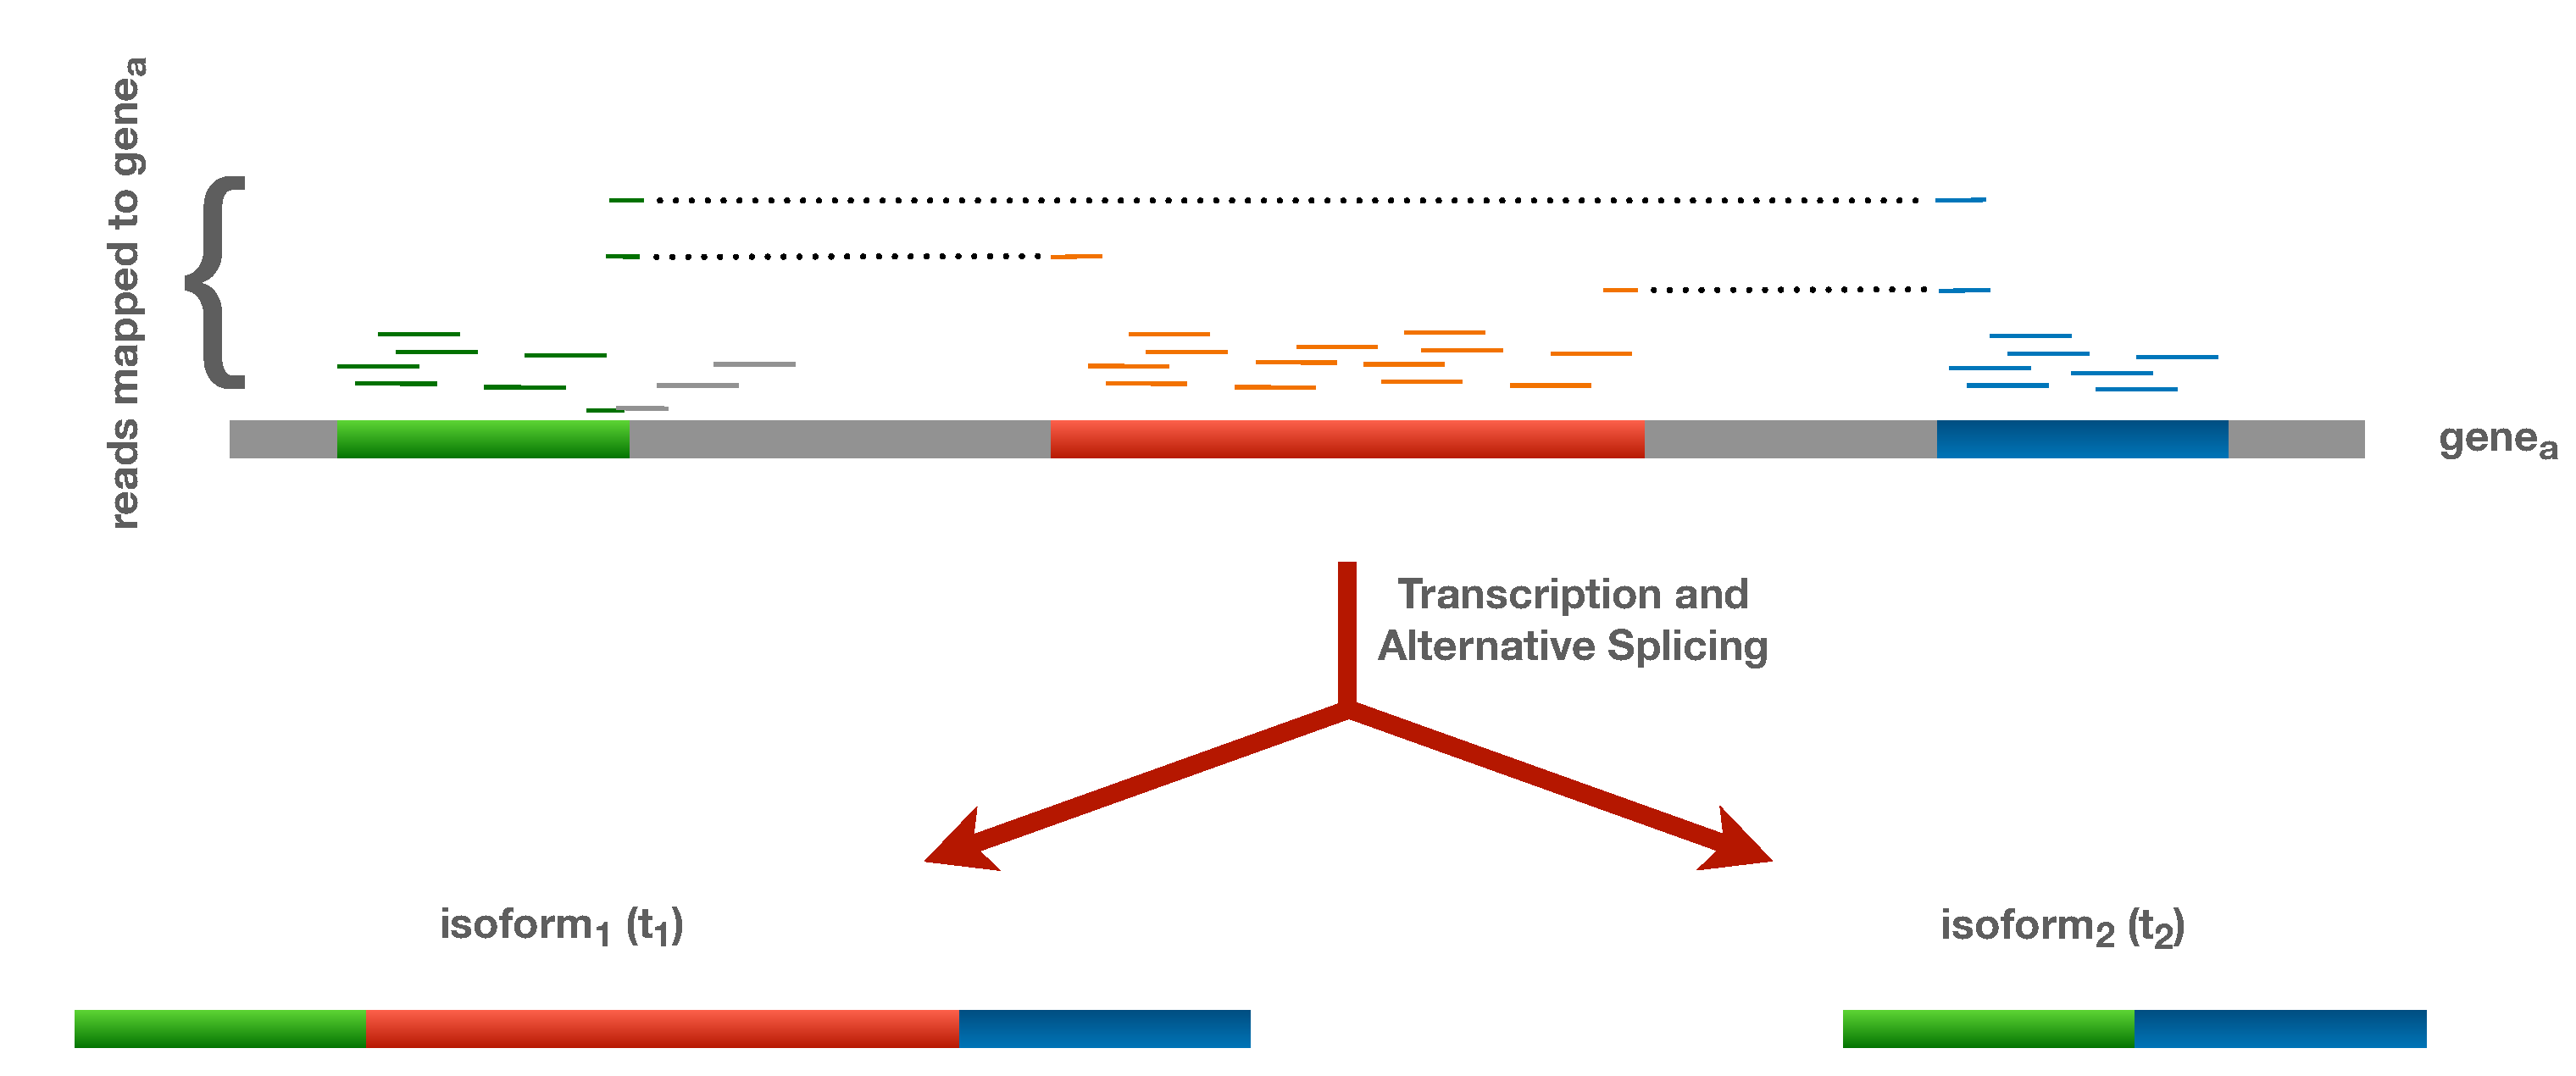
\includegraphics[width=0.95\columnwidth]{Figures/intro/alt-splice.pdf}
 \caption[Alternative splicing of genes]{An example of splicing events in 
 the gene $gene_a$, resulting in two transcripts $t_1$ and $t_2$. According 
 to sequence similarities the RNA-seq reads might be mapped to single or 
 multiple isoforms.}
  \label{fig:altsplice}
\end{figure}

In the following sections of this chapter I review the existing tools which 
are widely used for alignment (computing the edit distance of the reads to 
the reference sequences) and quantification (estimating the expression ratio 
of the isoforms) of RNA-seq samples. Both of these steps greatly affect the 
accuracy of the downstream analysis in RNA-seq pipelines~\citep{srivastava2019alignment}. 
Qunatification of RNA-seq data is a very challenging task due to a high degree of
multimapping~\citep{van2019rna}. Accurate RNA-seq abundance estimations are essential for detecting
differentially expressed genes and transcripts. It has been shown that 
disease-associated transcriptomic alterations can be studied with precise abundance estimation
at the transcript level~\citep{dick2020differential}.

In chapter 2, we present a fast mapping technique called \sla~\citep{selaln}. 
This technique is built alongside \qm to achieve a higher sensitivity that results in more 
accurate abundance estimates. Chapter 2 also introduces a new tool for 
computing alignment of DNA-seq and RNA-seq reads to known reference sequences. 
In chapter 3, an improved factorization of the quantification likelihood 
function is presented that maintains a high fidelity to the underlying 
data and will result in higher confidence for more fine grained analysis 
of transcripts. 
% In chapter 4 the future work for my PhD research will be 
% proposed which involves projects for improving the RNA-seq quantification 
% accuracy and utilizing the equivalence classes for downstream analysis of 
% single cell samples. 
% In chapter 4, we briefly discuss performing further analysis with our 
% proposed methods, such as achieving more robust estimates by using different 
%optimization techniques.

\section{Mapping RNA-seq reads to a known transcriptome}

Alignment is a crucial and expensive computational step in an RNA-seq analysis 
pipeline. The main goal of this step is to find, for each read, the region on 
the reference genome (or transcriptome) from which it is originally fragmented. 
The length of each short RNA-seq read is usually between 100 and 200 bases, 
while the length of the latest human genome is about three billion bases. The goal, 
for each read, is  to find a substring in the reference sequences that best 
matches the read. Often it is not possible to find an exact match for a read 
because of the variations present in the samples with respect to the reference 
sequences. The variations are divided into two main types, variations introduced 
by technical errors or the biological variations existing in each new sample. 
Therefore, the alignment procedure most of the time results in an inexact 
match for each read rather than a region which exactly matches the read. 
In order to find the most compatible regions in the reference sequences to 
each read, we should define the edit distance between two sequences.
%compatibility of two sequences. The compatibility is measured by 
The edit distance is proportional to the number of edits required to convert one sequence to the 
other one. Different types of edits, such as substitutions and insertions/deletions,  
are considered.% which are substitution, insertion and deletion. 
The sequence of edits can be shown in the form of \texttt{CIGAR} strings.
\texttt{CIGAR} strings are a sequence of operators to be applied in the first sequence
to be converted into the other one. 
The penalties assigned to each type of edit can be 
different and are usually configurable in most aligners. The sum of 
all the penalties is considered to be the edit distance between two sequences.
Therefore, we can define the alignment problem as finding the region on the 
reference with the minimum edit distance to each read. 
This can be achieved 
by classical algorithms, such as Smith-Waterman~\citep{smith1981identification}, 
in $O(n*m)$ time and $O(n*m)$ space, where $n$ and $m$ are the length of the 
reference sequence and the read sequence respectively. This task becomes 
super expensive when the length of reference sequences and the number of read 
sequences are very large which is common in RNA-seq experiments. 
Therefore, a number of methods have been developed to accelerate this procedure 
while maintaining the accuracy of Smith-Waterman. 
It's important to note that the best alignment (with the highest alignment score)
for a read on the reference is not necessarily unique. So, it is important for an aligner to 
find all such alignments that are likely to be where the read originates from.
In the following sections, some of the common approaches will be discussed briefly.

\subsection{The main approaches for computing read alignments}
One of the most common approaches for accelerating the alignment problem is 
``seed and extend''. The seeds are supposed to reduce the search space for the 
alignment problem into smaller regions that are most likely to include a 
reasonable alignment for the queried read rather than comparing each read 
sequence to all the reference sequences. Seeds are often shorter than the 
reads and represent an exact match from a substring in the read to some 
region in reference. The seeds are later extended into full alignments for 
the read by computing the full alignment of the reads to the regions 
identified by each read.

Finding the seeds requires pre-processing the reference sequences called the indexing step. 
Different indexing strategies 
have various space and time requirements that are used in different aligners. There 
are two main types of indices, full-text indices and hash-based indices. 
The full-text indices are often smaller in size, and a sequence of any different 
size can be queried in them, while the hash-based indices take more space and 
only accept queries with a fixed size. The main benefit of the hash-based indices 
are their speed compared to the full text indices. Full text indices are used in 
popular RNA-seq aligners, such as \btie~\citep{bowtie}, \bt~\citep{bowtie2}, 
\bwa~\citep{bwamem}, and \st~\citep{Dobin2013Star}. It is worth noting that index of \st 
employs a hybrid approach of both full text and hash-based indices which 
results in being faster at the expense of larger memory requirements. 
Other aligners, such as deBGA~\citep{debga} and Minimap2~\citep{minimap2}, use 
hash-based indices to find the seeds for the alignment.
% \Kmers of a string are defined as all the substrings 
% of length k in the string.
% These aligners index all the \kmers of the reference sequence, then,
% search \kmers from the reads into the index to find the alignment seeds.
%as the first step of the alignment step. 
% Querying a \kmer into the index results in 
% finding all the locations on the reference sequences where the \kmer exists.

FM-index and Suffix Array are two closely related full text indices. The suffix 
Array (SA) of a string $S$ with the length $n$ is defined by the sorted order of all 
suffixes of string $S$ concatenated with a terminal character that is 
lexicographically smaller than all other characters in the alphabet. 
Adding the terminal character ($\$$) ensures that no suffix is the prefix of any 
other suffix in $S$. In practice, the suffix array stores only the indices 
corresponding to each suffix in an array. If pattern p exist in the string S, 
then, it will be a prefix of some suffix in S. Lexicographically sorting the 
suffixes in SA, provides this property that all suffixes with the same 
pattern $p$ as their prefix, will appear in consecutive rows in the SA. Therefore, 
to query a pattern in $S$, it suffices to find an interval [a,b) in the SA which 
are all the suffixes that include $p$ as their prefix. Each pattern can be searched 
in the SA by a binary search with the order $O(log(|S|)x|p|)$. The search process can 
be enhanced by keeping some extra information like the longest common prefix 
(LCP) lengths for some pair of suffixes, as a result the query time will be 
$O(log|S|+|p|)$ instead. \st is one of the most popular aligners which use the 
Suffix Array to index the reference sequences~\citep{Dobin2013Star}. \st uses some hash tables 
for accelerating the search process as well which comes at the cost of increasing 
the index size.

FM-Index is another full text index which consists of some auxiliary 
data structures alongside the Burrows Wheeler Transform (BWT) of the reference 
string S. BWT(S) is closely related to the Suffix Array. To enable efficient 
search for every pattern using BWT, the LF mapping property in the BWT is 
utilized with the help of storing the occurrence information of every character 
in the BWT. Using the succinct data structures, this can be stored in $O(|S|)$ 
space. One other useful characteristic of the BWT is that it tends to put 
repetitions of each character next two each other, this doesn’t mean that all 
repetitions are put next to each other, but it is common to find longer 
substrings of A or any other character in the BWT of a sequence compared to the original sequence. 
This property of the BWT makes it more compressible compared to the original sequence which results in smaller index size. 
\btie, \bt, and \bwa are popular aligners that index the reference sequences with a FM-Index.

The other main type of indices used for finding the alignment of a query in a 
large set of reference sequences are hash-based indices. Hash-based indices use 
substrings of a fixed size from the reference sequence to search each new query. 
The substrings of length $k$ from a string are called \kmers of the string. 
\Kmers constitute the keys in the hash-based indices. Hash-based indices store 
the location where each \kmer occurs in the reference sequences. During the 
query time, we are able to extract all the \kmers from each read and query 
those in the set of keys of the hash-based index. The index will then 
retrieve all the positions each \kmer occurs in the reference that will 
later play the role of the seeds for the seed and extend procedure. It is 
important to note that queries of length smaller than $k$ cannot be made into 
these hash-based indices, so one drawback of these types of indices is that in 
order to find a seed for the query  in the reference, there needs to be at 
least one substring of length $k$ in the read which matches the reference sequences 
with an edit distance of zero. Therefore, the length of $k$ should be carefully 
selected based on the error rate of the sequencing technology, so that with high 
probability at least one match from each read is found on the reference, if the 
read is actually originating from a position on the reference sequences.

\begin{figure}
 \centering
 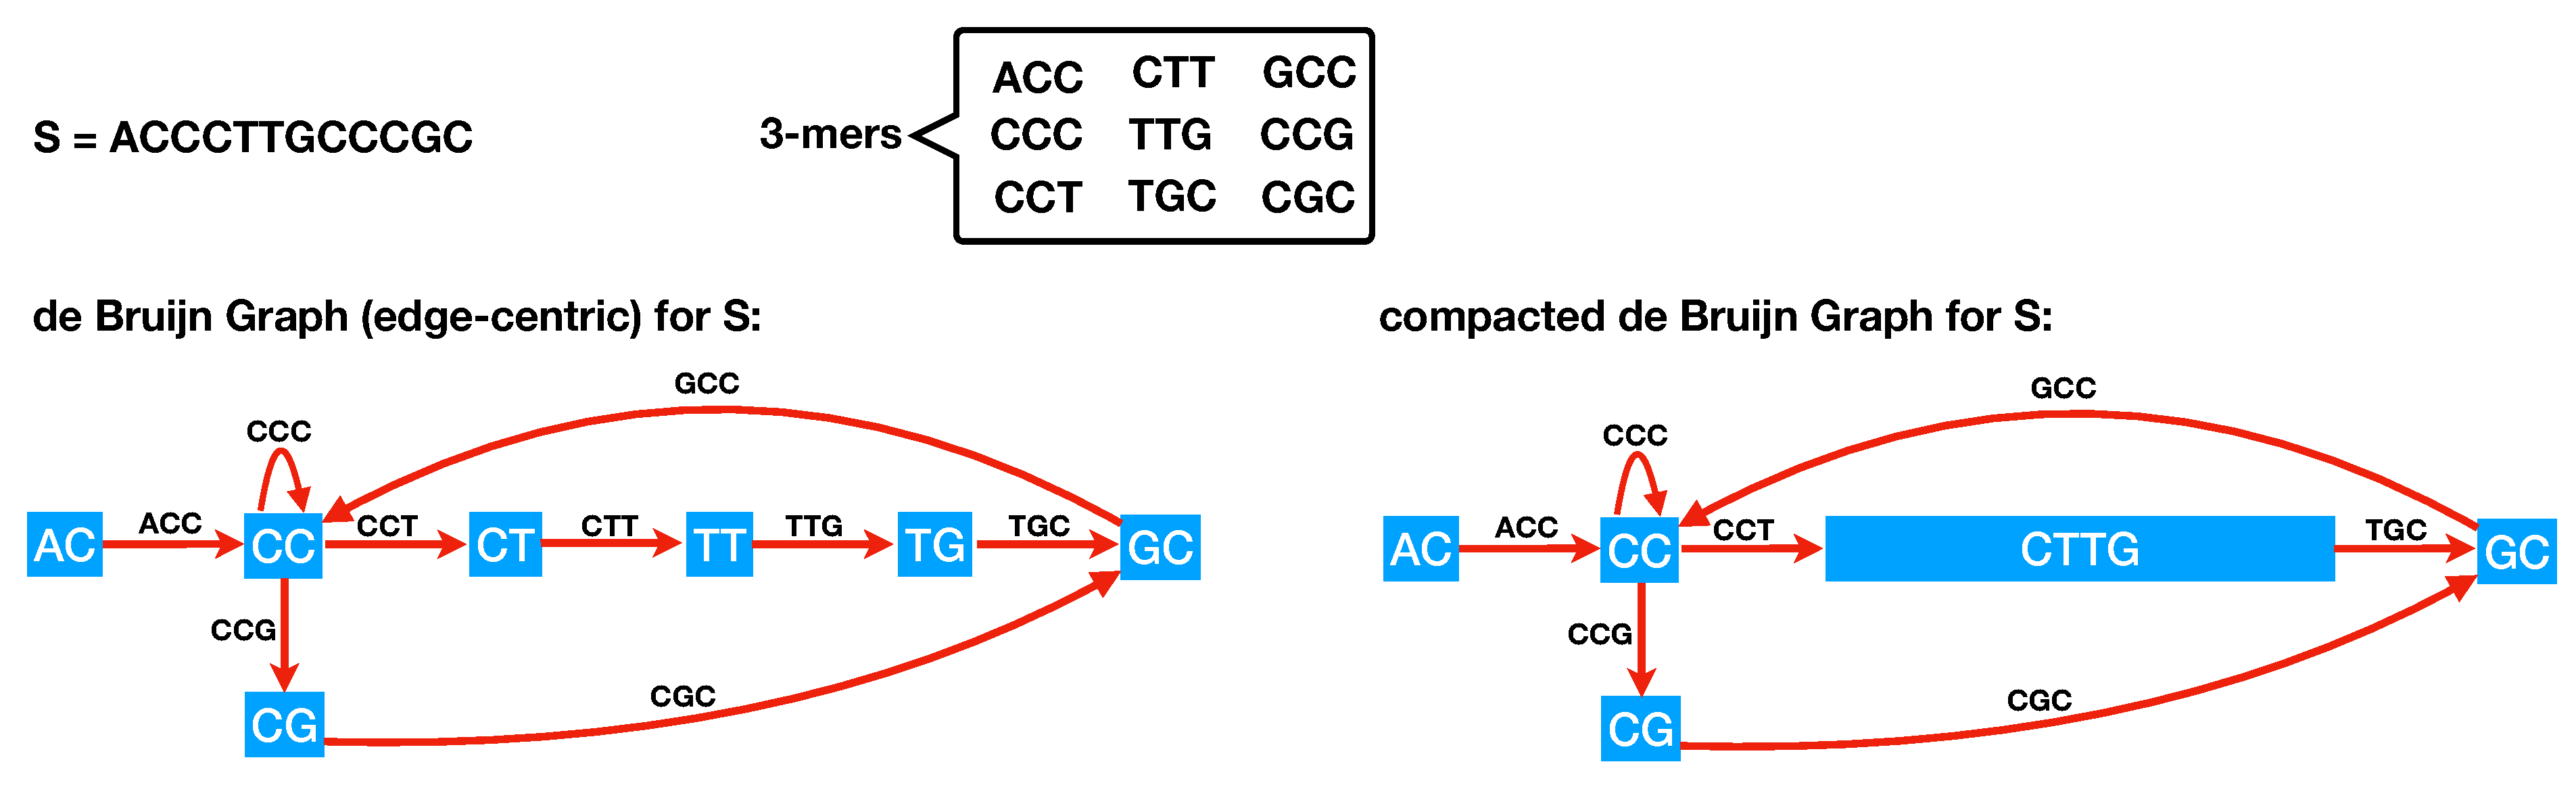
\includegraphics[width=0.95\columnwidth]{Figures/intro/deBruijnGraph.pdf}
 \caption[The edge-centric \dbg]{The edge-centric \dbg and the \cdbg for the 
 sequence S. There are 9 3-mers in this sequence which correspond to the edges 
 in the \dbg. 2-mers form the nodes of the \dbg. 3 nodes (CT, TT and TG) are 
 combined together in the \cdbg since they are on a non-branching path of the 
 \dbg.}
  \label{fig:dbg}
\end{figure}

Another approach for indexing all the \kmers of a set reference sequence is to 
build the \dbg. Each \kmer forms an edge in the \dbg between the 
prefix and suffix k-1 mers that it consists of.~\Cref{fig:dbg} shows a \dbg 
built from the sequence $S = ACCCTTGCCCGC$ and the $k$ 
equal to 3. One main property in the \dbg is that every \kmer 
appears exactly once in the graph. This property helps to reduce the redundancy 
of repeats that usually exist in the DNA and RNA sequences. The \cdbg
is built after compacting the non-branching paths from the 
original \dbg, as shown in the~\cref{fig:dbg}. The length of the 
nodes in the \cdbg might be larger than k-1, but still 
each \kmer appears at most once in the graph (either as an edge or as a 
substring in one node). If the \dbg is built from multiple 
sequences (e.g., the set of human transcripts, or a collection of microbial 
genomes), one is interested to know in which reference sequences each \kmer 
appears. A \kmer might appear in multiple reference sequences due to shared 
exons in transcripts or sequence similarities in different strains of some 
species.

A colored \dbg stores this data for each \kmer (edge) of the graph as the color 
information. For example, in the case of the transcriptome, each color represents 
the set of transcripts in which the \kmer corresponding to that edge exists. 
\Kmers appearing in the same set of transcripts (e.g., due to shared exons) 
will have the same colors. A \unitig in the \cdbg is a non-branching path in 
the graph, and if the edges are colored, not all the \kmers in a \unitig might 
have the same color.
If all the \kmers that are part of a non-branching path also have the same color 
set assigned, those \kmers can be combined together and form a \unitig in the 
\ccdbg.

\pufferfish~\citep{pufferfish} is a space and time efficient index built on 
top of the \ccdbg. So, it can be used to perform 
efficient \kmer queries from each read sequence to large transcriptomic or 
genomic references. 
% In the second chapter of this manuscript, we introduce 
% \puffaligner which uses the \pufferfish index to query \kmers from the short 
% reads to compute read alignments through the seed and extend strategy.
We used \pufferfish index to develop \puffaligner.
\puffaligner queries the \kmers from the read into the \pufferfish
index, which contain all the reference sequences, to find the seeds for alignment.

\subsection{Alignment Free Approaches for Mappings reads}\label{int:qm}
Exploiting the methods of abundance estimation for RNA-seq reads revealed the 
fact that although alignment is very useful for finding the candidate transcripts 
to which reads map, the full alignment information (i.e., exact details of all the 
gaps and mismatches) are unnecessary for performing quantification. In fact the 
position, orientation and length of the matching fragment on each transcript is 
adequate for achieving accurate estimates. Therefore, lightweight methods were 
developed to avoid performing full alignments upstream of the quantification. 
These methods typically build an index over the reference sequence (similar to 
the FM index in alignment tools). Then, in the quantification step, the reads 
are mapped to the reference on the fly using the built-in index. 
Therefore, the peak memory footprint of such methods is bounded by the reference 
size and complexity and scales well with respect to the number of reads increases. Note that 
for performing quantification over multiple samples to the same reference, the 
index needs to be built only once.

The first lightweight algorithm for mapping reads to reference transcripts was 
introduced in \sailfish~\citep{Patro2014Sailfish}. \sailfish is an alignment-free 
quantification tool that builds an index over all subsequences of size $k$ from the 
reference, called \kmers. The \sailfish index consists of a perfect hash function 
mapping each \kmer in the reference to a unique integer, an array indicating the 
counts of each \kmer, an index mapping each \kmer to the set of transcripts 
in which it appears, and another index mapping each transcript to the multiset 
of \kmers it contains. In the quantification step, \sailfish explores all the 
\kmers the read contains and keeps the count for the ones appearing in the 
reference. So instead of mapping the whole reads, \sailfish only maps the \kmers, 
and uses their count for each transcript as evidence for the relative expression 
of the transcripts. Although approach of \sailfish is 30 times faster than fastest 
quantification tools that perform alignment upstream of quantification, 
it suffers from increased ambiguity of a large rate of multi-mapping \kmers, 
which sometimes reduces the accuracy of abundance estimation. The smaller $k$ size 
causes a higher multi-mapping rate, while the larger size of the $k$ results in 
less robustness to sequencing errors because each \kmer is mapped with no error 
using the perfect hash function.

The idea of mapping \kmers instead of the whole reads to reference transcriptome 
introduces a huge improvement in the speed of quantification tools. However, 
it is sub-optimal to only consider occurrence of subsequences of size $k$ as 
evidence of expression while the observed data is of larger length. Hence, 
the developers of \sailfish introduced a new idea for mapping the whole reads 
using the perfect hash function of \kmers by benefiting from the suffix array 
data structure. The new mapping approach is called \Qm~\citep{Srivastava2016rapmap} 
and is utilized in the newer version of \sailfish software and also in the new 
quantification tool called \salmon~\citep{Patro2017Salmon}. 

The suffix array of a sequence is a sorted array of all of the suffixes of the sequence. 
Therefore, all suffixes starting with the same prefix are located in adjacent 
positions of the suffix array. Note that only the position of the occurrence of 
suffixes in $T$ are stored in the suffix array. The number of elements of the 
array is equal to the length of the sequence and there is a one-to-one mapping 
from each row of the suffix array to a character in the BWT of the sequence. We 
can also introduce suffix array intervals similar to intervals of the 
Burrows-Wheeler transform. In the \qm index the suffix array $SA(T)$ is built from 
reference transcriptome $T$. Therefore, each row in the $SA$ starts at a unique 
transcript of the transcriptome. There is a hash function $I(k_i)=[b,c)$ from 
each \kmer $k_i$ in $T$ to a suffix array interval from row $b$ until row $c$; 
all rows that contain $k_i$ as a prefix. For mapping each read, the \kmers, $k_i$ 
of the read (existing in the hash table) are hashed to find SA intervals. It is 
often possible to extend a match between the query and a subset of rows of the SA 
interval. The \qm algorithm attempts to find the longest subsequence of the query 
starting with the $k_i$ as a prefix in the interval (also called maximum mappable 
prefix of $k_i$ ($MMP_i$)~\citep{Dobin2013Star}) with a binary search, as the SA 
is sorted lexicographically.~\citep{Srivastava2016rapmap}
\Qm retrieves a set of transcripts for each \kmer, the transcripts appearing 
in all sets are reported as mapping candidates for the read. The reverse 
complement of the read is also mapped and the sequence (either forward or 
reverse complement) with the higher number of matching \kmers determines the 
mapping orientation. For paired end reads, the other end of the read is also 
quasi-mapped to the reference. Then, transcripts appearing as candidates for 
both ends of the reads are reported as the mapping possibilities for the paired 
end reads.

It has been demonstrated that \qm finds very high quality mappings which result 
in highly-accurate abundance estimations. However, there are different aspects of 
the algorithm that can be modified in order to retrieve mappings with higher 
specificity and sensitivity. In fact, this idea is presented in chapter 2 as 
\sla. \Qm extends the \kmer matches by the MMP length in order to find legitimate 
matches for queries. However, if an extension is not possible and no other \kmer 
match exists in the read, \qm may report all transcripts of the interval as the 
mapping candidates for the read. These low quality matches introduce a number 
of spurious mappings. A new filtering process was introduced in order to further filter 
the spurious hits in this case. Other than suffering from spurious mappings \qm 
could also miss true mappings of the read in rare cases where errors are 
positioned adversarially on the read. An obvious case of losing the true mapping 
is if a read contains no subsequence of size $k$ from the true transcript. In 
another case, the true mapping of the read might be lost from the SA interval 
by performing MMP extension, if a longer exact match of the read to the interval 
masks the match to the row with true location. The hits in the reverse complement 
of the read are only considered if there are less number of hits in forward strand 
compared to reverse complement. Therefore, spurious mappings in the forward strand 
might mask the true hit in the reverse complement. For some reads, multiple 
positions might be found on the same transcript where the read maps. \Qm 
greedily considers the left most one as the true mapping while that might 
not be the best possible matching of the read to that transcript. To address 
these challenges in \qm, \sla is introduced as a new lightweight approach to 
achieve both higher sensitivity and specificity than \qm.

A similar approach to \qm is employed in \kallisto~\citep{Bray2016Kallisto} 
called \pa. \Kallisto index consists of a colored \dbg from reference 
where nodes are \kmers and each node receives the colors of transcripts in which 
it appears. The \unitigs in the graph are formed from the linear stretches of the 
nodes (\kmers) with identical sets of colors. \Kallisto also maintains a hash 
table mapping each \kmer to the \unitig it is contained in and the position of the \kmer 
in the \unitig. Using this index, the reads' \kmers are mapped to \unitigs. Since 
all the \kmers appearing in the same \unitig receive the same set of colors, and 
therefore the same transcripts, the rest of the \kmers in the \unitig can be 
skipped for mapping, similar to the idea of skipping to 
the next informative position (NIP) in \qm.

\section{Abundance estimation of the transcriptome}
In this section, we formalize the problem of abundance estimation with RNA-seq 
reads according to the model laid out by \rsem~\citep{Li2010RSEM}. There are $M$ 
transcript types in transcriptome $T$, $t_1, t_2, ..., t_M$. In a given sample 
there are $c_i$ copies of transcript type $t_{i}$, which are not observed directly.
Existence of more copies of a transcript indicates its higher expression in the sample
compared to other transcripts, which is generally proportional to the number of 
proteins generated from that transcript. Therefore, quantification of transcriptome
is used as an indicator for the expression level of proteins as well.

\subsection{The generative model of a sequencing experiment}
%\label{subsec:likelihood}

The generative model of RNA-seq experiments states that the number of fragments 
sequenced from $i^{th}$ transcript type is proportional to the total number of 
sequenceable nucleotides belonging to transcripts of type $t_i$. If the length 
of the $i^{th}$ transcript is given by $l_i$, assuming all the reads have the 
size $l_r$, we can define effective length, $\tilde{l}_i = l_i-l_r+1$ which is 
all possible start positions on transcript $t_i$ for sequencing a read of size 
$l_r$. The portion of sequenceable nucleotides of transcript type $t_i$ is 
$ \eta_i = \frac{c_il_i}{\sum_{j}{c_jl_j}}$ and $\alpha_i \propto \eta_i$, 
where $\alpha_i$ is the number of fragments drawn from transcripts of type $t_i$.

If $\fragments$ with $|\fragments|=N$, is the set of sequenced fragments, 
assuming independence for drawing each fragment, the likelihood of the underlying 
transcript abundances, $\theta$, can be written as:

\begin{equation}
  \likelihood{\bm{\theta}; \fragments} = \prod_{f_j \in \fragments}  
  \sum_{j=1}^{M} \Pr\left(t_i \mid \bm{\theta}\right) 
  \Pr\left( f_j \mid t_i \right).
  \label{eqn:likelihood_fm1}
\end{equation}

The conditional probability of drawing a particular fragment $f_j$, given 
transcript $t_i$, $\Pr{(f_j|t_i)}$, is particularly critical for reaching 
accurate estimates and is derived from mapping information.  This term encodes, 
given parameters of the model and experiment, how likely it is to observe a 
specific fragment $f_j$ arise from transcript $t_i$.
Many terms can be included in such a conditional probability, 
some common terms include:

\begin{equation}
  \Pr\left( \fraglen{j} \mid f_j, t_i\right) = \frac{\Pr_D\left( \fraglen{j}\right)}{\sum_{k=1}^{\tilde{l}_i} \Pr_D\left( k \right)},
  \label{eqn:pr_len1}
\end{equation}

the probability of observing a mapping of implied length $\fraglen{i}$ 
for $\frag{i}$ given that it derives from $\txp{j}$, where $\Pr_D\left(k\right)$ 
is the probability of observing a fragment of length $k$ under the empirical 
fragment length distribution $D$;

\begin{equation}
  \Pr\left( p_j \mid \fraglen{i}, f_j, t_i\right) = \frac{1}{l_i - \fraglen{j} + 1},
  \label{eqn:pr_start1}
\end{equation}

the probability of a observing a mapping starting at position $p_i$ for 
fragment $\frag{i}$ given that it has implied length $\fraglen{i}$ and is 
derived from $\txp{j}$;

\begin{equation}
  \Pr\left( o_i \mid \frag{i}, \txp{j} \right)  = 
  \begin{cases}
    \begin{cases}
      0.5 
    \end{cases}
    & \text{if the library is unstranded}\\
    \begin{cases}
      1.0 - \epsilon & \text{if compatible orientation} \\
      \epsilon & \text{if incompatible orientation}
    \end{cases} &\text{if the library is strand-specific}
  \end{cases},
  \label{eqn:orient1}
\end{equation}

the probability of observing a mapping with a specific orientation $o_j$ 
(i.e., forward or antisense) with respect to the underlying transcript for 
$\frag{j}$, given $\txp{i}$, $\epsilon$ (a user-defined constant), and knowledge 
of the underlying protocol, 
and

\begin{equation}
   \Prob{a_i}{\frag{i}, o_i, \fraglen{i}, p_i, \txp{j}},
  \label{eqn:align1}
\end{equation}

the probability of observing the particular alignment (e.g., \texttt{CIGAR}
string) $a_i$ for $\frag{i}$ given it is sampled from transcript $\txp{j}$, has
orientation $o_i$, implied length $\fraglen{i}$ and starts at position
$p_i$---such a probability is calculated from a model of alignments, like those 
presented in~\citep{Li2010RSEM,Roberts2013Express,Patro2017Salmon}.

In fact, one can conceive of many such general models of ``fragment-transcript
agreement''~\citep{Patro2017Salmon}. However, here we consider that 
$\Prob{f_j}{t_i}$ is simply the product of the conditional probabilities 
defined in~\Cref{eqn:pr_len1,eqn:pr_start1,eqn:orient1,eqn:align1}, appropriately 
normalized.


\subsection{Expectation-Maximization for optimizing the model parameters}
Exact inference from the likelihood function is intractable for the large 
scale of RNA-seq data. Local optimization methods, like expectation 
maximization (EM), are often applied to fit the best parameters in the model. 
The parameters of the model indicate the rate of expression for each transcript 
in the underlying samples. The EM approach is employed by both alignment based 
tools such as \rsem~\citep{Li2010RSEM}, \mmseq~\citep{Turro2011Haplotype}, and
\isoem~\citep{Nicolae2011Estimation}, and also non-alignment based tools, e.g., 
\sailfish~\citep{Patro2014Sailfish}, \salmon~\citep{Patro2017Salmon}, and 
\kallisto~\citep{Bray2016Kallisto}. 

\begin{algorithm}[H]
\SetAlgoLined
\KwData{$T = \{t_i\}$,
        $\fragments = \{f_j\}$,
        $\Pr{(f_j|t_i)}$ for all fragment transcript pairs, \\
        $\elength{i} = \length{i}-\mu$,
        where $\mu$ is the mean of the empirical fragment length distribution
        and $\length{i}$ is the length of the transcript $t_i$.}
\KwResult{$\theta$, relative abundance of transcripts}
\textcolor{blue}{Uniform initialization:}\\
\For{$t_i \in T$}{
  $\alpha_i \leftarrow 0$, $\theta_i \leftarrow \frac{1}{|T|}$ 
}
\While{not converged}{
  \textcolor{blue}{E-step:} \\
  \For{$f_j \in \fragments$}{
  $sum \leftarrow \sum_{t_k \in T}{\theta_k \times  \Pr{(f_j|t_k)}}$\\
    \For{$t_i \in T$}{
      $\alpha_i \leftarrow \alpha_i + \frac{\theta_i \times  \Pr{(f_j|t_i)}}{sum}$
    }
  }
  \textcolor{blue}{M-step:} \\
  $sum \leftarrow \sum_{t_k \in T}{\frac{\alpha_k}{\tilde{l_k}}}$\\
  \For{$t_i \in T$}{
    $ \theta_i \leftarrow \frac{\alpha_i/\tilde{l_i}}{sum}$, $\alpha_i \leftarrow 0$
  } 
}
\caption{Overview of the EM algorithm for optimizing the generative model}
 \label{EM-alg}
\end{algorithm}

The overview of the EM algorithm for optimizing~\cref{eqn:likelihood_fm1} is 
displayed in algorithm \ref{EM-alg}. In the E-step, the expected number of 
fragments sequenced from each transcript type in the sample is calculated. 
Using these expectations, alongside effective lengths the prior probability of 
observing each transcript type is obtained in the M-step. This iterative process 
is repeated until the convergence on $\theta$ values is reached. 

If a transcript $t_i$ is not present in the set of transcripts to which 
fragment $f_j$ is mapped, the  value of $\Pr{(f_j|t_i)}$ is equal to zero. 
The EM updates can benefit from the sparsity of $\Pr{(f_j|t_i)}$ matrix by 
only performing updates in the E-step for the set of transcripts that $f_j$ maps 
to instead of the whole set of transcripts. Hence, if $\Omega{(f_j)}$ is the set 
of compatible transcripts with read $f_j$, in algorithm~\ref{EM-alg}, the line 8 
shall be modified to : 
$sum = \sum_{t_k \in \Omega{(f_j)}}{\theta_k \times  \Pr{(f_j|t_k)}}$\  
and the loop iteration in line 9 to :   $t_i \in \Omega{(f_j)}$.

\subsection{Factorizations of the likelihood function}\label{int:fact}

Each iteration of the EM algorithm updates the $\alpha$ values for each fragment 
independently. Although each update cost has collapsed considerably by benefiting 
from the sparsity of mapping matrix, the number of EM updates still scales with 
the number of fragments (and alignments). Sequence similarities in reads are 
utilized for factorizing the likelihood function, which results in bounding the 
number of updates as the number of fragments grows.
 
If a set $F'$ of fragments exactly map to the same set $T'$ of transcripts 
with the same conditional probabilities (meaning that for each pair 
$f_a,f_b \in F'$, $\Omega{(f_a)}=\Omega{(f_b)}=T'$ and the equation 
$\Pr{(f_a|t_k)}=\Pr{(f_b|t_k)}$ holds for all $t_k \in T'$), then all 
fragments in $F'$ are exactly equivalent, and they result in the same update rule 
in the EM iterations. Hence, they can be grouped together to apply the update once 
for all such fragments. The factorization introduced by 
\isoem~\citep{isoem}, maintains full fidelity to information regarding fragment 
mappings to transcripts because all fragments in a group are identical.

A more popular approach for factorizing the likelihood is employed by 
\mmseq~\citep{Turro2011Haplotype} and also later in alignment-free tools 
like \sailfish~\citep{Patro2014Sailfish}, \salmon~\citep{Patro2017Salmon} 
and \kallisto~\citep{Bray2016Kallisto}. \Mmseq introduced a notion of fragment 
equivalence classes, which treats as equivalent any fragments that map to the 
same set of transcripts. Unlike \isoem, the equivalence notion does not depend 
on the values of conditional probabilities.  According to this definition, every 
set of fragments like $\Frags^q$ such that for all 
$f_a,f_b \in \Frags^q$, $\Omega{(f_a)}=\Omega{(f_b)}=\Omega{(\Frags^q)}$, 
form an equivalence class with the label $\Omega{(\Frags^q)}$. 
Define $N^q=|\Frags^q|$ to be the number of fragments in class $\Frags^q$. 
Then, the likelihood function based on these equivalence classes, can be 
approximated as:

\begin{equation}
    \likelihood{\bm{\theta}; \Frags} \approx 
        \prod_{\eqclass{q} \in \eqclasses}
        \left(\sum_{\langle i, t_i \rangle \in \mapset{\eqclass{q}}} 
        \Prob{\txp{i}}{\bm{\theta}} 
        \cdot \Prob{f_q}{\eqclass{q},\txp{i}} \right)^{\eqsize{q}},
\label{eqn:likelihood_fact}
\end{equation}

where $\eqclasses$ is the set of all equivalence classes, and
$\Prob{f_q}{\eqclass{q},\txp{i}}$ is the probability of generating a fragment $f_q$
given that it comes from equivalence class $\eqclass{q}$ and transcript
$\txp{i}$. The key to the efficiency of likelihood evaluation (or optimization)
under this factorization, is that the probability $\Prob{f_q}{\eqclass{q},\txp{i}}$ 
is assumed to be identical for each of the $\eqsize{q}$
fragments in each equivalence class $\eqclass{q}$---hence, we do not
subscript $f$ in~\cref{eqn:likelihood_fact}. This allows one to replace the
product over all fragments $f_j$ in full model (\cref{eqn:likelihood_fm1}) with 
a product over all equivalence classes in \cref{eqn:likelihood_fact}. 
The approximation, of course, stems from the fact that, under the full model, 
a fragment $\frag{j}$ may have a probability 
$\Prob{\frag{j}}{\txp{i}}$ that is arbitrarily different
from $\Prob{f_q}{\eqclass{q},\txp{i}}$, where $f_q$ represents
all the fragments in equivalence class $\eqclass{q}$ which are assumed to be identical.
 Moreover, the most common approximations,
like those adopted in \mmseq, \sailfish, and \kallisto consider this
probability to be fixed and essentially independent of any fragment-level
information (e.g., it is set to one divided by the effective
length of $\txp{i}$).

After applying any factorization to group a set of fragments together 
in equivalence classes $\Frags^q$, the fragments in the EM iteration can 
be substituted with equivalence classes (groups) and each update would 
increase the $\alpha$ values based on the number of fragments in each 
equivalence class. The modified version of the E step 
in algorithm \ref{EM-alg} is displayed in algorithm \ref{EM-alg2}.

\begin{algorithm}[H]
\textcolor{blue}{E-step:} \\
\For{$\Frags^q \in \eqclasses$}{
 $sum = \sum_{t_k \in \Omega{(\Frags^q)}}{\theta_k \times  \Pr{(f|\Frags^q,t_k)}}$
 \\
 \For{$t_i \in \Omega{(\Frags^q)}$}{
    $\alpha_j += \frac{\theta_k \times  \Pr{(f|\Frags^q,t_k)}}{sum}$
 }
}
\caption{Modified E step after employing factorization}
 \label{EM-alg2}
\end{algorithm}


\subsection{Online EM for optimizing the likelihood function}

The conditional probability values are stored in memory during the EM iterations 
in order to avoid expensive I/O operations and re-computation in each EM round. 
If no factorization is used, for each existing mapping pair $f_j$ and $t_i$, 
a value is stored. This makes the memory requirement scale with the number of 
mappings. \express~\citep{Roberts2013Express} attempts to bound the memory 
requirement by benefiting from an online-EM algorithm rather than a batch-EM. 
An online-EM consists of a single iteration over all fragments in the sample, 
updating $\alpha$ values once for each fragment. Fragments are not stored in 
memory after being observed, which makes memory require of \express 
independent of the number of fragments in the sample. The large number of 
fragments in RNA-seq samples lets \express often achieve high quality abundance 
estimates with a single run over the data. \express requires the output 
of an alignment tool for mapping reads to transcripts to run the online phase. 
Again, here the mapping information shall limit the number of updates performed 
for each fragment. 

\express applies a modified version of online updates to prevent the 
algorithm from performing updates for each transcript in each iteration. 
The online update rules for each fragments are:
\begin{equation}
\alpha^{i+1} = \alpha^{i}+m_i\tilde{\tau}^i,
\label{eqn:online1}
\end{equation}
where:
\begin{equation}
\tilde{\tau}^i_t =\Pr{(T=t|F=f_j)},
\label{eqn:online2}
\end{equation}
and
\begin{equation}
m_{i+1} = m_i \times \frac{\gamma_{i+1}}{1-\gamma_i} \times \frac{1}{\gamma_i},
\label{eqn:online3}
\end{equation}

$\alpha^i$ is the optimized value after observing the first i fragments. 
Bayes' rule can be applied to obtain the probability in \cref{eqn:online2} 
from the conditional probabilities. The value $m_i$ is called forgetting 
mass and depends on the forgetting factor $\gamma_i$. The $\gamma$ values 
are set as $\gamma_i=\frac{1}{i^c}$ where $0.5<c<1.0$. After observing 
all $N$, fragments the relative counts of fragments from each transcript type 
can be obtained from the vector $\alpha^N$.

\subsection{Dual phase optimization}
The inference algorithm in \salmon~\citep{Patro2017Salmon} consists of two phases. 
First, \salmon runs an online EM optimization to obtain high quality primary 
estimates of abundances. In this phase, \salmon is able to achieve a good 
estimation of fragment length distribution by examining many fragments as 
they are streamed in the online EM. Therefore \salmon can derive good estimates 
of conditional probabilities using the fragment length distribution and other 
information provided with mappings. The equivalence classes over sets of 
fragments are also created in the online phase. \salmon introduces the notion 
of rich equivalence classes by assigning a single scalar to each transcript in 
an equivalence class, averaging the conditional probabilities of all fragments 
in the class to the transcript. This value is equal to $\frac{1}{|\Omega{(F^q)}|}$ 
in non-rich equivalence classes. 

\salmon uses the estimates obtained in the online phase as a starting point 
for performing a batch EM algorithm in the second phase. This two-phase 
optimization allows \salmon to rich very high quality estimates compared 
to other existing quantification tools. The online phase of the \salmon 
enables deriving a new factorization of the likelihood function to be 
optimized in the batch EM phase, which does not discard any necessary 
information for accurate abundance estimation. The details of this 
factorization is discussed in chapter 3.

\subsection{Metrics for evaluating quantification accuracy}
The formula for calculating the metrics used for evaluating the 
abundance estimation results in the manuscript are as follows. 
The metrics are Mean Absolute Relative Difference (MARD), Mean Absolute
Error (MAE), and Mean Squared Error (MSLE).

\begin{equation}
\begin{split}
    \text{MARD}(y, \hat{y}) = \frac{1}{n_{\text{refs}}} 
    \sum_{i=0}^{n_{\text{refs}}-1}
    {\frac{ \left| y_i - \hat{y}_i \right|}{y_i + \hat{y}_i}}. 
    \\
    \text{MAE}(y, \hat{y}) = \frac{1}{n_{\text{refs}}} 
    \sum_{i=0}^{n_{\text{refs}}-1} \left| y_i - \hat{y}_i \right|. 
    \\
    \text{MSE}(y, \hat{y}) = \frac{1}{n_\text{refs}} 
    \sum_{i=0}^{n_\text{refs} - 1} (y_i - \hat{y}_i)^2. 
    \\
\end{split}
\label{eq:metrics}
\vspace{-7mm}
\end{equation}

All of these metrics compute the difference of the estimated abundances 
with the truth. In addition to these metrics, we also evaluate the 
correlation between the estimations and truth by computing the 
Spearman correlation. Spearman correlation is computed using the 
pandas library~\citep{reback2020pandas} in Python.

\subsection{Inference of the Posterior Distribution of RNA-seq quantification}
Estimating the inference uncertainty of the RNA-seq quantification is one of the crucial
steps for many downstream analysis, e.g., finding the differentially expressed genes or 
transcripts, i.e., DE analysis. In fact, methods like Swish~\citep{zhu2019nonparametric}
directly use the inferential replicates created by RNA-seq quantification tools for finding
the DE genes with a higher precision compared to other approaches.

There are two main approaches for sampling the posterior distribution for estimating the 
uncertainty of quantification estimates; \gibbs and \boots. 
The \gibbs is a Markov chain Monte Carlo (MCMC) procedure
that walks through the space that the EM explores for finding the \mles of the transcripts expressions.
At the end of each iteration of the \gibbs, the transcript expression vector could be identified
as a new inferential replicate for estimating the posterior distribution. To decrease between
replicate correlations, the sampling could take place after every fixed number of iterations which
is called the thinning factor for the sampling. Running the \gibbs procedure for long enough 
could reach to the convergance of the posterior estimate, this will be reached only after
the Gibbs sampler has explored all the posterior samples. The number of iterations
required for \gibbs to converge depends on the properties of the sample, and as the number
of transcripts in the sample increases the convergance usually takes longer.

% talk about bootstrap sampling
\boots is the other main approach for estimating the posterior distribution of the abundance
estimations in RNA-seq. The bootstrap procedure~\citep{efron1979computers} is a widely-used 
and computationally straightforward procedure for calculating measures of accuracy of an 
estimator. It works by resampling (with replacement) from the observed data, and treating 
these as population samples. The procedure has been used in many contexts for non-parametric 
estimation. In RNA-seq, computing the abundance estimation of all \boot replicates leads to a 
estimating a posterior distribution for the abundances. 

% talk about the current methods available for estimating the posterior
RNA-seq quantification tools~\citep{kallisto,salmon} have implemented the regular bootstrap 
sampling by resampling the \eqc counts. \Eqcs are a summerized representations of the reads; 
therefore, sampling the \eqc counts instead of each individual read improves the efficiency 
of the \boots. \Pboots is also another way of generating \boot replicates by sampling the 
positions where the reads map to on each transcript~\citep{xiong2016probabilistic}.
Furthermore, the RNA-seq quantification tool, \salmon~\citep{salmon} also includes a \gibbs
procedure for estimating the posterior distribution. \bitseq~\citep{glaus2012identifying} 
applies a MCMC \gib sampler to generate samples from the posterior probabilty distribution. 

\section{Overview of the document and contribution}
In the first chapter, I discussed about some of the main important computational steps
for analysis of RNA-seq data including alignment and quantification.
In chapter 2, novel methods are presented for improving the accuracy and efficiency of 
short read mapping. More specifically, I have contributed in development 
of \sla~\citep{selaln} which improves
the accuracy of lightweight mapping without a significant effect on their efficiency.
Furthermore,  \puffaligner~\citep{almodaresi2021puffaligner} 
will be discussed in chapter 2 which is an accurate aligner for short reads
to a set of references which maintains a moderate memory usage while being very fast.
In chapter 3, I present an improved factorization of the RNA-seq likelihood~\citep{ddfact} 
which bridges the accuracy gap between the approximate and full models and has almost 
no effect on the efficiency of fast RNA-seq quantification approaches.
In chapter 4, I attempt to improve the uncertainty estimation of RNA-seq quantification by 
introdcing the augmented Bootstrap. More particularly, I will discuss how this approach 
improves estimating the posterior distrubtion of abudance estimation of allelic expressions.

% \textbf{Contributions:}
% \begin{description}
%   \item[$\bullet$~\cref{chapt2}] I present two main papers. The first one is \sla~\citep{selaln} which
%   is a joint work with Hirak Sarkar. We both contributed equally in design, coding and writing. 
%   In the second part of the chapter, I prsent \puffaligner~\citep{almodaresi2021puffaligner} which
%   is a joint work with Fatemeh Almodaresi. We both contirbuted equally in coding, design and writing.
%   \item[$\bullet$~\cref{chapt3}] I present
%   \item[$\bullet$~\cref{chapt4}] 
% \end{description}
%%Chapter 2

\renewcommand{\thechapter}{2}

\chapter[Alignment and mapping metods]
{Improving accuracy and speed of mapping and alignment methods}
\label{chapt2}

In this chapter, I explore new ideas for improving the alignment and mapping methods. 
In the first part of the chapter, I address some of the existing obstacles with the 
lightweight  alignment approaches. These methods are employed in the recent non-alignment 
based quantfication tools such as salmon~\citep{Patro2017Salmon}, and 
kallito~\citep{Bray2016Kallisto} to map the RNA-seq reads to the set of known reference 
sequences instead of aligning the reads. We show that the accuracy of the lightweight 
quantification methods decline in the difficult cases which often exist in the real 
samples. We introduce a new algorithm for selectively aligning RNA-seq reads to a 
transcriptome, with the goal of improving transcript-level quantification in adversarial 
scenarios.
\footnote{This is a joint project with Hirak Sarkar and is presented in BCB 2017~\citep{selaln}}

Furthermore, in the second section of this chapter, we build upon the idea of selective 
alignment to introduce Puffaligner~\citep{almodaresi2021puffaligner}, an all purpose 
aligner for short read sequencing reads which can be used in many cases ranging from 
alignment of RNA-seq, DNA-seq and metagenomic samples to known set of references. 
Puffaligner indexes the reference sequences using the Pufferfish index~\citep{pufferfish} 
which efficiently indexes the \cdbg built from the reference sequences.\footnote{This is 
a joint project with Fatemeh Almodaresi and is published in 
Bioinformatics~\citep{almodaresi2021puffaligner}}


\section{Towards Selective Alignment}

While alignment is a staple of many genomic analyses, it sometimes represents more 
information than is actually necessary to address the analysis at hand. For example, 
recent tools like \sailfish~\citep{Patro2014Sailfish}, \rnaskim~\citep{zhang2014rna}, 
\kallisto~\citep{Bray2016Kallisto}, \salmon~\citep{Patro2017Salmon}, and 
\fleximer~\citep{ju2017fleximer}, demonstrate that accurate quantification estimates can 
be obtained without all of the information encoded in traditional alignments. By avoiding 
traditional alignment procedures, these tools are much faster than their alignment-based 
counterparts. Furthermore, by building the mapping phase of the analysis directly into the 
quantification task, they dispense with the need to  write, store, and read, large 
intermediate alignment files. However, these \nab tools, while highly-efficient, have 
the disadvantage of potentially losing sensitivity or specificity in certain cases where 
alignment-based methods would perform well. For example, in the presence of paralogous 
genes, with high sequence similarity, there is an increased probability that the mapping 
strategies employed by such tools, and the efficient heuristics upon which they rely, will 
mis-map reads between the paralogs (or return a more ambiguous set of mapping locations 
than an aligner, which expends computational resources to verify the returned alignments) 
\citep{axtell2014butter}. Similarly, in the case of \textit{de novo} assemblies, poorly 
assembled contigs may have a larger number of mis-mapped reads due to lower sensitivity 
(here, the issue would be primarily due to aberrant exact matches masking the true origin 
of a read).

Other than suffering from spurious mappings, these fast \nab approaches can also miss true 
mappings of a read in rare cases where errors are positioned adversarially on the read. 
An obvious case of losing the true mapping is if a read contains no subsequence of 
sufficient length from the true transcript. In another case, the true mapping of the 
read might be lost from the set of potential mapping loci due to the greedy nature of 
the mapping procedures. For some reads, multiple positions might be found on the same 
transcript where the read maps. In such cases, improved heuristics are required to address 
these challenges. In this section, we present a novel algorithm, \sla, that extends 
quasi-mapping to compute and store edit distance information where necessary. The reads 
for alignment are chosen based on certain criteria calculated during mapping.  This strikes 
a balance between speed and accuracy; not compromising the superior speed of \nab 
algorithms, while also addressing some of the challenges mentioned above. Specifically, 
the motivation for \sla is to enhance both the sensitivity and specificity of fast mapping  
algorithms by reducing or eliminating cases where spurious exact matches mask true mapping 
locations as well as cases where small exact matches support otherwise poor alignments. 
\Sla algorithm is built atop the framework of \rapmap~\citep{Srivastava2016rapmap}, 
which uses an index that combines a fixed-length prefix hash table and an uncompressed 
suffix array~\citep{Manber:1993:Suffix}.  We introduce a coverage-based consensus 
scheme to identify critical read candidates for which alignment is necessary.

Furthermore, we explore the challenging cases where the heuristics employed by fast mapping 
algorithms may fail to locate the correct locations for a read, while the traditional 
aligners do not. We do this by making a number of modifications to the underlying mapping 
algorithm to increase its sensitivity.  We also introduce multiple filters and scoring 
schemes designed to eliminate spurious mappings (i.e., situations where the best mapping 
is unlikely to represent the true origin of the read). In this work, we focus on the effect 
of selective-alignment on transcript quantification estimates, and we leave a thorough 
evaluation of the alignment qualities themselves as future work. In particular, the 
evaluation of alignment qualities is considerably complicated due to prevalent 
multi-mapping in the transcriptome.

\subsection{Main characteristics of \sla}

The process of \sla builds upon the basic data structures of~\citet{Srivastava2016rapmap}, 
but there are a number of important algorithmic distinctions. Specifically, compared to 
the algorithm of RapMap, \sla introduces the k-safe longest common prefix (\kslcp), 
replaces maximum mappable prefixes (MMP) with maximum mappable safe prefixes (MMSP), 
increases mapping sensitivity by adopting a different consensus rule over hits, makes 
use of co-mapping to filter and prioritize potential mapping loci, introduces a new 
mechanism for selecting a mapping position for a read when multiple candidates exist on 
the same transcript, and, finally, introduces a fast edit distance filter (with alignment 
sub-problem caching) to remove spurious mappings and provide quality scores for 
mappings that pass the filter. A block diagram of different steps used in the selective 
alignment pipeline is shown in~\cref{fig:block_overview}.

Below, we recapitulate the basic data structures and concepts that will be required to 
explain the selective alignment algorithm. To start with, the index built on the 
transcriptome in \sla is a combination of a suffix array and a hash table constructed 
from unique \kmers (substrings of length $k$) and suffix array intervals. The suffix 
array of a sequence, $T$--- denoted $SA(T)$---is an array of starting positions of all 
suffixes from $T$ in the original sequence. The values in the array are sorted 
lexicographically by the suffixes they represent. Therefore, all suffixes starting 
with the same prefix are located in adjacent positions of the suffix array. Formally, 
given a suffix array, $SA(T)=\SuffixArray$, constructed from the transcriptome sequence, 
$T$, we construct a hash table, $h$, that maps each \kmer, \samplekmer, to a suffix array 
interval, $\ival{\samplekmer} = \interval{b}{e}$, if and only if all the suffixes within 
interval $\interval{b}{e}$ contain the \kmer \samplekmer as a prefix. We define 
$\SuffixArray[i]$, for every $0\le i \le |\SuffixArray|$, to be the suffix $T[SA[i]]$ 
(i.e., the suffix of $T$ starting from position $SA[i]$). In the \sla index, in addition to 
suffix array intervals, we store two extra pieces of information for each interval; the 
longest common prefix (LCP) and the \kslcp corresponding to the interval. The longest 
common prefix (LCP) of any pair of suffixes in the suffix array is simply the length of 
the prefix that these suffixes share. Though the LCPs for the suffixes in the suffix array 
can be pre-computed, we instead compute them on demand using a linear scan. These methods 
are detailed below. As an alternate to the suffix array and the LCP array, one could make 
use of other data structures which also encode this information. For example, the 
recently-introduced method, Fleximer ~\citep{ju2017fleximer} makes use of the suffix 
tree for selecting informative sig-mers~\citep{zhang2014rna} from the transcriptome, and 
matching reads against them.

\begin{figure}
 \centering
 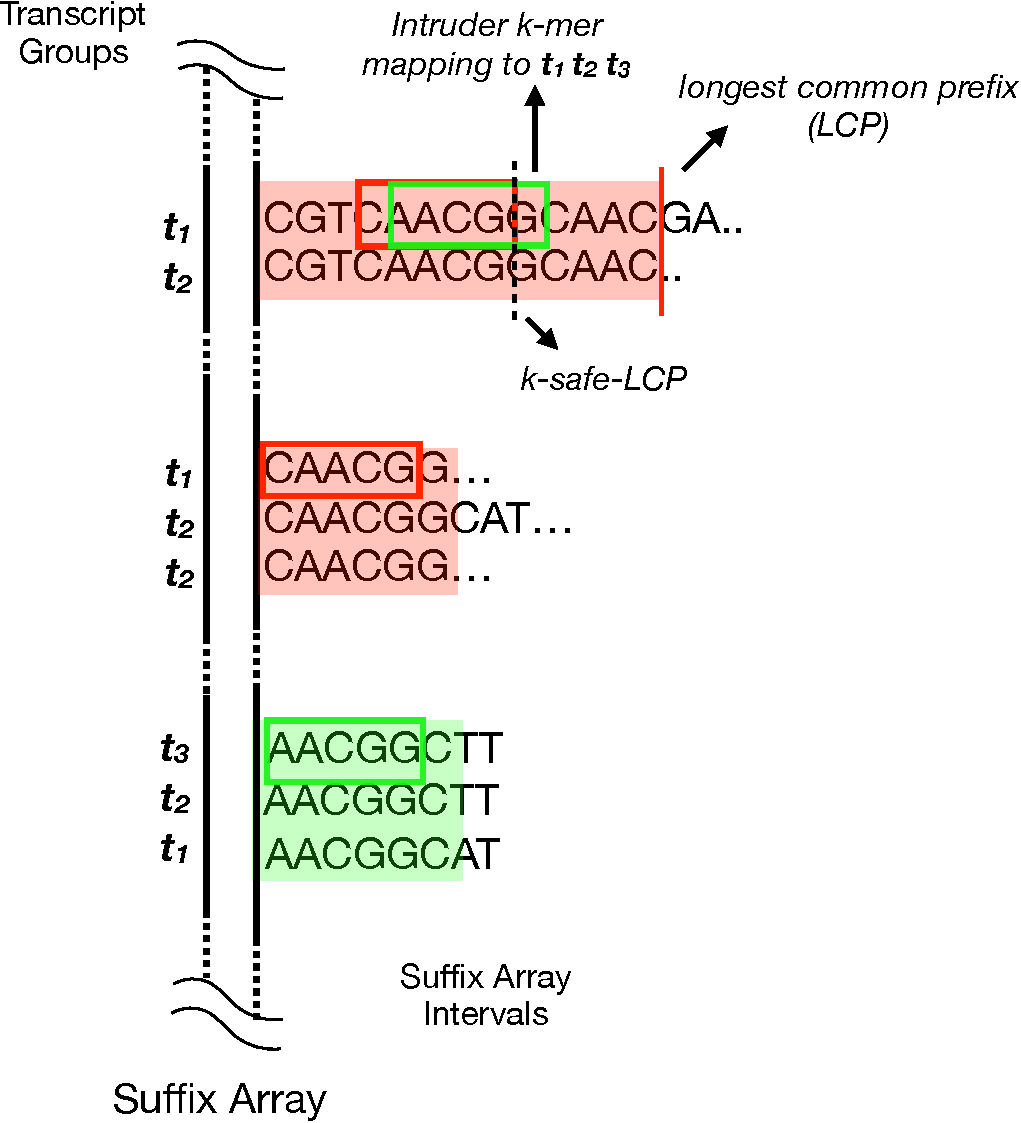
\includegraphics[scale=0.25]{Figures/sla/ksafelcp}
 \caption[Calculation of \kslcp from the suffix array data structure]
    {Calculation of \kslcp from the suffix array data structure. The
    transcripts present in each suffix array interval determine the relevant
    transcript sets, and which \kmers will be considered as intruders. To
    determine the \kslcp of the suffix array interval starting with the \kmer
    $CGTCA$, we check all the \kmers sequentially. Some \kmers do not yield an
    interval with transcripts other than $t_1$ and $t_2$, e.g., $CAACG$.
    Detection of a \kmer ($AACGG$) (as intruder) that maps to suffix array interval 
    labeled $(t_1,t_2,t_3)$ determines the \kslcp here.}
    \label{fig:safelength}
\end{figure}

\begin{figure}%[h]
 \centering
 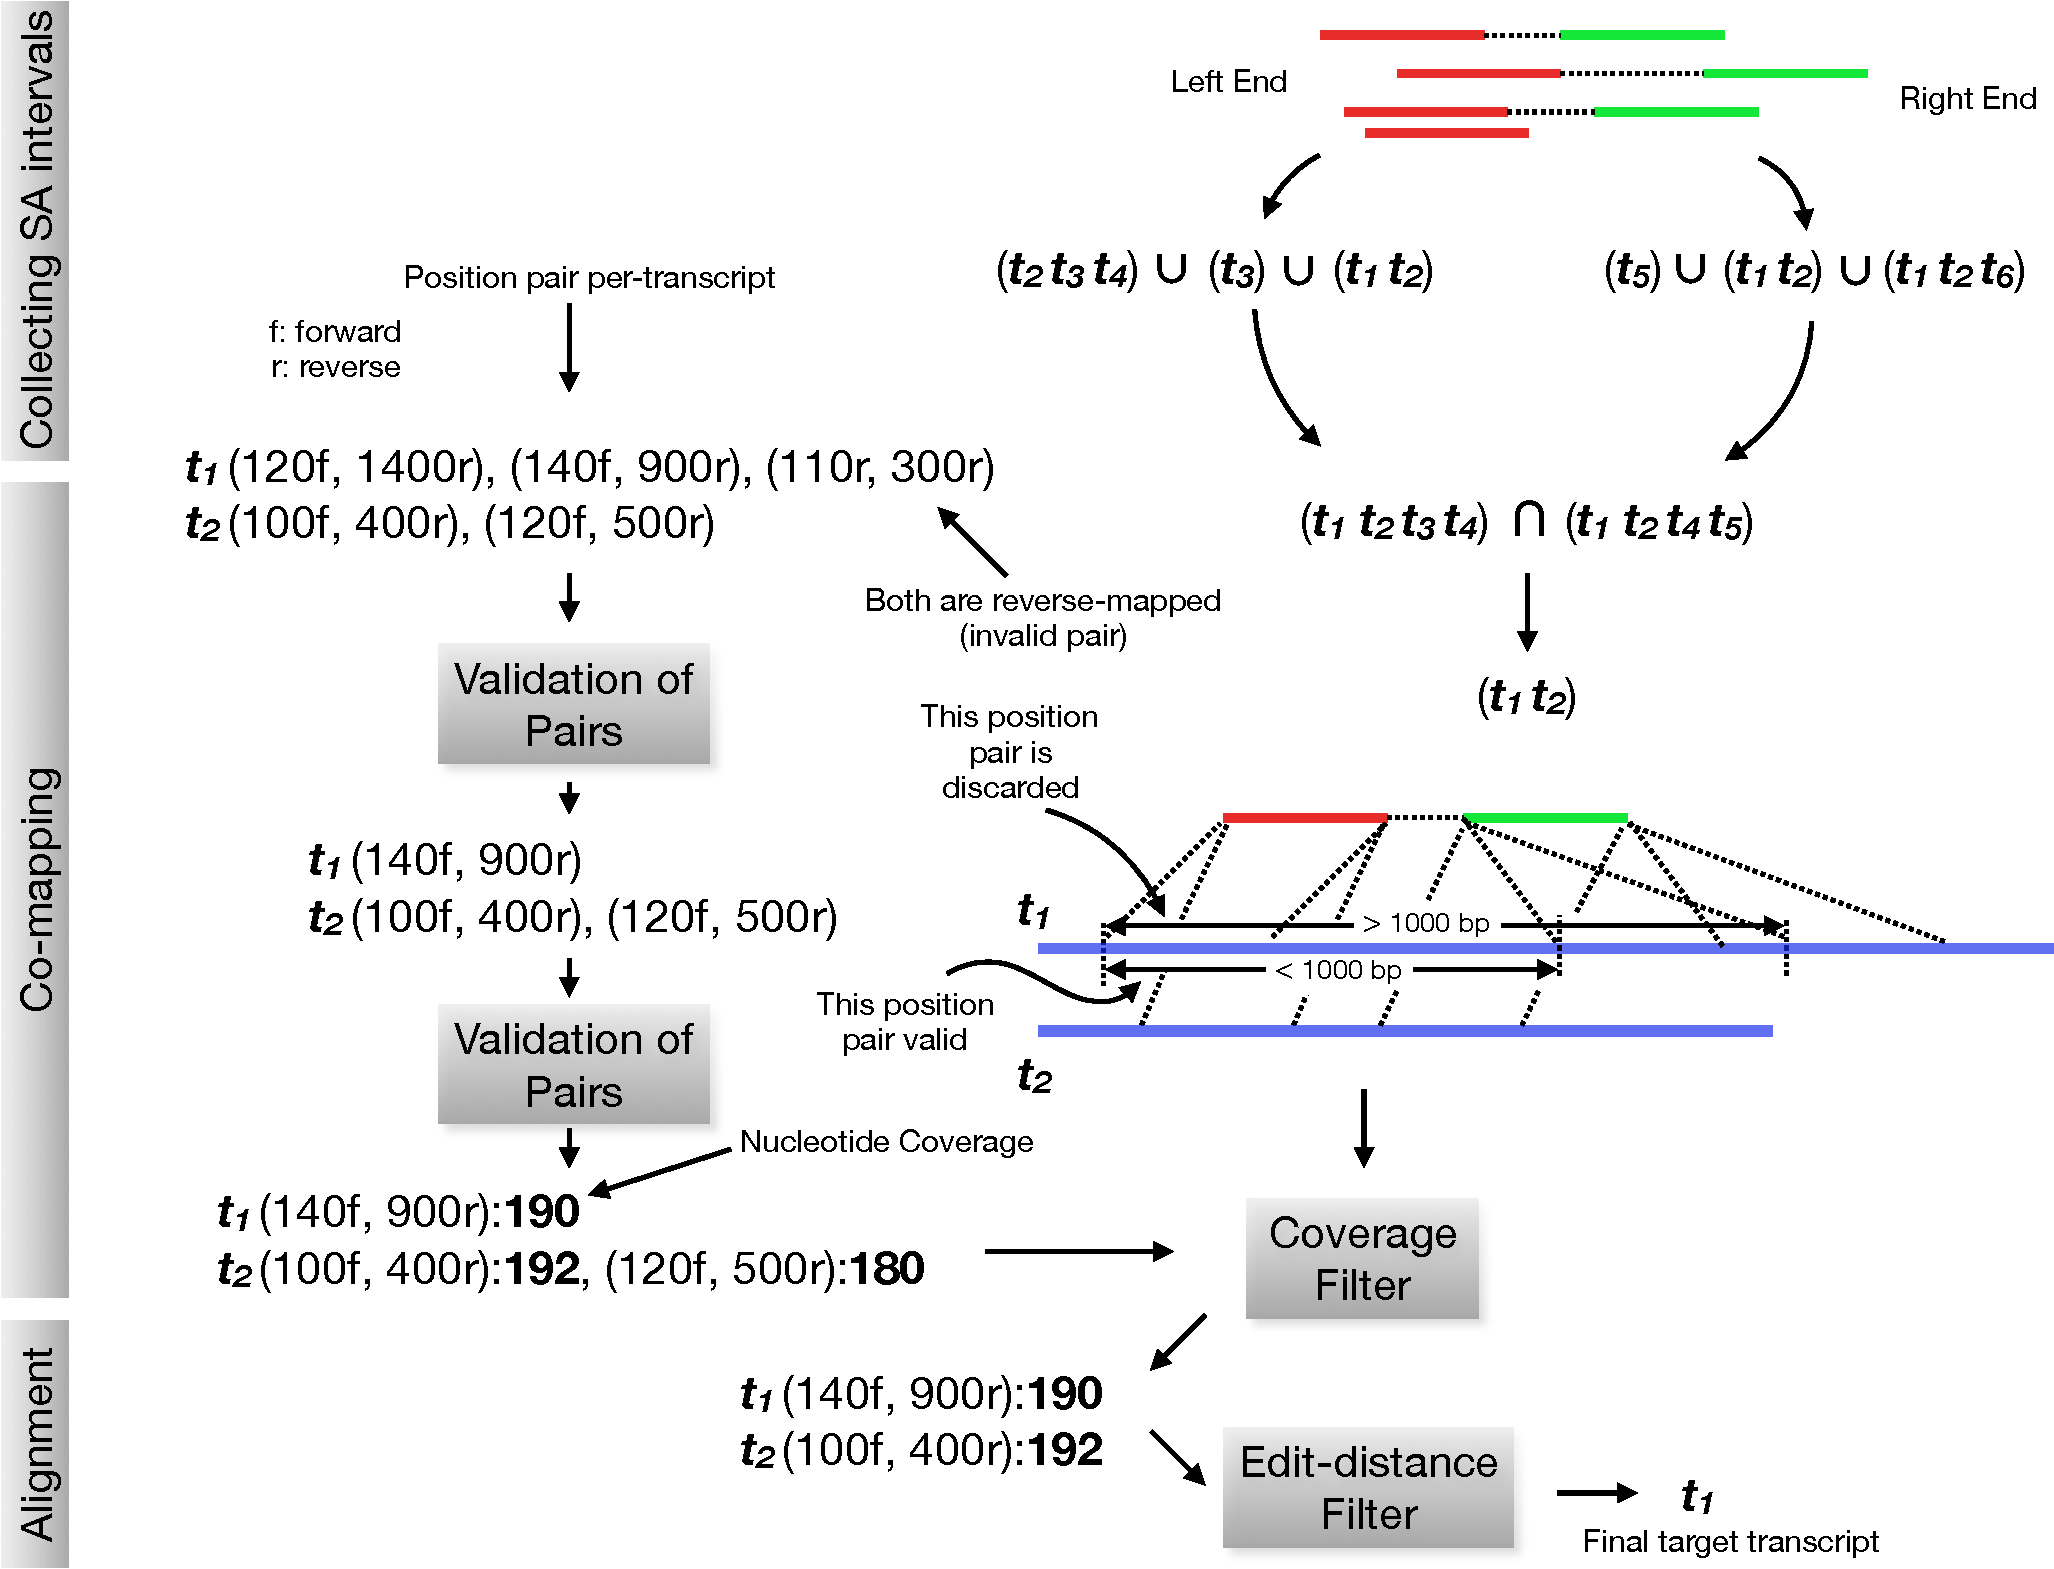
\includegraphics[scale=0.3]{Figures/sla/overview}
 \caption[The main steps of the \sla process]{The three main steps of the \sla 
 process are demonstrated here. First, suffix array ``hits'' are collected. Then, 
 in \cm, spurious mappings are removed by the orientation filter and then distance 
 filter. At most a single locus per-transcript is selected based on the coverage filter. 
 Finally, an edit-distance-based filter is used to select the valid target transcripts.
 }
  \label{fig:block_overview}
\end{figure}

\subsection{Defining and computing \kslcps}\label{sec:safelength}
Here, we formally define the concept of \kslcps (see figure~\cref{fig:safelength}). 
The determination of \kslcps starts by labeling each suffix array interval with the 
length of its corresponding longest common prefix and the associated transcript set it 
represents. Formally, $\LCP{\SuffixArray{[b]}}{\SuffixArray{[e-1]}}$ for an interval 
$\interval{b}{e}$ is the length of the common prefix of the suffixes $\SuffixArray{[b]}$ 
and $\SuffixArray{[e-1]}$. Given \kmer \samplekmer, where $\samplekmer \in \allkmers$ 
and \allkmers is the set of all \kmers from the reference sequence $T$, and the related 
interval $\ival{\samplekmer} = \interval{b}{e}$, for all $p \in \interval{b}{e}$, we 
consider each transcript $t$ such that the suffix $\SuffixArray{[p]}$ starts in transcript 
$t$ in the concatenated text. Then, for this interval, we can construct a set 
$\mathcal{C}^{\samplekmer} =  \{t_{i}, t_{j}, \dots\}$, which denotes the set of distinct 
transcripts that appear in the suffix array interval, indicated by \samplekmer.  We note 
that this notion discards duplicate appearances of the same transcript in this interval.

We compute the \kslcp for an interval indicated by \kmer $\samplekmer_i$ iteratively. The 
initial length for the \kslcp of the interval is $k$, length of a \kmer. We check, 
sequentially, each of the \kmers in the longest common prefix of the interval. For each 
new \kmer, the \kslcp is increased by one character. We terminate the \kslcp extension if 
any of the following conditions is encountered: (1) we reach the last \kmer contained 
in the LCP of this interval, (2) we encounter a \kmer $\samplekmer_j$ such that 
$\mathcal{C}^{\samplekmer_j} \not \subseteq \mathcal{C}^{\samplekmer_i}$ or (3) we 
encounter a \kmer $\samplekmer_j$ such that the reverse complement of $\samplekmer_j$ 
appears elsewhere in the transcriptome. When we encounter case (2) or (3), we call the 
\kmer $\samplekmer_j$ an \emph{intruder}.  That is, the \kmer will potentially alter our 
belief about the set of potential transcripts to which a sequence containing this \kmer 
maps (by strictly expanding this set), or the orientation with which it maps to the 
transcriptome.  We denote the \kslcp of a particular interval $\ival{\samplekmer_i}$ 
as $\mathrm{\texttt{\kslcp}}(\ival{\samplekmer_i})$.

As shown in figure~\cref{fig:safelength}, the \kslcp determination for the top suffix 
array interval starts with matching \kmers within the longest common prefix. The 
\kmer ``CAACG'' maps to a suffix array interval labeled with $(t_1,t_2)$. The next 
\kmer ``AACGG'', on the other hand, maps to a suffix array interval (shaded in green) 
labeled with $(t_1,t_2,t_3)$, thereby implying the \kslcp, shown as a dotted line. For 
each \kmer in the hash table, we store the length of the LCP and \kslcp, along with 
the corresponding suffix array interval.

\subsection{Discovering relevant suffix array intervals}
As shown in figure~\cref{fig:block_overview}, the selective-alignment approach can be 
broken into three major steps: collecting suffix array intervals, \cm, and selecting 
the high quality mappings. Gathering the suffix array intervals for a query read closely 
follows the \qm approach. It involves iterating over the read from left to right and 
repeating two steps. First, hashing a \kmer from the read sequence and then discovering the 
corresponding suffix array intervals. The process of \kmer lookup is aided by the \kslcp 
stored in the index (discussed in~\cref{sec:safelength}). The inbuilt lexicographic ordering 
of the suffixes in the suffix array, and the computed \kslcp values of intervals enable 
safely extending k-mers to longer matches without the possibility of masking 
potentially-informative substring matches. Given a matching \kmer, $\samplekmer_r$, 
from the read sequence $r$, we extend the match to find the longest substring of the 
read that matches within $\mathrm{\texttt{\kslcp}}(\ival{\samplekmer_r})$. The matched 
substring can be regarded as maximum mappable prefix (MMP)~\citep{Dobin2013Star}, that 
resides within the established \kslcp. We call this a maximal mappable safe prefix 
(MMSP --- eliding $k$ where implied). For a \kmer, $\samplekmer_r$, and interval, 
$\interval{b}{e}$, we note that $\mathrm{\texttt{\kslcp}}(\ival{\samplekmer_r}) 
\geq \length{\MMSP_{\samplekmer_r}}$, where $\length{\MMSP_{\samplekmer_r}}$ is the 
length of $\MMSP_{\samplekmer_r}$, the MMSP between the read's suffix starting with 
$\samplekmer_r$ and the interval $\ival{\samplekmer_r}$. The next \kmer lookup starts 
from the $(\MMSP_{\samplekmer_r}-k+1)$-th position. By restricting our match extensions 
to reside within the MMSP, we ensure that we will not neglect to query any k-mer that 
might \emph{expand} the set of potential transcripts where our read may map. We note 
here both the theoretical and practical relation between the \MMSP matching procedure, 
and the concept of a uni-MEM, as introduced by~\citet{debga}. The \kslcp for suffix array 
intervals are closely related to the lengths of unipaths in the reference de Bruijn 
graph of order $k$. Thus, our procedure for finding \MMSP{s}, that limits match 
extension by the \kslcp, is similar to the uni-MEM seed generation procedure described 
in debga \citep{debga}, with the distinction that in our method, we only consider extending 
seeds in one direction, and that we also choose not to terminate the \kslcp when the set 
of implied reference transcripts corresponding to the interval decreases in cardinality.

Given all the suffix array intervals collected for a read end (i.e. one end of a 
paired-end read), we take the \emph{union} of all the transcripts they encode. 
Formally, if  a read $r$ maps to suffix array intervals labeled with $\mathcal{C}^{r_1}, 
\ldots, \mathcal{C}^{r_n}$, then we consider all transcripts in the set $\mathcal{C}^{r_1} 
\cup \mathcal{C}^{r_2} \cup \ldots \cup \mathcal{C}^{r_n}$, and the associated positions 
implied by the suffix array intervals. As shown in~\cref{fig:block_overview}; 
this step is done before \cm.

We adopt a heuristic to avoid excessive \kmer lookups when we encounter a mismatch. 
When extension of an MMP is no longer possible, it is most probable that the mismatch 
results from an error in the read. If the mismatch is due to the presence of an error, 
then checking each \kmer overlapping this error can be a costly process. Instead, 
we move forward by a distance of $k/2$ in the read, and check the \kmer from the read 
such that the mismatch occurs in the middle position. If this \kmer lookup leads to 
another suffix array interval, we continue with the MMP extension process there; 
otherwise, we move again to the first \kmer that does not overlap this mismatch 
position. We observe that, in practice, the \kslcp, and hence the MMSP lengths can 
be quite large (\Cref{fig:dist}).

\subsection{Co-Mapping}
After collecting the suffix array intervals corresponding to left and right ends of the read, we wish to exploit 
the paired-end information in determining which potential mapping locations might be valid.  Hence, from this step 
onward, we use the joint information for determining the position and target transcripts. Given the suffix array 
intervals for individual ends of a paired-end read, the problem of aligning both ends poses a few challenges. 
First, a single read can map to multiple transcripts, and we wish to report all equally-best loci. Second, there 
can be multiple hits from a read on a single transcript (e.g., if a transcript contains repetitive sequence), and 
extra care must be taken to determine the correct mapping location. Finally, there may be hits that do not yield 
high-quality alignments (i.e. long exact matches that are nonetheless spurious).  To address the first and third 
points, we employ an edit distance filter to discard spurious and sub-optimal alignments.  To address the second 
challenge, we devise a consensus strategy to choose at most one unique position from each transcript.

Before applying the above mentioned strategy, we remove transcripts that do not contain hits from both the left 
and right ends of the read. Formally, given two ends of a read $r$, $r^{e_1}$ and $r^{e_2}$, and the corresponding 
suffix array intervals labeled with $\mathcal{C}^{r_1^{e_1}}, \ldots, \mathcal{C}^{r_n^{e_1}}$ and 
$\mathcal{C}^{r_1^{e_2}}, \ldots, \mathcal{C}^{r_m^{e_2}}$ respectively, we only consider transcripts present in 
the set $(\mathcal{C}^{r_1^{e_1}} \cup \ldots \cup \mathcal{C}^{r_n^{e_1}}) \cap (\mathcal{C}^{r_1^{e_2}} 
\cup \ldots \cup \mathcal{C}^{r_m^{e_2}})$.
We further refine this set by checking the validity of the alignments these hits might support. Currently, 
we use two validity checks illustrated in~\cref{fig:block_overview}. First, we apply an orientation-based 
check, and second, we employ a distance-based check. The orientation check removes potential mappings which have 
an orientation inconsistent with the underlying sequencing library type (e.g., both ends of a read mapping in the 
same orientation). The distance check removes potential alignments where the implied distance between the read 
ends is larger than a given, user-defined threshold ($1,000$ nucleotides by default).

\begin{figure}
 \centering
 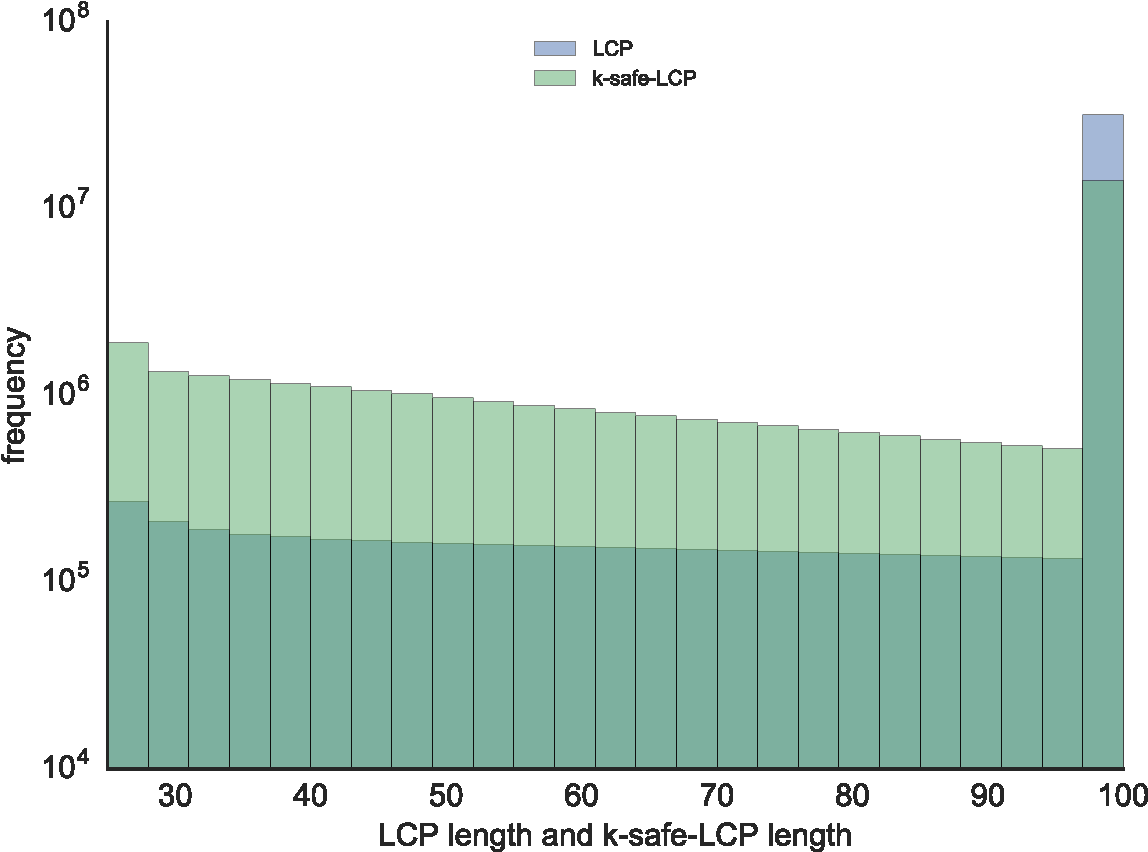
\includegraphics[scale=0.40]{Figures/sla/dist_safelength-color}
 \caption[The distribution of \kslcp lengths and LCP lengths]{The distribution of \kslcp lengths and LCP lengths 
 are similar and tend to be large in practice (human transcriptome).  Here, we truncate all lengths to a maximum 
 value of 100 (so that any LCP or \kslcp longer than 100 nucleotides is placed in the length 100 bin).}
\label{fig:dist}
\end{figure}

\begin{figure}
 \centering
 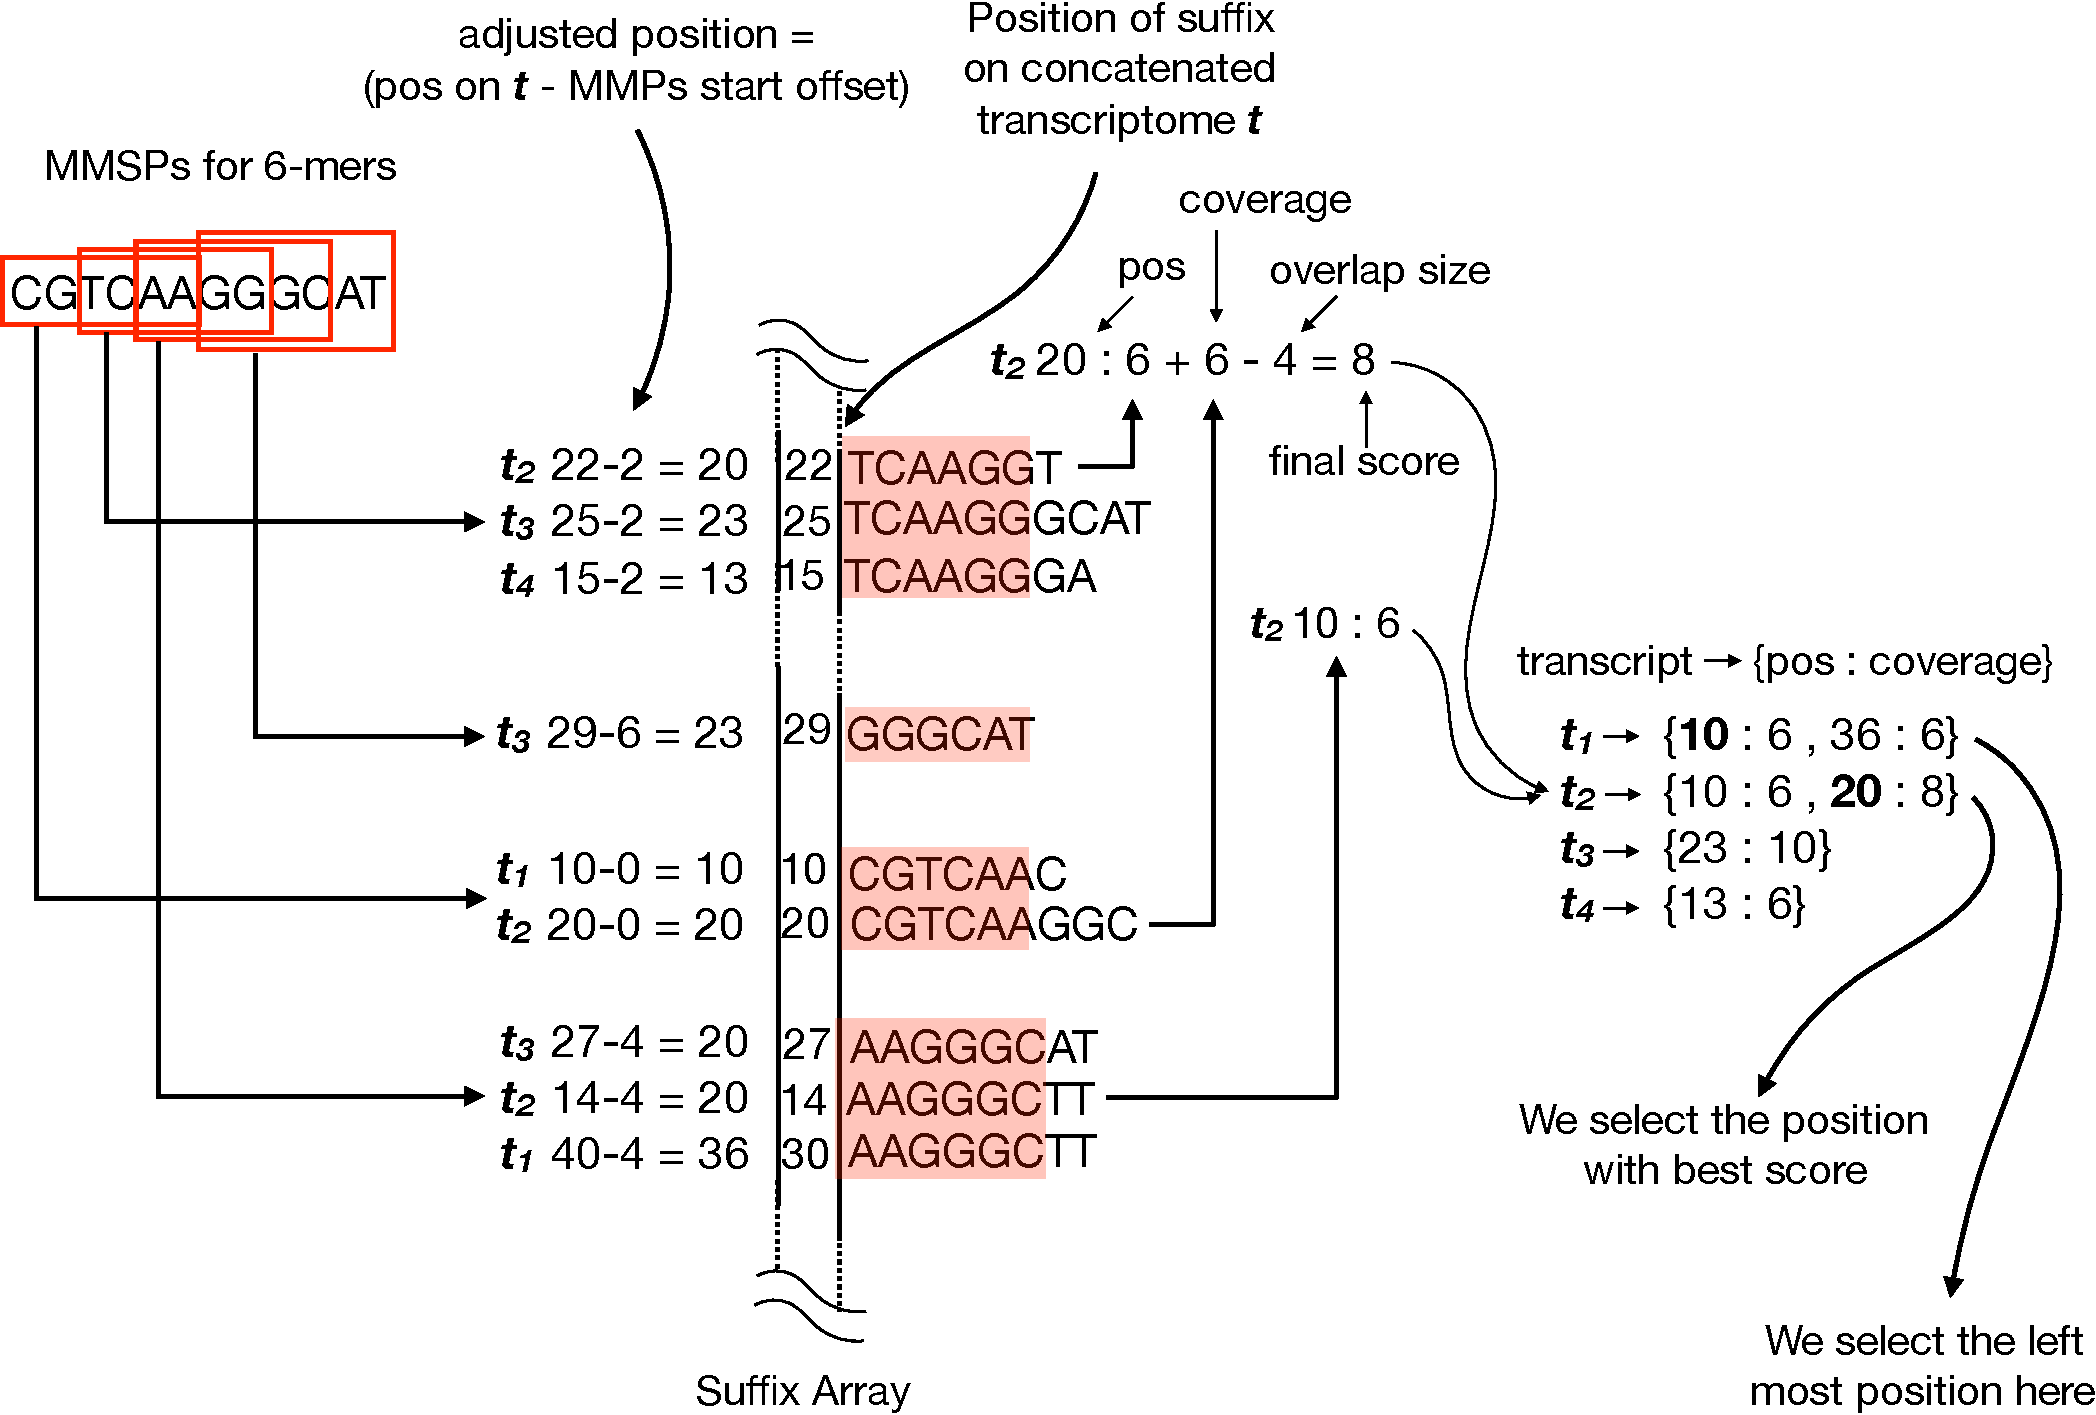
\includegraphics[scale=0.25]{Figures/sla/max_cov-color}
 \caption[Choosing the best postion on a transcript from multiple candidates]{The MMSPs corresponding to a read 
 are derived from multiple suffix array intervals. Here, all MMSPs happen to be of length $k$ as LCPs are of 
 size $k$. The coverage scheme finds out the exact positions on each transcript by adjusting the starting position of the MMSPs. The total score takes into account the positions where matches overlap. The final position is chosen by selecting the locus with maximum coverage.}
\label{fig:maxCov}
\end{figure}

\paragraph{Coverage based consensus:}
In \sla, the potential positions on a transcript are scored by their individual coverage on the target transcript.~\Cref{fig:maxCov} depicts the mechanism of choosing the best postion on a transcript from multiple probable mappings to the same transcript. The coverage mechanism employed in \sla makes use of the MMSP lengths collected during a prior step of the algorithm rather than simply counting \kmers. In~\cref{fig:maxCov}, the transcript $t_2$ has two potential mapping positions given the reads: position 10 and 20. The coverage consensus mechanism selects position 20 over position 10 due to the higher coverage by tiling MMSPs on the read.

\subsection{Selecting the best candidate transcripts}
Once the positional ambiguity within a transcript is resolved, the next step is selecting the best candidate transcripts from a set of mappings. Since mapping relies on finding exact matches, the length of the matched subsequence between the read and reference can sometimes be misguiding when comparing different candidate transcripts. That is, the transcripts with the longest exact matches do not always su A block diagram of the steps described below are depicted in Figure pport optimal alignments for a read.  At this point in our procedure, we follow the approach taken by many conventional aligners, and use an existing optimal alignment algorithm to compute the edit distance, by which we select the best candidate transcripts.

When performing alignment, we assume that a given read aligns starting at the position computed in the previous steps.  This helps us to reduce the search space within the transcript where we must consider aligning the read, and thereby considerably reduces the cost of alignment. To align the read at a specific position on the transcript and calculate the edit distance between them, we use $Myer's$ bounded edit distance bit-vector algorithm~\citep{myers1999fast}, as implemented in \texttt{edlib}~\citep{edlib}.  For a fixed maximum allowable edit distance, this algorithm is linear in the length of the read. We note that the bounded edit distance algorithm we employ will automatically terminate an alignment when the required edit distance bound is not achievable.

We remove all alignments with edit distance greater than a user-provided threshold. This is similar to the approach used by many existing aligners, and allows us to specify that even the best mapping for a given read may have too many edits to believe that it reasonably originated from a known transcript in the index. An appropriate threshold should be based on the expected error rate of the instrument generating the sequenced reads, and a very low threshold can lead to a decreased mapping rate.

\subsection{Enhancement of quantification accuracy based on edit distance}\label{filter}
We investigated the effect of incorporating edit distance in downstream quantification. Since we integrated the \sla scheme into the quantification tool \salmon \citep{Patro2017Salmon}, the edit distance scores from \sla can be used as a new parameter to \salmon{}'s inference algorithm.

%\mohsen{I modified some notations in the following paragraph, please verify if every thing is sound.}
In the framework of abundance estimation, we define the conditional probability of a generating a particular fragment, $f_j$, given that it comes from a specific transcript, $t_i$, as $P(f_j \mid t_i)$. Given the edit distance between the fragment and the transcript, we can incorporate this parameter into this conditional probability. \emph{Soft} filtering introduces a new term in the conditional probability based on $d_{i,j}$, which is the sum of the edit distances between the read ends of fragment $f_j$ and transcript $t_i$. We set this probability according to an exponential function, $P(a_{j}|f_j,t_i)=e^{-4d_{i,j}}$. The aggregate of threshold filtering and \emph{soft} filtering can be described as follows:\\

\begin{equation}
\Pr\left( a_{j} \mid d_{i,j}, \txp{i} \right)  =
      \begin{cases}
      0  & \text{$d_{i,j} > threshold$}\\
      e^{-4d_{i,j}}  &\text{$d_{i,j} \le threshold$}
      \end{cases}.
  \label{eqn:softFilter}
\end{equation}

\paragraph{Preventing redundant alignments by exploiting shared LCPs:}\label{sharedLCP}
Exploiting the common subsequences in the transcriptome is instrumental to the superior speed of fast mapping, 
\nab tools. Reads generated from exonic sequences common to multiple transcripts from the same gene or paralogous 
genes are the main source of ambiguous mappings. As we rely on the suffix array data structure to obtain the 
initial set of transcripts to which a read maps, there are cases where exactly identical reference sequences 
all act as mapping targets for the read. For a suffix array interval $\interval{b}{e}$, we identify such common 
subsequences by examining the {\it longest common prefix} (LCP) of the interval. If the length of the LCP is 
equal or greater than the length of the read, then the actual alignment against the underlying reference at 
these positions will be identical. We observed that for almost half of the read-transcript pairs, the alignment 
process can be avoided. Note that if the read sequence shares a complete match with the common prefix, meaning 
that maximum mappable safe prefix length is equal to read length (i.e., the read matches the reference exactly 
at some set of positions), we can also bypass the Meyer's edit distance algorithm call completely.

\paragraph{Avoids redundant work by caching alignment sub-problems further:} We also extend a similar idea to the 
scenario where only part of the reference sequence is shared between references.  Specifically, when performing an 
alignment between anchoring exact matches, we store the result in a hash table where the key is a tuple 
$\left(i,j,h\left(i', j'\right)\right)$ and the associated value is the computed edit distance.  Here, $i$ 
and $j$ denote the start and end of the read interval being aligned and $i'$ and $j'$ denote the start and 
end of the reference sequence; $h(i',j')$ is a hash of the corresponding reference sequence 
(we use \texttt{xxhash}~\citep{xxhash}).  This allows us to detect when a redundant alignment sub-problem for 
a read is shared between references, and to reuse the cached result in such cases.


\subsection{Evaluating the performance of \sla}


To evaluate the effectiveness of \sla, we coupled it with the quantification tool \salmon (branching from the v0.9.1 
release). This enables us to measure the effect of different alignment based and non-alignment based algorithms on 
transcript-level quantification results directly, holding the statistical estimation procedure fixed. We also include 
\kallisto(v0.43) in our benchmarks, which provides a perspective on \pa-based quantification. Furthermore, we compare 
the performance of \sla with the recent, fast, hashing and alignemnt-based, abundance estimation tool (currently un-published) 
\hera~\footnote{\url{https://github.com/bioturing/hera}}. We note, this is an early version of the \hera(v1.2) software, 
which is already performing very well in our testing, but is subject to changes and improvements. Given it's impressive 
performance (in both time and accuracy), we decided to include \hera in our comparisons with the consent of its authors 
(personal communications). We measure the Spearman correlation and Mean Absolute Relative Differences (MARD) of read 
counts as performance metrics when comparing the different methods.
%(further metrics are also provided for some of the experiments in the supplementary material). 
All experiments of this section were performed on an Intel(R) Xeon(R) CPU (E5-2699 v4 @2.20GHz 
with 44 cores and 56MB L3 cache) with 512GB RAM and a 4TB TOSHIBA MG03ACA4 ATA HDD running ubuntu 16.10 and each method 
was run using 16 threads.

In all our experiments, reads are mapped to the transcriptome using using \bt, \kallisto, \hera, \sla and \STAR. 
Subsequently, transcripts are quantified by \salmon(v0.9.1) using the relevant mappings (from alignment or the 
\nab methods) as input (except in the cases of \kallisto(0.43) and \hera(1.2), which include implementations of 
their quantification algorithms). The alignment mode of \salmon enables us to use \STAR(v2.5) and \bt(v2.3) output 
as a direct input to the quantification module --- thereby reducing variability due to differences in the 
underlying methodology used for quantification. To achieve the most sensitive alignment, \bt is run with the 
alignment options suggested for use with \rsem~\citep{rsembmc}. For aligning reads to the transcriptome using 
\STAR, we used the same options described in \citep{Srivastava2016rapmap}. When processing alignments, \salmon 
was run with \texttt{-{}-rangeFactorizationBins 4}~\citep{ismb2017factorization} and \texttt{-{}-useErrorModel}. 
With \sla, \salmon was run using the \texttt{-{}-softFilter} flag (discussed in~\cref{filter}), 
a range factorization value of 4 and an edit distance threshold of 7. \kallisto was run with default parameters. 
Both the \sla and \kallisto indices were built with $k=25$; \hera does not include \kmer size as a user-defined 
parameter.

\subsection{Quantification of simulated reads against mutated transcriptomes}\label{subsec:synthetic}

We explored the performance of different alignment-based and alignment-free methods by quantifying simulated short 
RNA-seq reads against mutated reference sequences. The simulation process consists of two steps. In the first step, 
we mapped an experimental RNA-seq sample (accession number SRR5638585) to the human transcriptome (Ensembl release 
80 \citep{yates2015ensembl} ) using \salmon. The resulting abundance vector, in conjunction with the full 
transcriptome sequence generated from the full human genome and the corresponding annotations (version GRCh37.p13), 
is used to simulate five batches of 100bp paired-end RNA-seq samples, where each batch contains $\sim47$M reads. 
We used the sequence simulator Polyester \citep{frazee2015polyester} for generating the read datasets.

While the simulated dataset enables comparison with the ground truth, the quality of the reads is high and does 
not show the subtle nuances that arise when mapping reads from experimental sequencing datasets. In reality, the 
sequenced reads could differ from the annotated reference sequence due the presence of mutations (variants) in the 
sequenced organism. In other cases, a reference sequence from one species could be used to analyze data from a 
phylogenetically closely related species, for which an annotated reference in unavailable. Therefore, to 
recapitulate these adversarial situations, instead of mapping the simulated reads to the exact underlying 
transcriptome used for read generation, we map them against references mutated at a controllable rate.

The mutated version of the transcriptome is derived from the underlying reference genome that was subject to 
random mutations. The nucleotides of the reference genome were randomly altered based on a Poisson process with 
a tunable {\it rate} parameter. The rate parameter enables controling the rate of mutation that we want to 
introduce in the reference genome. For the current manuscript we have used $5$ equally spaced rate parameters 
from $0.01$ to $0.05$. The mutated genome sequences and the original annotation are used to generate the mutated 
reference transcriptomes. As the resulting transcriptomes contain devations from the indexed reference, we believe 
that mapping to these references will capture some aspects of the difficulties encountered when applying such tools 
to certain experimental datasets.

To evaluate the performance we have measured the quantification accuracy of different tools with respect to the 
ground truth provided to Polyester. As explained earlier, tools such as \kallisto, \hera and \sla have a 
quantification pipeline attached to the mapping module and are, therefore, capable of generating abundance 
vectors directly. On the other hand, \bt and \STAR generate alignment files that we have coupled with \salmon 
(run in alignment-based mode) to obtain abundance estimates.

\begin{figure}
 \centering
 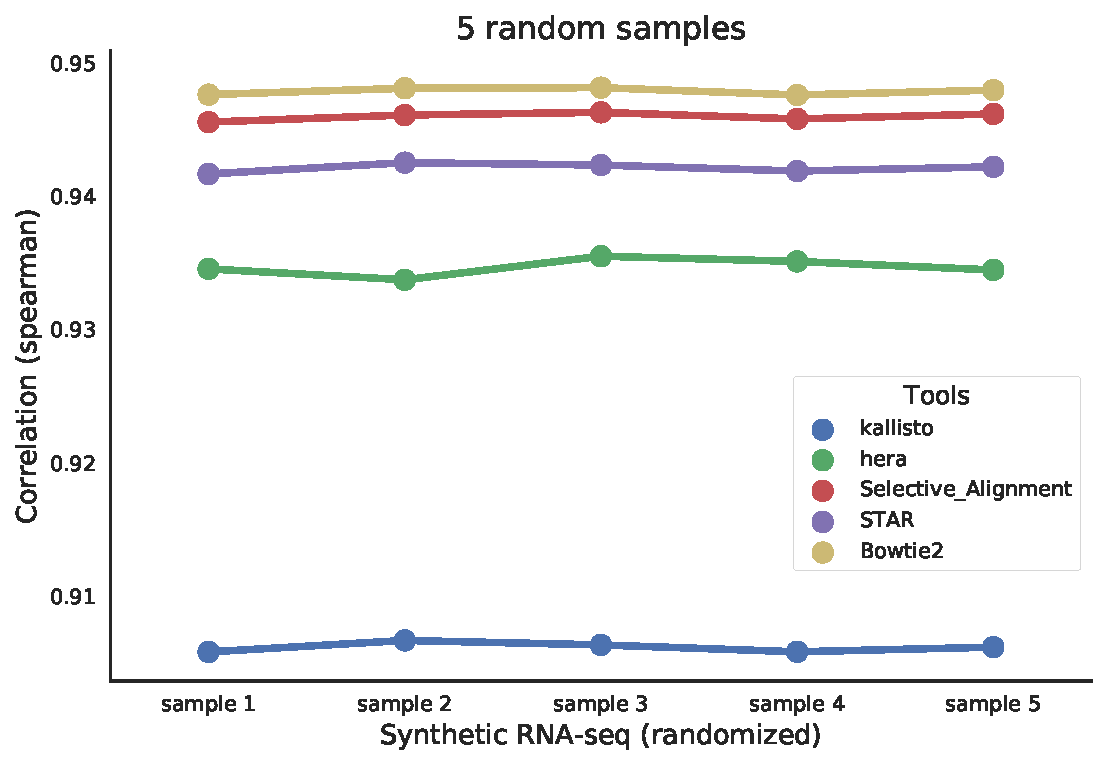
\includegraphics[scale=0.40]{Figures/sla/standard_error}
 \caption[Performance of tools on paired end reads]{Performance variation of 
 different tools on paired end reads produced with five random seeds.}
  \label{fig:random_samples}
\end{figure}

Performance of the various methods on a simulated sample is shown in~\cref{tab:diff_mutation_sp}
and~\cref{tab:diff_mutation_mard}. In this case, 
the simulated sample is mapped against $5$ different mutated transcriptomes with increasing error rates and the 
corresponding spearman correlation and MARD values calculated using the ground truth. As shown in 
\cref{tab:diff_mutation_sp}, the correlation between quantification estimates using \sla and the ground truth is 
higher than the other self-contained quantification methods, \kallisto and \hera. This gap between correlation 
values increases as the rate of mutation in the reference transcriptome is increased, showing the ability of 
\sla to accurately map reads against diverging transcriptomes. The MARD values for \sla are lower in comparison 
with other \nab methods as well.

To measure the variation in quantification about a single random instance of simulated data (i.e., data generated 
with a particular random seed), we have also generated five different simulated RNA-seq datasets by passing 
different seeds to Polyester. To minimize external variation, we used the least mutated transcriptome 
(rate 0.01) as reference. By plotting the spearman correlations, as shown in~\cref{fig:random_samples}, 
we observe that, given that all the tools perform well on the random samples, the performance of \sla is grouped 
with the alignment-based methods, such as \bt and \STAR.  Further, the variation in quantification performance of 
all methods (i.e. the standared error) across these different simulated replicates is very small.

\begin{table}
\begin{center}
\begin{tabular} {c|c c c c c}
\toprule
  Mutation Rate & Kallisto & Hera & Selective Alignment & STAR-Salmon &Bowtie2-Salmon \\
\midrule
  0.01 & 0.906 & 0.935 & \textbf{0.946} & 0.942 & \textbf{0.948} \\
  0.02 & 0.871 & 0.925 & \textbf{0.942} & 0.939 & \textbf{0.945} \\
  0.03 & 0.844 & 0.910 & \textbf{0.935} & 0.933 & \textbf{0.942} \\
  0.04 & 0.817 & 0.880 & \textbf{0.925} & \textbf{0.925} & \textbf{0.937} \\
  0.05 & 0.793 & 0.845 & 0.904 & 0.909 & \textbf{0.927} \\
\bottomrule
\end{tabular}
\caption[Acuracy of qunatification of synthetic dataset against the mutated reference transcriptome]{
  {Synthetic dataset quantified against the mutated reference transcriptome with different mutation rates. 
  The spearman correlation is calculated with respect to the ground truth.}
}
\vspace{-0.3in}
\label{tab:diff_mutation_sp}
\end{center}
\end{table}

\begin{table}
\begin{center}
\begin{tabular} {c|c c c c c}
\toprule
Mutation Rate & Kallisto & Hera & Selective Alignment & STAR-Salmon &Bowtie2-Salmon \\
\midrule
  0.01 & 0.161 & 0.116 & \textbf{0.100} & 0.104 & \textbf{0.096}\\
  0.02 & 0.193 & 0.132 & 0.108 & 0.109 & \textbf{0.100}\\
  0.03 & 0.215 & 0.172 & 0.120 & 0.115 & \textbf{0.107}\\
  0.04 & 0.236 & 0.231 & 0.143 & 0.127 & \textbf{0.118}\\
  0.05 & 0.257 & 0.291 & 0.186 & 0.150 & \textbf{0.142}\\
\bottomrule
\end{tabular}
\caption[MARD of qunatification of synthetic dataset against the mutated reference transcriptome]{
  {Synthetic dataset quantified against the mutated reference transcriptome with different mutation rates. 
  The MARD (mean absolute relative difference) is calculated with respect to the ground truth.}
}
\vspace{-0.3in}
\label{tab:diff_mutation_mard}
\end{center}
\end{table}


\subsection{Experimental reads from human transcriptome}\label{res:experimental}

We have also benchmarked our proposed \sla method on experimental data from SEQC(MAQC-III) 
consortium ~\citep{seqc2014comprehensive} samples (SRA accession \texttt{SRR1215996} - \texttt{SRR1216000}). 
Each of the five technical replicates consists of $\sim$11M$, 100$bp, paired-end reads, sequenced on an 
Illumina Hiseq 2000 platform.

We follow the same basic assessment methodology as discussed in~\cref{subsec:synthetic}, and report the mean 
Spearman correlation and MARD value for each method. However, we note that, since this is experimentally-derived 
data, there is no knowledge of ground truth transcript abundances.  Instead, we have measured the overall 
concordance between different approaches. Given the results obtained in all of our other testing, we expect 
the \bt-based pipeline to be the most accurate, so we are generally looking for high concordance with those 
quantifiaction estimates.

In~\cref{tab:correlations}, we compare the quantification results produced by different methods. Each 
individual cell contains the average obtained across the five samples. High Spearman correlation and low MARD 
value between \bt and \sla show that \sla produces results most similar to those based on \bt. Interestingly, 
the concordance between the \sla and \bt-based pipelines is even higher than the concordance between the two 
pipelines based on more traditional alignment approaches (i.e. \bt and STAR). While we cannot assess the accuracy 
with respect to known ground truth on these samples, we nonetheless believe assessments based on real data like 
this are important to perform, as the complexity of experimental data seems to be considerably higher than that 
of simulated data and its characteristics can be markedly different. Finally, \Cref{tab:experimental_timing} 
provides timing and memory assessments of all the methods running on sample \texttt{SRR1215996}. Since the 
mapping phase of \sla is not distinct from the quantification phase, the memory and time footprints include 
the mapping part of the pipeline.  Further, disk space is not comparable to alignment-based methods, since 
alignment files are not written directly as output of \sla (rather, the \sla algorithm informs the mappings 
and provides edit-distance-based scores --- as described in~\cref{eqn:softFilter} --- directly to the 
quantification algorithm).

\begin{table}
\renewrobustcmd{\bfseries}{\fontseries{b}\selectfont}
\sisetup{detect-weight,mode=text,group-minimum-digits = 4}
\centering
\begin{tabular}{|l|c|c|c|c|c|}
\hline
 Method & \kallisto &\hera  & selective & \STAR & \bt \\ %& \qm
\hline
\kallisto &  \diagbox[]{\num{1}}{\num{0}} & \num{0.189293544242057} 
& \num{0.160148930794467} & \num{0.152536064490726} & \num{0.168211319115239} \\
\hline
\hera & \num{0.868172058407572} & \diagbox[]{\num{1}}{\num{0}} 
& \num{0.134994519090086} & \num{0.147176566236675} & \num{0.137529630659189}\\
\hline
\ssla & \num{0.898126618322603} & \num{0.902170309453134} & \diagbox[]{\num{1}}{\num{0}} 
& \num{0.128558965365635}   & \ubold \num{0.0585736425878761}\\
\hline
\STAR &   \num{0.898360010715753} & \num{0.89565317161376} & \num{0.912909527305415} 
& \diagbox[]{\num{1}}{\num{0}} & \num{0.128710771202473} \\
\hline
\bt & \num{0.890488189578628} & \num{0.900958882919405} & \ubold \num{0.966015219762142} 
& \num{0.913252923042169} & \diagbox[]{\num{1}}{\num{0}} \\   \hline
\end{tabular}
\caption[The accuracy of quantifications computed by all methods on experimental data]
{The Spearman correlation and MARDS between transcript abundances computed by all methods on 
experimental data. Each number is the mean on 5 different samples; the numbers in the lower 
left triangle of the matrix are the Spearman correlations and the ones in upper right are 
the MARD values. "\ssla" refers to \sla.}
\label{tab:correlations}
\end{table}

\begin{table}%[h]
\centering
\begin{tabular}{lrr}
\toprule
Method &time (s) & memory (KB) \\
\midrule
\kallisto & \num{61} & \num{4006284} \\
\hera  & \ubold \num{38} & \num{6736576} \\
\sla & \num{65} & \num{7994324} \\
\STAR & 398+96 & max(\num{8342444},\num{5513432}) \\
\bt & 977+125 & max(\num{1020032},\num{9949380}) \\

\bottomrule
\end{tabular}
\caption[Comparison of timing and memory foot-print of \sla with other alignment and non-alignment methods]
{Comparison of timing and memory foot-print of \sla with other alignment and non-alignment methods 
on experimental sample SRR1215996. The timing performance for \STAR and \bt is the sum of mapping 
and quantification (with salmon) steps (first number is the mapping step) and memory footprint is 
the max memory footprint of these two steps (first number is for the mapping step).\\}
\label{tab:experimental_timing}
\end{table}

\subsection{Conclusion}
Recently, fast \nab approaches have been developed for mapping RNA-seq reads to transcriptomes. Rather than 
generating full alignments, these approaches compute ``mapping'' information that is often sufficient for 
a number of  given analysis tasks (e.g., transcript 
quantification~\citep{Patro2014Sailfish,zhang2014rna,Bray2016Kallisto,Patro2017Salmon,ju2017fleximer} 
or metagenomic abundance estimation~\citep{Schaeffer2017}). Yet, there exist scenarios where such \nab approaches 
can go awry; either failing, by the greedy nature of their procedures, to find the true target of origin of 
a read, or by allowing spurious mappings to targets supported by exact matches that would nonetheless fail 
reasonable alignment scoring filters. Moreover, it is sometimes desirable to be able to produce, on demand, 
the edit distance or alignment that would result from a given mapping location. The recently-introduced \hera 
validates mapping quality using alignment, which resolves spurious mappings, though it still suffers a loss of 
sensitivity compared to traditional alignment methods, and fails to process \denovo assembled transcriptomes. 
In this section, we introduced a selective alignment algorithm that attempts to bridge the gap between these \nab 
algorithms and more traditional alignment approaches. \Sla improves upon both the sensitivity and specificity 
of these \nab algorithms while making very moderate concessions with respect to the computational budget. 
To achieve this level of efficiency, a number of algorithmic innovations were required, some of which may be of 
general interest. In the future, we hope to expand upon the notion of selective alignment even further, both by 
improving the algorithm and implementation, and by exploring use cases where selective alignment applies. Such 
situations are those where fast \nab approaches are inappropriate and traditional alignment approaches are too 
slow. In terms of improving the method, we hope to add functionality to automatically predict the optimal edit 
distance threshold in the read mappings based on the quality of the alignments, and for \sla to self-tune to 
properly handle edge cases, such as soft clipping. The \sla algorithm currently implements user specified edit 
distance threshold for filtering spurious reads. A more data-driven choice of filter can lead to a more resilient 
threshold that can perform gracefully while handling both adversarial reads as well as high-quality reads in 
heterogeneous read samples. In high quality samples, the edit distance bound can be set lower to further 
speed-up the algorithm. Future work will also include support for reporting the actual CIGAR strings for 
applications that require this information, such as RNA-seq based variant calling or allele identification.

\section[Puffaligner]{Puffaligner: An efficient and accurate aligner based on the pufferfish index}
Short-read aligners are a major workhorse of modern genomics. Given the importance of the alignment problem, 
a tremendous number of different tools have been developed to tackle this problem. Some widely used examples are
\bwa~\citep{bwa}, \bt~\citep{bowtie2}, \hisat~\citep{hisat,hisat2} and \st~\citep{star}.
Existing alignment tools use a variety of indexing methods. Some tools, such as \bwa, \bt, and \st
use a full-text index over the reference sequences; \bwa and \bt use variants of the FM-index, 
while \st uses a suffix array.

A popular alternative approach to full-text indices is to instead, index sub-strings of length $k$ (\kmers) 
from the reference sequence. Trading off index size for potential sensitivity, such indices can either index
all of the \kmers present in the underlying reference, or some uniform or intelligently-chosen sampling of \kmers. 
There are a large variety of \kmer-based aligners, including tools like the Subread
aligner~\citep{subread}, SHRiMP2~\citep{shrimp2}, mrfast~\citep{mrfast}, and mrsfast~\citep{mrsfast}. 
To reduce the index size, one can choose  to select specific \kmers based on a winnowing (or minimizer) scheme.
This approach has been particularly common in tools designed for long-read sequence alignment like 
mashmap~\citep{Jain2018} and minimap2~\citep{minimap2}.

Recently, a set of new indices for storing \kmers have been proposed based on graphs, specifically \dbgs (\dbgshort). 
A \dbg is a graph over a set of distinct \kmers where each edge connects two neighboring \kmers
that appear consequently in a reference sequence and therefore, overlap on ``$k-1$'' bases. \kallisto~\citep{kallisto}, 
\debga~\citep{debga}, BGreat~\citep{bgreat}, \brownie~\citep{brownie}, and \pufferfish~\citep{pufferfish} are some
tools which use an index constructed over the \dbg built from the reference sequences. 
Cortex~\citep{cortex}, Vari~\citep{vari}, rainbowfish~\citep{rainbowfish}, and mantis~\citep{mantis} are also tools
that use a \ccdbg for building their index over a set of raw experiments. All these approaches cover a wide range 
of the possible design space, and different design decisions yield different performance tradeoffs.

Generally, the fastest aligners (like \st) have very large memory requirements for indexing, and make 
some sacrifices in sensitivity to obtain their speed. On the other hand, the most sensitive aligners (like
\bt) have very moderate memory requirements, but obtain their sensitivity at the cost of a higher runtime. 
Maintaining the balance between time and memory is especially more critical while aligning 
to a large set of references, like a large collection of microbial  and viral genomes which may 
be used as an index in microbiome or metagenomic studies. As both the collection of reference genomes and 
the amount of sequencing data grows quickly, it is import for alignment tools to achieve a time-space balance 
without loosing sensitivity.

Based on the compact \pufferfish~\citep{pufferfish} index, we introduce a new aligner called \puffaligner,
that we believe strikes an interesting and useful balance in this design space. \puffaligner is designed 
to be a highly-sensitive alignment tool while, simultaneously, placing a premium on computational overhead.
By using the \ccdbg to factor out repeated sub-sequences in the reference, it is able to leverage the speed 
and cache friendliness of hash-table based aligners while still controlling 
the growth in the size of the index; especially in the context of redundant reference sequences. By carefully 
exploring the alignment challenges that arise in different assays, including single-organism DNA-seq, 
RNA-seq alignment to the transcriptome, and metagenomic sequencing, we have engineered a versatile
tool that strikes desirable balance between accuracy, memory requirements and speed. We compare 
\puffaligner to some other popular aligners and show how it navigates these different tradeoffs. 
\puffaligner is a free and open-source software and it is implemented in C++14 and can be obtained 
from \url{https://github.com/COMBINE-lab/pufferfish/tree/cigar-strings}.

\subsection{Main pipeline in \puffaligner}
\puffaligner is an aligner built on top of the \pufferfish indexing data structure. \pufferfish is a 
space-efficient and fast index for the \ccdbg (\ccdbgshort). A \ccdbg is a graph whose vertices
(strings) are the compacted non-branching paths of the underlying \dbg, with the restriction that 
each node also have the same color set (set of reference sequences in which it appears). The nodes in the
\ccdbg are referred to as \unitigs. Each \unitig can be mapped to a list of $<$reference ID, position, 
orientation$>$ tuples that describe exactly how this subsequence appears in the unlderying
collection of references. The basic query operation in the \pufferfish index is to query 
a \kmer from the input sequence against the index. Given this query, the pufferfish index returns the unique
position (and orientation) where this \kmer appears in the \ccdbg (or  a sentinel value if this \kmer 
does not occur). This match between the query and the graph can then be easily ``unpacked'' into the implied list of 
matches with the underlying references by finding all of the places that the  matched \unitig appears in the 
reference sequences and translating the relative position within the unitig into the corresponding 
reference position (and adjusting the orientation if necessary). The output of this step is then a list of all 
of the reference sequences, positions, and orientations where this exact match occurs.  While \kmer query is the 
basic operation performed by the index, we actually do not use \kmer matches  directly, and instead 
extend the initial match into unique maximal exact matches (uni-MEMs).

Specficially, each \kmer match is extended simultaneously in both the  query and reference to 
obtain a longer exact match. The exact matches to the unitigs, called \unimems, are then projected to
the positions on the references associated to that \unitig. Then, \unimems  are aggregated into MEMs 
(described below) on each reference, and the chains of MEMs with the highest score are selected. 
In the case of paired-end reads, the chains of the left and right ends are paired with respect to their distance,
orientation, etc. Finally, rather than fully aligning each query sequence to the anchored position 
on the reference, only the sub-sequences from the query that are not part of the \unimems (exact
matches) are aligned to the reference; we call this procedure the between-\mem alignment. Each of 
these steps are explained in detail in the following sections.

\subsection{Exact matching in the \pufferfish index}

The pufferfish index provides \puffaligner with an efficient index for \kmer lookup within a list of references. 
Specifically, the core components of the index are (1) a minimal perfect hash function (MPHF), (2) a \unitig 
sequence vector, (3) a \unitig-to-reference table, and (4) a vector storing the position associated with each
\kmer in the \unitig sequence vector. The \unitig sequence vector contains all the \unitigs in the 
\ccdbgshort. The \pufferfish index admits efficient exact search for \kmers, as well as longer matches
that are unique in both the query string and \ccdbg. These matches, called \unimem, were originally 
defined in \debga~\citep{debga}. A \unimem is a Maximal Exact Match (\mem) between the query sequence
and a \unitig. Using the combination of the MPHF and the position vector, a \kmer is mapped to a \unitig 
in the \unitig sequence vector. The \kmer is then extended to a \unimem via a linear scan 
of the query sequence and the \unitig sequence vector. Each \unimem can appear  in multiple different references, 
and since \unimems must be completely contained within a \unitig, it is possible for multiple 
\unimems to be directly adjacent on both the query and some references where the \unitig appears.

\paragraph{\unimem collection:}
The first step in read alignment is to collect exact matches shared
between the query (single-end or paired-end reads) and the reference.
In \puffaligner, this is accomplished by collecting the set of
\unimems that co-occur between the query and reference. \puffaligner
starts processing the read from the left-end and
looks up each \kmer that is encountered until a match to the index is
found. Once a match is discovered, it is extended in both query and the reference 
%\rob{do we actually extend in both directions, or just one?} 
until one of these termination conditions occur: (1) a mismatch is encountered, 
(2) the end of the query is reached, or (3) the end of the
\unitig is reached. This process results in a \unimem match shared
between the query and reference. \unimems where extension is terminated
as a result of reaching the end of a \unitig must later be 
examined and potentially ``collpased'' together to form MEMs with respect
to the references on which they appear. If the \unimem extension is not
terminated as a result of reaching the end of the query, then the
position in the read is incremented by a small value and the same procedure is repeated
for the next \kmer on the read. This process continues until either
the \unimem extension terminates because the end of the query is
reached, or because the last \kmer of the query is searched in the index.
Here, we recall an important property of \unimem extension that is
different from e.g. \mem extension or maximum mappable prefix (MMP)
extension~\citep{star}. Due to the definition of the \ccdbgshort, it
is guaranteed that any \kmer appearing within a \unimem cannot appear
in any other unintig in the \ccdbgshort. Thus, extending \kmers to
maximal \unimems is, in some sense, safe with respect to greedy
extension, as such extension will never cause missing a \kmer that
would lead to another distinct \unimem shared between the query and
reference. The concept of safe extension of kmer matches was introduced in~\citep{selaln}.

\paragraph{Filtering highly-repetitive \unimems:}
\label{par:repetitivehits}
In order to avoid expending computation on performing the subsequent
steps on regions of reads mapping to highly-repeated regions of the
reference, any \unimem that appears more than a user-defined number
of times in the reference is discarded. In this manuscript, we use
the threshold of $1000$. This filter has a strong impact on the
performance, since, even if one \kmer from the read maps to a
highly-repetitive region of the reference, the following expensive
steps of the alignment procedure should be performed for every
mapping position of the \unimem to find the right alignment for the
read, while the less repetitive \unimems also map to the true origin
of the read on the reference as well. The drawback of this filter is that
for a very small fraction of the reads which are truly originating
from a highly-repetitive region, all of the matched \unimems will be
filtered out and no hit remains for aligning the read. However,
we find that in the case of aligning paired-end reads, usually one
end of the read maps to a non-repetitive region, then, the alignment
of the other end can be recovered using orphan recovery (explained
in~\Cref{subsec:orphan_recovery}). Futheremore, we also provide 
a flag \textit{--allowHighMultiMappers} that mitigates the effect of this
filter for a slight tradeoff on the alignment performance.

\paragraph{\unimem compaction:}
For paired-end reads, \puffaligner aligns each end the read pairs
individually. For each end, all the \unimems are sorted on the basis
of their positions on the reference. Consecutive \unimems with no gap
(both on the reference and the read) are merged into larger \mems.
The compactable \unimems result from terminating the extension
process due to reaching the end of a \unitig. Such consecutive
\unimems can be safely compacted to form longer \mems that will be
used later in the \mem chaining algorithm. After the compaction of
\unimems, there is a list of \mems which are shared sequences between
the query and a set of reference positions, that are sorted based on
the reference positions.

\subsection{Finding promising \mem chains}
As shown in~\cref{fig:mainScheme}, having all the \mems
(maximal exact matches) from a read to each target reference, the
goal of this step is to find promising chains of \mems that cover the
most unique bases in the read in a concordant fashion and that can potentially lead to a high
quality alignment.

To accomplish this, we adopt the dynamic programming approach used in
minimap2~\citep{minimap2} for finding co-linear chains of \mems that
are likely candidates to support high-scoring read alignments. As
mentioned in minimap2, all the \mems from a read $r$ to the reference
$t$, are sorted by the ending position of the \mems on the reference.
Then, this algorithm computes a score for each set of \mems
based on the number of unique covered bases in the read, the coverage
score is also penalized by the length of the gaps, both in the read
and reference sequence, between each consecutive pair of \mems.

\begin{figure}%[H]
    \centering
    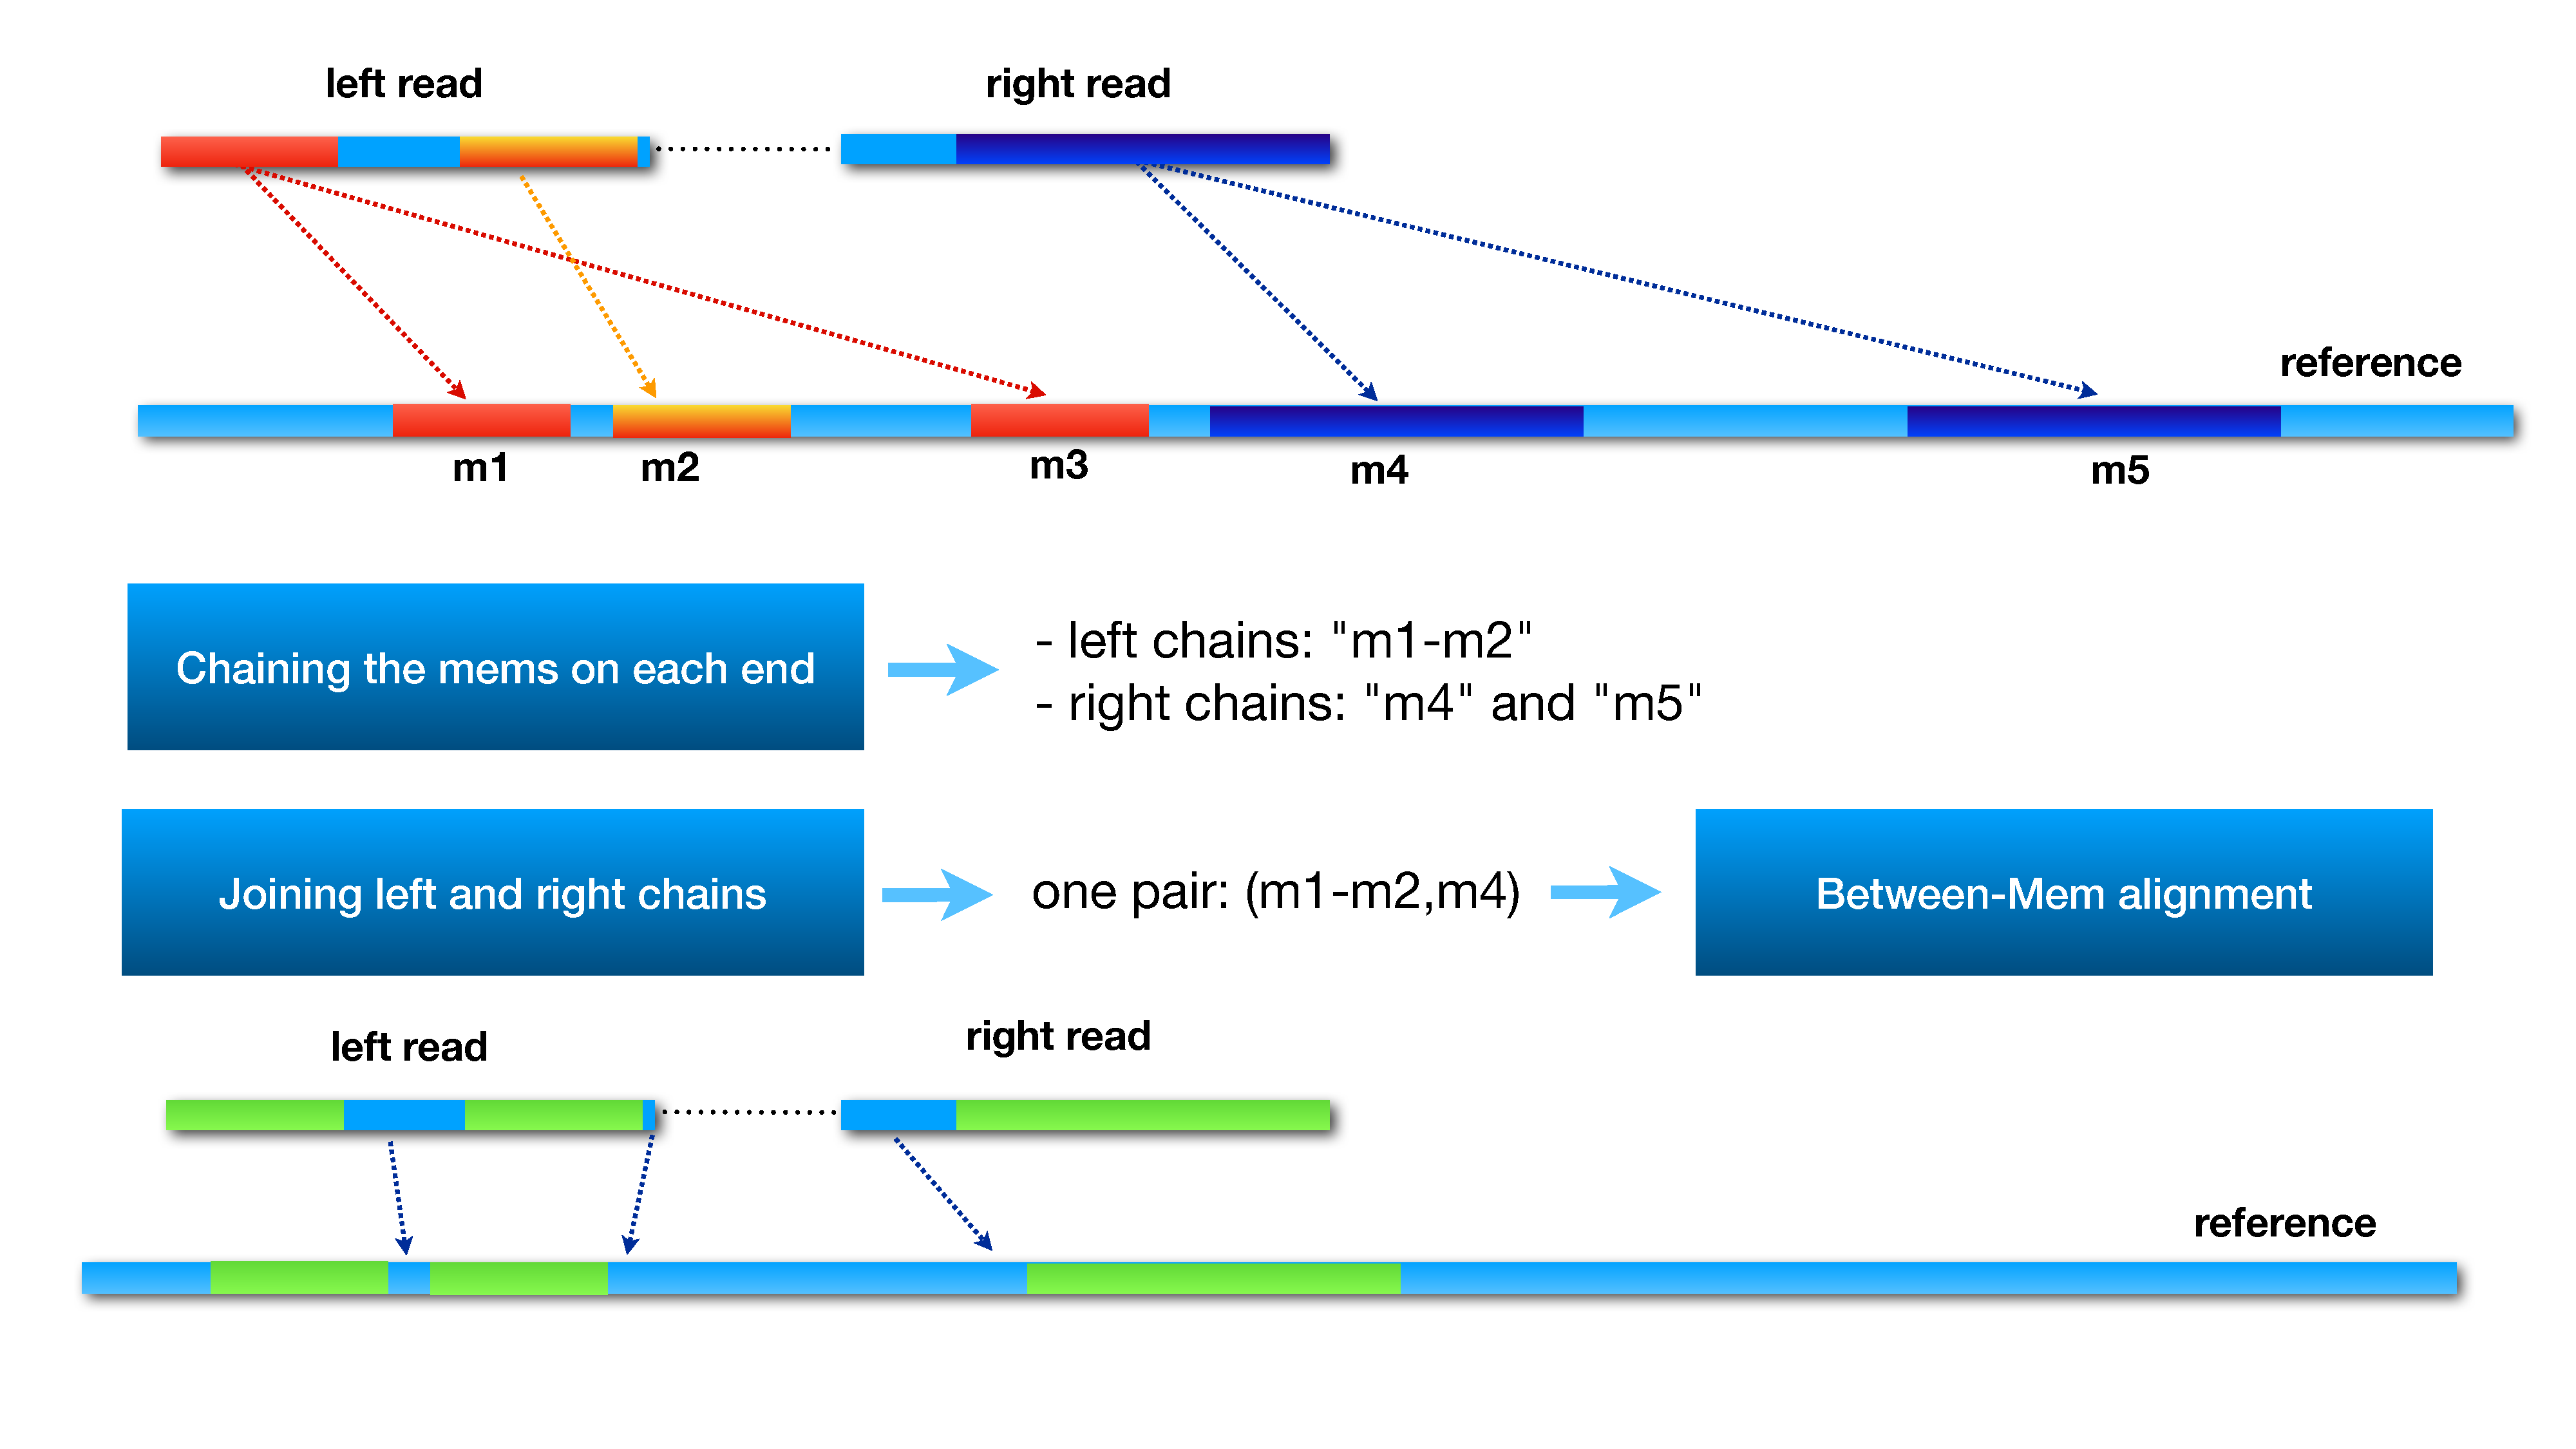
\includegraphics[width=0.95\columnwidth, trim={0in 0in 0in 0in},clip]{Figures/puff/MainFig.pdf}
    \caption[Main steps of chaining and between-\mem alignment in the \puffaligner]
    {This figure shows the main steps of chaining and
    between-\mem alignment in the \puffaligner procedure via an
    example. In this example, m1, m2 and m3 are the projected \mems
    from the left end of the read to the reference and m4 and m5 are
    the projected \mems from the right end of the read. In the first
    step, the chaining algorithm chooses the best chain of \mems that
    provide the highest coverage score for each end of the read, that
    is the m1-m2 chain for the left end and two single \mem chain for
    the right end. Then, the selected chains from each end are joined
    together to find the concordant pairs of chains, that is the
    (m1-m2, m4) pair for this read as m5 is too far from m1-m2. Then,
    the chain from each end will go through to the next step,
    between-\mem alignment. For the green areas (\mems) no alignment
    is recalculated as they are exact matches. Only the un-matched
    blue parts of the chains (those nucleotides not occurring within
    a \mem) are aligned using a modified version of \ksw. }
    \label{fig:mainScheme}
\end{figure}

In \puffaligner, if the distance between two \mems, $m_1$ and $m_2$,
on the read and the reference is $d_r$ and $d_t$ respectively, these
two \mems should not be chained together if $|d_r - d_t| > C$, where
$C$ is the maximum allowed gap. So, the penalization term, the
$\beta$ value in ~\citep{minimap2}, in the coverage score computation
is modified accordingly to prevent pairing of such \mems.

Also, unlike what is done in minimap2~\citep{minimap2}, rather than
considering together the \mems that are discovered on both ends of a
paired-end read, we consider the chaining and chain filtering for
each end of the read separately. This is done in order to make it
easier to enforce the orientation consistency of the individual
chains. Specifically, the chaining algorithm that is presented
in minimap2~\citep{minimap2} introduces a transition in the recursion that can
be used to switch between the \mems that are part of one read and
those that are part of the other. However, such switching makes it
difficult to enforce the orientation consistency of the chains that
are being built for each end of the read. One solution 
to this problem is to add another dimension to the dynamic programming
table, encoding if one has already switched from the \mems of one read end to
the other, and the recurrence can be modified to allow only one switch
from the one read end to the other, allowing enforcement of orientation
consistency. However, we found that, in practice, simply chaining the
read ends separately led to better performance.

Finally, we also adopt the heuristic proposed by minimap2~\citep{minimap2} when
calculating the highest scoring chains. That is, when a \mem is added
to the end of an existing chain, it is unlikely that a higher score
for a chain containing this \mem will be obtained by adding it to a
preceding chain. Thus, we consider only a small fixed number of
rounds (by default 2) of preceding chains once we have found the
first chain to which we can add the current \mem.

The chaining algorithm described above finds the best chains of \mems
shared between the read $r$ and the reference $t$ in orientation $o$.
A chain is accepted if its score is greater than a
configurable fraction, which we call the \textit{consensusFraction},
times the maximum coverage score found for the read $r$ to \emph{any}
reference. Throughout all the experiments in this manuscript the
\textit{consensusFraction} is set to $0.65$. If a chain passes the
consensus fraction threshold, we call it a \emph{valid} chain.
Additionally, rather than keeping all valid chains, we also filter
highly-suboptimal chains with respect to the highest scoring chain
\emph{per-reference}. All valid chains shared between $r$ and $t$ are sorted
by their scores, and chains having scores within $10\%$ 
of the highest scoring chain for reference $t$ are selected as
potential mappings of the read $r$ to the reference $t$. While these
filters are essential for improving the throughput of the algorithm
in finding the right alignment, they are carefully selected to have
very little effect on the sensitivity of \puffaligner. For
all the experiments in this manuscript, the same default settings of
these parameters are used if not mentioned otherwise.
%\mohsen{We can have an analysis of the effects of these filters in the supp}.

\subsection{Computing base-to-base alignments between \mems}
\label{subsec:base-to-base}
After finding the high-scoring \mem chains for each reference
sequence, a base-to-base alignment of the read to each of the
candidate reference sequences is computed. Each selected chain
implies a position on the reference sequence where the read might
exhibit a high quality alignment. Thus, we can attempt to compute an
optimal alignment of the read to the reference at this implied
position, potentially allowing a small bit of padding on each side of
the read. This approach utilizes the positional information provided
by the \mem chains. However, the starting position of the alignments
is not the only piece of information embedded in the chains. Rather
each chain of \mems consists of sub-sequences of the read (of size at
least $k$, though often longer) which match exactly to the reference. While the optimal
alignment of the read to the reference at the position being
considered is not \emph{guaranteed} to contain these exact matches as
alignments of the corresponding substrings, this is almost always the
case.

In \puffaligner, we aim to exploit the information from the long
matches to accelerate the computation of the alignments. In fact,
since only chains with relatively high coverage score are
selected, a large portion of the read sequences are typically already
matched to the positions in the reference with which they will be
matched in the final optimal alignment. For instance,
in~\cref{fig:mainScheme}, for the final chains selected on the
reference sequence, it is already known for the light blue, dark blue
and green sub-sequences on the left end of the read precisely where
they should align to the reference. Likewise this is the case for the yellow and
purple sub-sequences on the right read. The unmapped regions of the
reads are either bordered by the exact matches on both sides, 
or they occur at the either ends of the read sequence.
\puffaligner skips aligning the whole read sequence by considering
the exact matches of the \mems to be part of the alignment solution.
As a result, it is only required to compute the alignment of the
small unmapped regions, which reduces the computation burden of the
alignments.

When applying such an approach, two different types of alignment
problems are introduced, which we call bounded sub-sequence alignment
and ending sub-sequence alignment. For bounded sub-sequence alignment, we need
to \emph{globally} align some interval $i_r$ of the read to an
interval $i_t$ of the reference. If $i_r$ and $i_t$ are of different
lengths, the alignment solution will necessarily include insertions
or deletions. If $i_r$ and $i_t$ are of the same length, then the
optimal global alignment between them may or may not include indels.
For each such bounded sub-sequence alignment, we determine the
optimal alignment of $i_r$ to $i_t$ by computing a global pair-wise
alignment between the intervals, and stitching the resulting
alignment together with the exact matches that bound these regions.

Gaps at the beginning or the end of the read are symmetric cases, and so we
describe, without loss of generality, the case where there is an unaligned
interval of the read after the last \mem shared between the read and the
reference. In this case, we need to solve the ending sub-sequence alignment
problem. Here, the unaligned interval of the read consists of the substring
spanning from the last nucleotide of the terminal \mem in the chain, up through
the last nucleotide of the read. There is not a clearly-defined interval on
the reference sequence. While the left end of the relevant reference interval
is defined by the last reference nucleotide that is part of the bounding \mem,
the right end of the reference interval should be determined by actually solving
an extension or ``end-free'' alignment problem. We address this by performing
extension alignment of the unaligned interval of the read to an interval of the
reference that begins on the reference at the end of the terminal \mem, and
extends for the length of the unaligned query interval plus the length of some
problem-dependent buffer (which is determined by the maximum length difference  
between the read and reference intervals that would still admit an alignment
within the acceptable score threshold).

An example of both of these cases is displayed in~\Cref{fig:mainScheme}.
Specifically, an alignment of the read could be obtained by only solving two
smaller alignment problems; one is the ending sub-sequence alignment of the
unmapped region after the green \mem on the left read and the other is the
bounded sub-sequence alignment of region on the right read bordered by the
yellow and purple \mems.

\puffaligner uses \ksw~\citep{suzuki2018introducing, minimap2} for
computing the alignments of the gaps between the \mems and for aligning 
the ending sequences. \ksw exposes
a number of alignment modes such as global and extension alignments.
For aligning the bounded regions, \ksw alignment in the global mode
is performed, and for the gaps at the beginning or end of reads,
\puffaligner uses the extension mode to find the best possible
alignment of that region. \puffaligner, by default, uses a match
score of $2$ and mismatch penalty of $4$. For indels, \puffaligner
uses an affine gap scoring schema with gap open penalty of $5$ and
gap extension penalty of $3$. In \puffaligner, after computing the
alignment score for each read, only the alignments with a score
higher than $\tau$ times the maximum possible score for the read are
reported. The value of $\tau$ is controlled by the option
\textit{--minScoreFraction}, which is set to $0.65$ by default.

\subsection{Enhancing alignment computation}
\label{subsec:ksw_improvements}

By only aligning the read's sub-sequences that are not included in the \mems, the size of alignment problems being solved in \puffaligner are often much shorter than the length of the read. However, to further speed up alignment, we also incorporate a number of other techniques to improve the performance of the alignment calculation. We describe the most important of these below:

\begin{itemize}
    \item \textbf{Skipping alignment calculation by recognizing perfect chains and alignment caching:} It is possible to avoid the alignment computation completely in a considerable number of cases. In fact, as has been explained in previous work~\citep{selaln}, the alignment calculation step can be completely skipped if the set of exact matches for each chain covers the whole read. \puffaligner skips alignment for cases where the coverage score of chains of \mems is the length of the read, and assigns a total matched CIGAR string for that alignment. Alignment computation of a read might be also skipped if the same alignment problem has been already detected and computed for this read. For example, in the case of RNA seq data, reads often map to the same exons on different transcripts. In such cases, each alignment solution for a read is stored in a cache (a hash table) so that if the same alignment problem is detected, the solution can be directly retrieved from the cache, and no further computation is required (see~\cref{tab:skipped-alignments}).

    \begin{table}%[h!]
    \centering
    \begin{tabular}{lcccc}
        \toprule sample & Cache Hits & Perfect Chains & None Alignable & Total Skipped \\
        \midrule
        DNA-seq experimental & \num{52.8941105}\% & \num{19.008135}\% & \num{0.71}\% & \num{72.67}\% \\
        RNA-seq simulated & \num{28.6918391}\% & \num{50.8027558}\% & \num{0.97}\% & \num{80.46}\% \\
        Metagenomic simulated & \num{61.095958}\% & \num{31.3338897}\% & \num{0.0} \% & \num{92.43}\% \\
        \bottomrule
    \end{tabular}
    \caption[he percentage of skipped aligner engine calls]{The percentage of aligner engine calls skipped in the alignment calculation pipeline.}
    \label{tab:skipped-alignments}
    \end{table}

    %As noted in table (tab:skipped-alignments) up to 75 percent of alignment companions is skipped by considering the perfect chains and the alignment cache.
    \item \textbf{Early stopping of the alignment computation when a valid score cannot be achieved:} While care is taken to produce only high-scoring chains between the read and reference, it is nonetheless the case that the majority of the chains do not lead to an alignment of acceptable quality. Since the minimum acceptable alignment score is immediately known based on $\tau$ and the length of the read, the base-to-base alignment calculation can be terminated at any point where it becomes imposible for the minimum required alignment score to be obtained. This approach can be applied both during the \ksw alignment calculation, and also after the alignment calculation of each gap is completed. During this procedure, for each base at position $i$, starting from position $1$ on the read of length $n$, if the best alignment score $p$ up to the $i$-th position is $s_i$, we can calculate the maximum possible alignment score, $s_{max}$, that might be achieved starting at this location given the current alignment score by:
    \begin{equation}
        s_{max} = s_i + MS * (n - s_i),
    \end{equation}
    where $MS$ is the score assigned to each match. If $s_{max}$ is smaller than minimum required score for accepting the alignment, the alignment calculation can be immediately terminated, since it is already known that this anchor is not going to yield a valid alignment for this read.

    \item \textbf{Full-sensitivity banded alignment:} \ksw is able to perform banded 
    alignment to make alignment calculation more efficient. In this mode, the dynamic 
    programming matrix for the alignment problem is only filled out along the sub-diagonals 
    out to a certain distance $d$ away from the main diagonal. If one is guaranteed that any 
    valid alignment must have fewer than $d$ insertions or deletions, then the alignment must 
    not exit these bands of the dynamic programming matrix.  Note that alignments with 
    $> d$ indels can be represented within these bands as insertions and deletions move 
    in opposite anti-diagonal directions, but it is certainly the case that no alignment
    with $\le d$ indels can exit these bands. By calculating the maximum number of gaps 
    (insertions or deletions) allowed in each sub-alignment probem, in a way that we are 
    certain that any alignment having greater than this number of gaps must drop below 
    the acceptable threshold, we utilize the banded alignment in \ksw within each 
    sub-alignment problem without losing any sensitivity with respect to non-banded alignment.
\end{itemize}

\subsection{Joining mappings for read ends and orphan recovery}
\label{subsec:orphan_recovery}
Finally, once alignments have been computed for the individual ends
of a read, they must be paired together to produce valid alignments
for the entire fragment. At this point in the process, on each
reference sequence, there are a number of locations where the left
end of each read or the right end of each read, or both, are mapped 
to the reference. For the
purpose of determining which mappings will be reported as a valid
pair, the mappings are joined together only if they occur on opposite
strands of the reference, and if they are within a maximum allowed
fragment length. There are two different types of paired-end
alignments that can be reported by \puffaligner; concordant and
discordant. If \puffaligner is disallowed from reporting discordant
alignments, then the mapping orientation of the left and right end
should agree with the library preparation protocols of the reads.
\puffaligner first tries to find concordant mapping pairs on a
reference sequence, and if no concordant mapping is discovered and
the tool is being run in a mode where discordant mappings are
allowed, then \puffaligner reports pairs that map discordantly. Here,
discordant pairs may be pairs that do not, for example, obey the
requirement of originating from opposite strands. While this is not
expected to happen frequently, it may occur if there has been an
inversion in the sequenced genome with respect to the reference.

\paragraph{Orphan recovery: }  If there is no valid paired-end alignment for a fragment 
(either concordant or discordant, if the latter is allowed), then \puffaligner will attempt to 
perform orphan recovery. The term ``orphan'' refers to one end of paired-end read that is confidently 
aligned to some genomic position, but for which the other read end is not aligned nearby (and paired). 
To perform orphan recovery, \puffaligner examines the reference sequence downstream of the mapped read 
(or upstream if the mapped read is aligned to the reverse complement strand) and directly performs dynamic 
programming to look for a valid mapping of the unmapped read end. For this purpose, we use the ``fitting'' 
alignment functionality of edlib~\citep{edlib} to perform a simple Levenshtein distance based alignment that 
will subsequently be re-scored by \ksw. Finally, if, after attempting orphan recovery, there is still no valid 
paired-end mapping for the fragment, then orphan alignments are reported by \puffaligner (unless the 
``\conf{--noOrphans}'' flag is passed).

\subsection{Assessing \puffaligner's performance}

For measuring the performance of \puffaligner and comparing it to other aligners, we have designed a 
series of experiments using both simulated and experimental data from different sequencing assays. We compare 
\puffaligner with \bt~\citep{bowtie2}, \st~\citep{star} and \debga~\citep{debga}. \bt is a popular, sensitive 
and accurate aligner with the benefit of having very modest memory requirements. \st requires a much larger 
amount of memory, but is much faster than \bt and can also perform ``spliced alignment" against a reference 
(which \puffaligner, \bt, and \debga currently do not allow). \debga, is most-related tool to \puffaligner 
conceptually, as it is an aligner with a \ccdbg-based index that is focused on exploiting redundancy in the 
reference sequence.

We use different metrics to assess both the performance and accuracy of each method on a variety of types of 
sequencing samples. These experiments are designed to cover a variety of different use-cases for an aligner, 
spanning the gamut from situations where most alignments are expected to be unique (DNA-seq), to situations 
where each fragment is expected to align to many loci with similar quality (RNA-seq and metagenomic sequencing), 
and spanning the range of index sizes from small transcriptomes to large collections of genomes.

First, we show \puffaligner exhibits similar accuracy for aligning DNA-seq reads to \bt, but it is considerably 
faster. In the case of experimental reads, since the true origin of the read is unknown, we use measures such as 
mapping rate and concordance of alignments to compare the methods. Furthermore, we evaluate the accuracy of 
aligners by aligning simulated DNA-seq reads that include variation (single-nucleotide variants and small indels 
with respect to the reference). For aligning RNA-seq reads, we compare the impact of alignments produced by each 
aligner on downstream analysis such as abundance estimatation. Finally, we show \puffaligner is very efficient for 
aligning metagenomic samples where there is a high degree of shared sequence among the reference genomes being 
indexed. We also illustrate that using alignments produced by \puffaligner yields the highest accuracy for 
abundance estimation of metagenomic samples.

\subsection{Configurations of aligners in the experiments}

The performance of each tool is impacted by the different alignment scoring schemes they use, e.g. 
different penalties for mismatches, and indels. To enable a fair comparison, we attempted to configure 
the tools so as to minimize divergences that simply result from differences in the scoring schemes. For 
the experiments in this section, we use \bt in a near-default configuration (though ignoring quality values), 
and attempt to configure the other tools, as best as possible, to operate in a similar manner.

The \debga scoring scheme is not configurable, so we use this aligner in the default mode (unfortunately, 
the inability to disable local alignment and forcing just computation of end-to-end alignments in \debga makes 
certain comparisons particularly difficult). For \puffaligner we use a scheme as close to \bt as possible. The 
maximum possible score for a valid alignment in \bt is $0$ (in end-to-end mode) and each mismatch or gap subtracts 
from this score. \bt uses an affine gap penalty scoring scheme, where opening and extending a gap (insertion or 
deletion) have a cost of $5$ and $3$ respectively. For DNA-seq reads, we configure \st to allow as many mismatches 
as \bt and \puffaligner by setting the options ``\conf{--outFilterMismatchNoverReadLmax 0.12}'' and 
``\conf{--outFilterMismatchNmax 1000}''. Also, we use ``\conf{--alignIntronMax 1}'' in \st to perform 
non-spliced alignments while aligning genomic reads. For RNA-seq reads, \st has a set of parameters which 
we change in our result evaluations, and which are detailed below in the relevant sections.

In \bt we also use the option \conf{--gbar 1} to allow gaps anywhere on the read except within the first 
nucleotide (as the other tools have no constraints on where indels may occur). Furthermore, for consistency, 
we also run \bt with the option ``\conf{--ignore-quals}'', since the other tools do not utilize base qualities 
when computing alignment scores.

As explained in~\Cref{par:repetitivehits}, for the sake of performance, highly repeated anchors 
(more than a user-defined limit) will be discarded before the alignment phase.
This threshold is by default equal to $1000$ in \puffaligner. We set the threshold to the same 
value for \st and \debga using options \conf{--outFilterMultimapNmax 1000} and \conf{-n 1000} 
respectively. There is no such option exposed directly in \bt.

Since \puffaligner finds end-to-end alignments for the reads, we are also running other tools in end-to-end 
mode, which is the default alignment mode in \bt as well. In \st we enable this mode using the option 
\conf{--alignEndsType EndToEnd}. In the case of \debga, although the documentation suggests it is \emph{not} 
supposed to find local alignments by default, the output SAM file contains many reads with relatively long 
soft clipped ends, so if a read is not aligned end-to-end, \debga reports the local alignment for that.
We were not able to find any option to force \debga to perform end-to-end alignments for all reads, and 
so we have compared it in the configuration in which we were able to run it.

For aligning DNA-seq samples, each aligner is configured to report a single alignment, which is the primary 
alignment, for each read. \bt outputs one alignment per read by default. To replicate this in the other tools, 
we use the option \conf{--outSAMmultNmax 1} in \st, \conf{-o 1 -x 1} in \debga, and \conf{--primaryAlignment} 
in \puffaligner.

\subsection{Alignment of whole genome sequencing reads}

First, we evaluate the performance of \puffaligner with a whole genome sequencing (WGS) sample from 
the $1000$ Genomes project~\citep{10002015global}. We downloaded the \texttt{ERR013103} reads from sample 
\texttt{HG00190}, which is a low-coverage sample from a Finnish male, sequenced in Finland.
\footnote{https://www.internationalgenome.org/data-portal/sample/HG00190}. 
There are $18,297,585$ paired-end reads, each of length $108$ nucleotides in this sample. 
Using fastp~\citep{chen2018fastp}, we remove low quality ends and adapter sequences from these reads. 
After trimming, there are $15,404,412$ reads remaining in the sample. Indices for each of the tools 
are built over all DNA chromosomes of the latest release of the human genome (v33) by 
gencode\footnote{https://www.gencodegenes.org/human/release\_33.html}~\citep{frankish2019gencode}.

In this experiment, all aligners are configured report only concordant alignments, i.e., only pairs of 
alignments that are cocordant and within the ``maximum fragment length'' shall be reported. The maximum 
fragment length in all aligners is set to $1000$, using the option \conf{--alignMatesGapMax 1000} in \st, 
\conf{--maxins 1000} in \bt and \conf{-u 1000 -f 0} in \debga. The default value for the maximum fragment 
length in \puffaligner is set to 1000, the user can cofigure this value by using the flag 
\conf{--maxFragmentLength}. This concordance requirements also prevents \bt, \puffaligner, and \st from 
aligning both ends of a paired end read to the same strand.

The alignment rate, run-time memory usage and running time for all the aligners are presented 
in~\cref{Tab:dnaseq-exp}. The reason that \debga has the highest mapping rate in~\cref{Tab:dnaseq-exp} 
compared to other tools is that it is local alignments for the reads that are not alignable end-to-end 
under the scoring parameters for the other tools.
\bt and \puffaligner are both able to find end-to-end alignments for about $\sim95\%$ of the reads.
\st and \puffaligner are the fastest tools, with \st being somewhat faster than \puffaligner.
On the other hand, \puffaligner is able to align more reads than \st, while requiring less than half as 
much memory. The memory usage of \bt is the smallest, since \bt's index does not contain a hash table. 
However, this comes at the cost of having the longest running time compared to other methods.
Overall, \puffaligner benefits from the fast query of hash based indices while its run-time memory usage, 
which is mostly dominated by the size of the index, is significantly smaller than other hash based aligners.
Although \debga's index is based on the \dbgs, similar to the \pufferfish index, the particular encoding for 
it is not as space-efficient as that of \pufferfish.

\begin{table}%[h!]
    \centering
    \begin{tabular}{lccc}
        \toprule aligner & mapping-rate$(\%)$ & time (mm:ss) & memory (GB) \\
        \midrule
        %\puffaligner & \num{95.5495997} & 5:46 & \num{18.297428131}\\
        \puffaligner & \num{95.5831096} & 6:14 & \num{13.090557098}\\
        \debga & \num{99.7533823} & 10:46 & \num{41.040790558}\\
        \st& \num{93.880883} & 4:29 & \num{30.358268738}\\
        \bt& \num{95.4425394} & 16:15 & \num{3.5005874634}\\
        \bottomrule
    \end{tabular}
    \caption[The performance of different aligners with experimental DNA-seq reads]{The performance of different tools for aligning experimental DNA-seq reads. The time reports are benchmarked after warming up the system cache so that the influence of index loading time is mitigated.}
        \label{Tab:dnaseq-exp}
\end{table}

\begin{figure}
    \centering
    \scalebox{0.5}{
%    \includegraphics[width=0.4\linewidth,, trim={0in 0in 0in 0in},clip]
    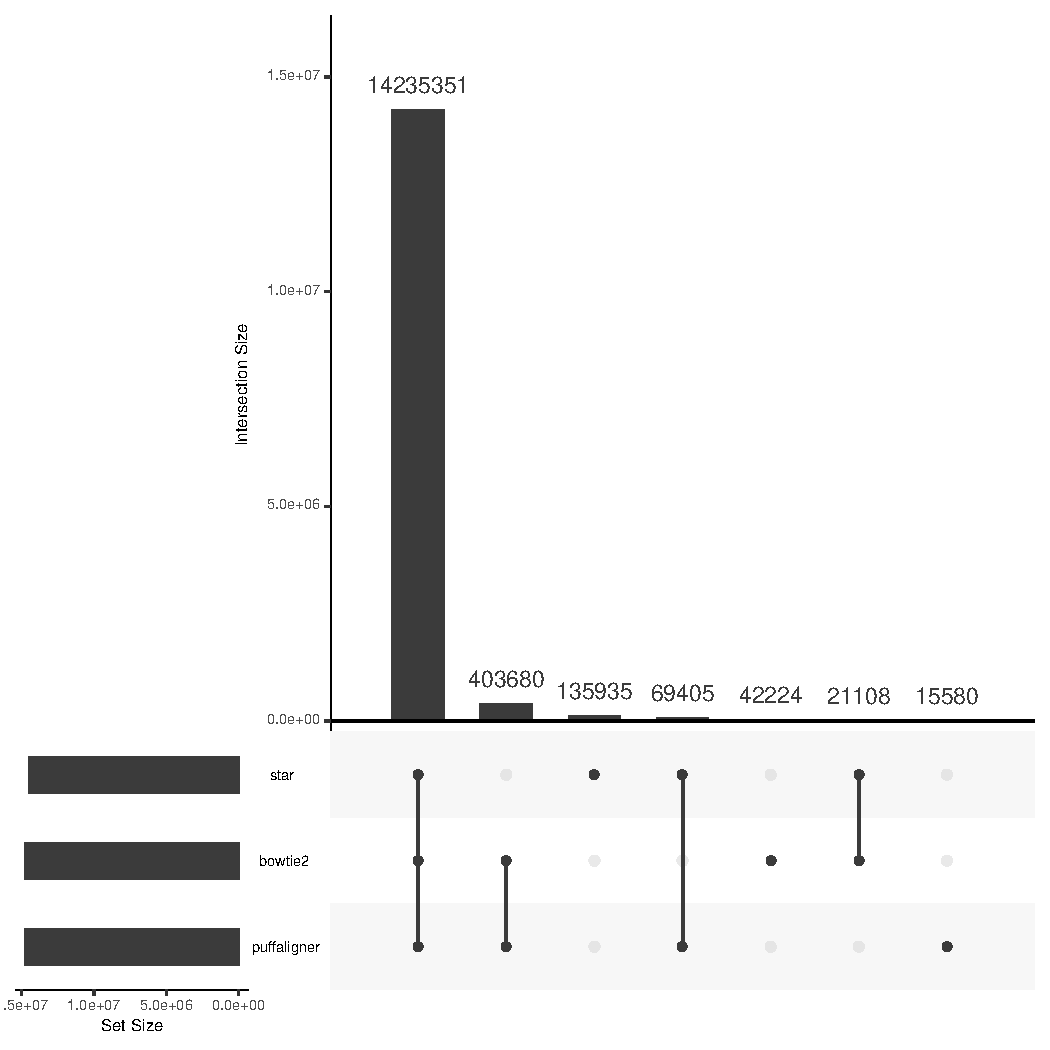
\includegraphics[trim={0in 0in 0in 0in},clip]
    {Figures/puff/ERR013103_trimmed_gencode_3tools_sparse_resubmission.pdf}}
    \caption[Upset plots for comparing the alignments - reads agreement]
    {Caomparing the alignments in terms of 
    agreement of the alignments found by different tools for each read.}
    \label{fig:upset1}
\end{figure}
\begin{figure}
    \centering
    \scalebox{0.5}{
%    \includegraphics[width=0.4\linewidth, trim={0in 0in 0in 0in},clip]
    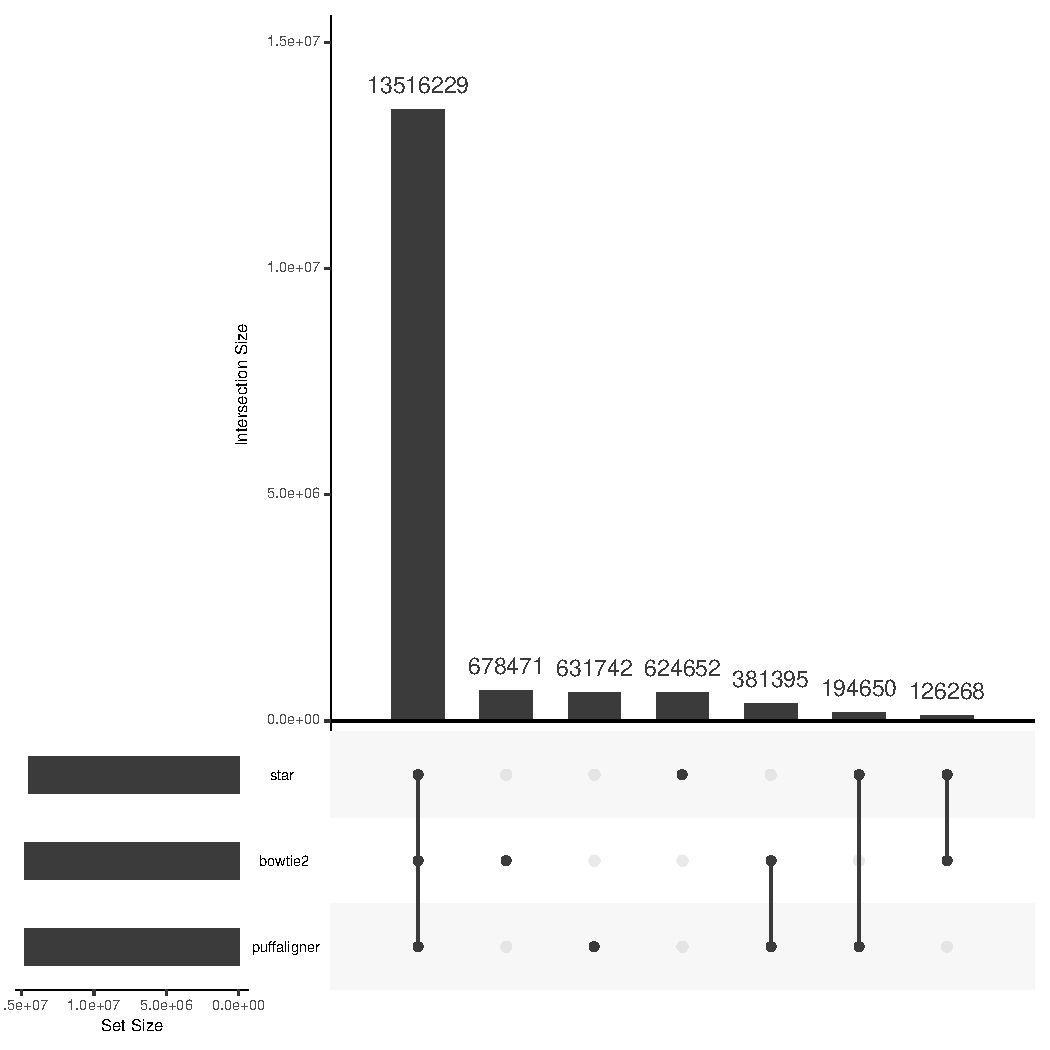
\includegraphics[trim={0in 0in 0in 0in},clip]
    {Figures/puff/ERR013103_trimmed_gencode_3tools_sparse_resubmission_location.pdf}}
    \caption[Upset plots for comparing the alignments - location agreement]
    {Caomparing the alignments in terms of 
    agreement of the alignments found by different tools based on the location of the mappings.}
    \label{fig:upset1-location}
    \label{upsetplots}
\end{figure}

To look more closely how the mappings between the tools differ, we investigate the agreement of the reads 
which are mapped by each tool and visualize the results in an upset plot in~\cref{fig:upset1} using the 
UpsetR library~\citep{conway2017upsetr}.  We are only comparing the three methods which perform end-to-end 
alignment in this plot, since outliers from the local alignments computed by \debga would otherwise dominate 
the plot. The first bar shows that the majority of the reads are mapped by all three tools.
The next largest set represents the reads which are only mapped by \bt and \puffaligner. All the other sets 
are much smaller compared to the first two sets. This fact illustrates that the highest agreement in the 
aligners is between \bt and \puffaligner. Exploring a series of individual reads from the smaller sets in 
the upset plot, suggests that some of these differences happen as a result of small differences in the scoring 
configuration, while some result from different search hueristics adopted by the different tools.
~\cref{fig:upset1-location} shows the coherence between the alignments reported by the tools by also including 
the exact location to which the reads are aligned in the reference.



\subsection{Alignment of simulated DNA-seq reads in the presence of variation}

To further investigate the accuracy of the aligners, we used simulated DNA-seq reads. One of the main 
differences between simulated reads and experimental reads is that simulated reads are often generated 
from the same reference sequences to which they are aligned, with the only differences being due to 
(simulated) sequencing error.  While (simulated) sequencing error prevents most reads from being exact 
substrings of the reference, it actually does not tend to complicate alignment too much.
On the other hand, while dealing with experimental data, the genome of the individual from which
the sample is sequenced might include different types of variations with respect to the reference 
genome to which we are aligning~\citep{srivastava2019alignment}. Therefore, it is desirable to introduce 
variations in the simulated samples, and to measure the robustness and performance of the different 
aligners in the presence of the variation. \mason~\citep{holtgrewe2010mason} is able to introduce different 
kinds of variations to the reference genome, such as SNVs, small gaps, and also structural variants (SV) 
such as large indels, inversions, translocations and duplications. We use \mason to simulate $9$ DNA-seq 
samples with different variation rates ranging from $1e-7$ to $1e-3$. Each sample includes $1M$ paired-end 
Illumina reads of $100$bp length from chromosome 21 of the human genome, ensembl release 98
\footnote{ftp://ftp.ensembl.org/pub/release-98/fasta/homo\_sapiens/dna/}. 

\begin{figure}%[H]
    \scalebox{0.8}{
    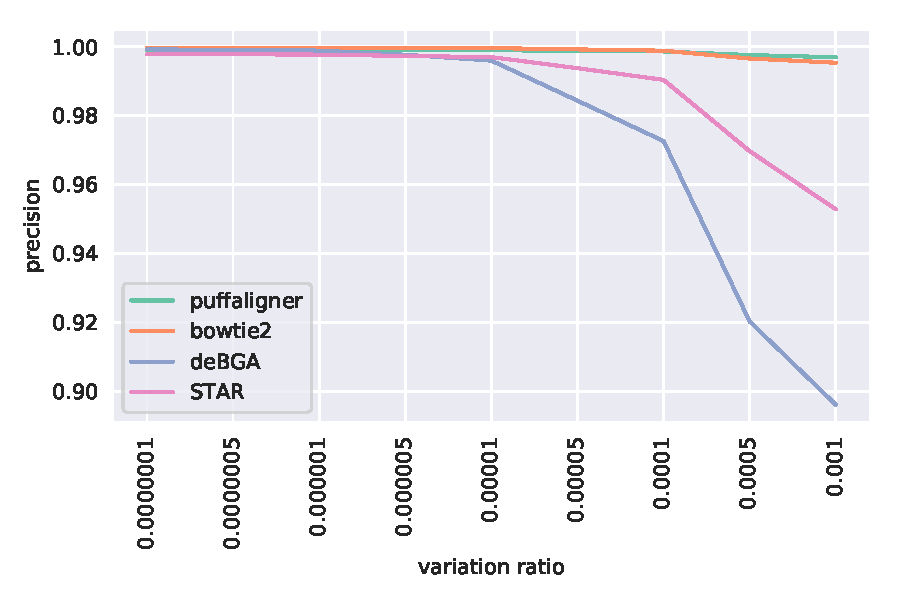
\includegraphics[width=\textwidth,type=pdf,ext=.pdf,read=.pdf]{Figures/puff/DNAseq-sim-chr21-SV-prec}}
    \caption[Accuracy of aligners in the presence of variations in the reference - precision]
    {Comparing the accuracy of aligners in the presence of different rates of variations in the reference genome
    in terms of the precision of the alignments reported by each aligner. 
    True positives (TP) are the compatible reads that are aligned to the original location, 
    and the FP set consists of both the compatible reads aligned to sub-optimal locations 
    (alignments with larger edit distance than the alignment to the original location) 
    and the non-compatible reads that are aligned with high ($>25$) edit distance.}
\end{figure}
\begin{figure}%[H]
    \scalebox{0.8}{
    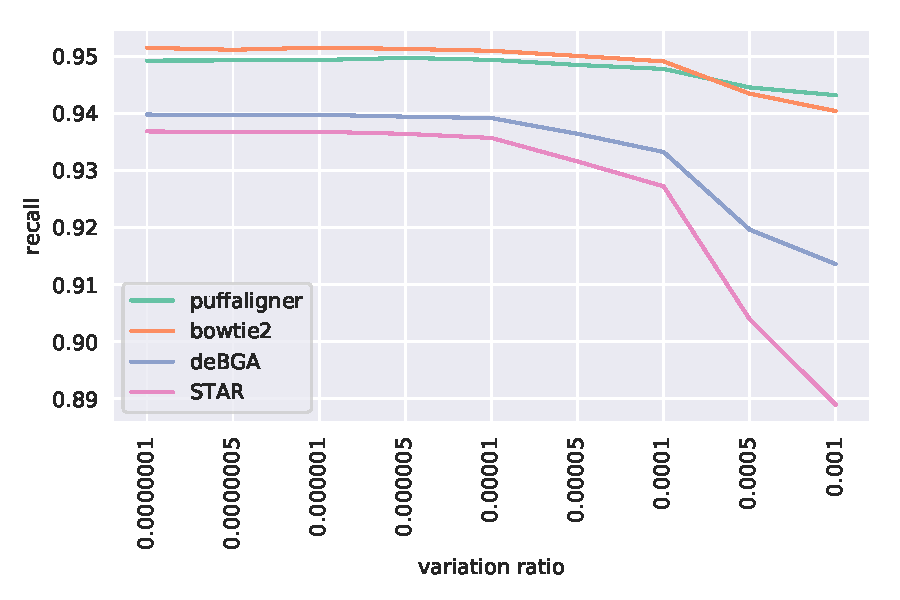
\includegraphics[width=\textwidth,type=pdf,ext=.pdf,read=.pdf]{Figures/puff/DNAseq-sim-chr21-SV-recall}}
    \caption[Accuracy of aligners in the presence of variations in the reference - recall]
    {Comparing the accuracy of aligners in the presence of different rates of variations in the reference genome
    in terms of the ratio of the alignments in the true SAM file that are recovered by each aligner. 
    The recall is the result of dividing the number of TP reads by the total number of compatible reads.}
    \label{fig:DNAseq-SV}
\end{figure}

For this analysis, we do not restrict the aligners to only report concordant alignments, since the structural variations in the samples can lead to valid discordant alignments, such as those on
the same strand or with inter-mate distances larger than the maximum fragment length. To be specific, we do not use the options which limit \bt and \puffaligner to report only concordant alignments, in addition, we use the option ``\conf{--dovetail}'' in \bt to consider dovetail pairs as concordant pairs. 

The alignments reported by \debga already include discordant pairs and also orphan mappings. Furthermore, To remove any restrictions on the fragment length in the alignments reported by \debga, we set the minimum and maximum insert size, respectively to 0 and the 50000, since setting a larger value resulted in the tool running into segmentation fault. 

To allow dovetail pairs and also larger gaps between the pairs in \st, we use the following options:\\
``\conf{--alignEndsProtrude 1000000 ConcordantPair}''\\
``\conf{--alignMatesGapMax 1000000}''\\
By default there is not a specific option in \st for allowing orphan alignment of paired end reads. Instead, we can increase the number of allowed mismatches to be as large as one end of the read by using the following options:\\
``\conf{--outFilterMismatchNoverReadLmax 0.5}''\\
``\conf{--outFilterMismatchNoverLmax 0.99}''\\
``\conf{--outFilterScoreMinOverLread 0}''\\
``\conf{--outFilterMatchNminOverLread 0}''

For each sample, \mason produces a SAM file which includes the alignment of the simulated reads to the original, non-variant version of the reference --- the version which was used for building the aligner’s indices in this experiment. Based on the alignments reported in the truth file, some reads did not have a valid alignment to the original reference. This was the result of a high rate of variations at some sequencing sites. We called the set of reads that, according to the truth SAM file, were aligned to the original reference as compatible reads.

We compared the performance of aligners based upon how well they are able to align the compatible reads. We computed the precision and recall of the alignments reported for these reads as follows. True positives are considered the reads that are mapped by the aligner to the same location stated by the truth file. Then, recall is computed by dividing the number of true positives by the number of all compatible reads. Furthermore, we considered an alignment as a false positive in two different cases. First, an alignment was considered discordant if the reported alignment had a large edit distance (larger than 25) for the non-compatible reads. Second, in the case that an aligner reported an alignment to a location other than the one in the truth file, it was considered as a false positive if the edit distance of the reported alignment is greater than the edit distance of the true alignment. Having defined the set of TP and FP for the alignments, and also having considered the set of all compatible reads as the set we are trying to recover, we computed precision and recall for the set of alignments reported by each aligner.

~\Cref{fig:DNAseq-SV} shows the precision and recall of the aligners for different samples. 
According to~\cref{fig:DNAseq-SV}, for lower variation ratios up until $10e-5$, most of the tools are 
able to make accurate alignment calls with a high specificity. As the variation ratio introduced in the 
sample is increased, all the tools start to have lower precision and recall.
\debga and \st perform worse in higher variation samples, as they fail to recover the true alignment for more 
reads, while \bt and \puffaligner are able to align most of the reads to their true 
location on the original reference.

These results show that \puffaligner' accuracy is stable in the face of variation which makes the tool 
suitable for datasets that are known to have substantial variation, such as when aligning reads to 
microbial genomes where the specific sequenced strain may not be represented in the reference set.

\subsection{Quantification of transcript abundance from RNA-seq reads}

Mapping sequencing reads to target transcriptomes is the initial step in many pipelines for reference-based 
transcript abundance estimation. While lightweight mapping approaches~\citep{kallisto,salmon} greatly speed-up 
abundance estimation by, in part, eliding the computation of full alignment between reads and transcripts, 
there is evidence that alignments still yield the most accurate abundance estimates by providing increased 
sensitivity and avoiding spurious mappings~\citep{selaln,revisit,srivastava2019alignment}. Thus, the continued 
development of efficient methods for producing accurate transcriptome alignments of RNA-seq reads remains a 
topic of interest. In this section, we compare the effect of alignments produced by each tool on the accuracy 
of RNA-seq abundance estimation.  

We generated \num{9968245} paired-end RNA-seq reads using the polyester~\citep{polyester} read simulator. 
The reads are generated by the \conf{simulate experiment countmat} module in polyester.
The input count matrix is calculated based on the estimates from the \bt-\salmon pipeline on the sample 
\texttt{SRR1085674} (where reads are first aligned with \bt and then the alignments are quantified using 
\salmon). This sample is a collection of paired-end RNA-seq reads sequenced from human transcriptome using 
an Illumina HiSeq~\citep{lonsdale2013genotype}.
The human transcriptome from gencode release (33) is used to build all the aligners' indices. Also, for 
building \st's index in the genome mode, the human genome and the comprehensive gene annotation 
(main annotation file) is obtained from the same release of gencode.

\begin{table}
    \centering
    \begin{tabular}{lcccc}
        \toprule aligner & spearman & MARD & time (mm:ss) & memory (GB) \\
        \midrule
        \puffaligner & \num{0.920247842672} &  \num{0.0524302645945} & 1:17 & \num{2.5428848267}\\
        \debga & N/A & N/A & 5:19 & \num{9.9649429321}\\
        \st - transcriptome & \num{0.920269439222} & \num{0.052751264979} & 1:57 & \num{8.7343559265}\\
        \st - genome & \num{0.900578269027} & \num{0.0641767676706} & 3:30 & \num{32.573215485}\\
        \bt& \num{0.919895559666} & \num{0.0526921568832} & 32:59 & \num{1.1455192566}\\
        \bottomrule
    \end{tabular}
    \caption[Abundance estimation of simulated RNA-seq reads]{Abundance estimation of simulated RNA-seq reads, computed by \salmon, using different tools' alignment outputs. The time and memory are only for the alignment step of each tool and the time for abundance estimation by \salmon is not considered.}
    \label{Tab:rnaseq-quant}
\end{table}

As the reads in this experiment are RNA-seq reads sequenced from the human transcriptome, it is important 
to account for multi-mapping, as often, a read might map to multiple transcripts which share the same exon 
or exon junction.
This property makes the direct evaluation of performance at the level of alignments difficult.
Therefore, a typical approach in evaluating the accuracy of the transcriptomic alignments is to assess the 
accuracy of downstream analysis such as abundance estimations by computing the correlation and relative 
differences of the estimates with the true abundance of the transcripts.
To compare the accuracy of each tool we give the alignments produced by each aligner, which are in the SAM 
format, as input to \salmon to estimate the transcript expressions.

\puffaligner, by default, outputs up to 200 alignments with an alignment score greater than $0.65$ times the 
best alignment score, i.e., the alignment for the read in the case that all bases are perfectly matched to the 
reference.
To enable the multi-mapping to take into account the characteristics of alignment to the transcriptome,
\bt is run with the option \conf{-k 200} which lets the tool output up to $200$ alignments per read. The 
value of $200$ is adopted from the suggested parameters for running RSEM~\citep{rsem} with \bt alignments. 
We note that running \bt with this option makes the tool considerably slower than the default mode, as many 
more alignments will be computed and output to the SAM file under this configuration.
For both \bt and \puffaligner, and also for \st by default, orphan and discordant mappings are not allowed.

We ran \st with the \conf{`ENCODE`} options, which are recommended in the \st manual for RNA-seq reads.
\st is also run in two different modes, one is by building the \st index on human genome, while it is also 
provided a GTF file for gene annotation. In this mode, \st performs spliced alignment to the genome, then 
projects the alignments onto transcriptomic coordinates. The other mode is building the \st index on the 
human transcriptome directly, which allows \st to align the RNA-seq reads directly to the transcripts in an 
unspliced manner. We chose to run \st in the transcriptomic mode as well, since we find that it yields higher 
accuracy, though this increases the running time of \st.

The \debga index is built on the transcriptome, as are the \bt and \puffaligner indices, since these tools 
do not support spliced read alignment. \debga is run in the with options \conf{-o 200 -x 200}, which nominally 
has the same effect as \conf{-k 200} in \bt, according to the documentation of \debga.

Accuracy of abundance estimation by \salmon, when provided the SAM output generated by each aligner, is 
displayed in~\cref{Tab:rnaseq-quant}. The timing and memory benchmarks provided in this table is only for the 
alignment step. Alignments produced by \puffaligner, \bt and \st in the transcriptomic mode produce the best 
abundance estimates. \debga's output alignments are not suitable for any abundance estimation as many reads 
are aligned only to the same strand which are later filtered during the abundance estimation by \salmon, so 
we could not provide a meaningful correlations for abundance estimation using \debga's alignments.
Aligning the reads by \st to genome and then projecting to transcriptomic coordinates does not generate as 
high correlation as directly aligning the reads to the transcriptome by \st.  However, we note that, as 
described by~\citet{srivastava2019alignment}, there are numerous reasons to consider alignment to the 
entire genome that are not necessarily reflected in simulated experiments.
While the memory usage by \puffaligner is only 2 fold larger than memory used by \bt, it computes the 
alignments much more quickly. 

According to the results in~\cref{Tab:rnaseq-quant} \puffaligner is the fastest aligner in these benchmarks, 
and the accuracy as high as \bt and \st for aligning RNA-seq reads.  Here, \puffaligner leads to the most 
accurate abundance estimates, while being $30$ times faster than \bt. Moreover, The memory usage is much 
less than other fast aligners such as \st.

\subsection{Alignment to a collection of microorganisms --- simulated short reads}

To demonstrate the performance and accuracy of \puffaligner for metagenomic samples, we designed two different 
experiments. One main property of metagenomic samples is the high similarity of the reference sequences against 
which one typically aligns, where a pair (or more) of references may be more than $90\%$ identical.
The first experiment we designed for this scenario, to specifically evaluate issues related to this challenge, 
we call the ``single strain'' experiment. Additionally, metagenomic samples also have the property of containing 
reads from a variety of genomes, some of which are not even assembled yet -- and hence unknown. This leads to 
the second experiment, which we call the ``bulk'' experiment, that compares the aligners in the presence of a 
high variety of \texttt{species} in the sample in addition to the high similarity of references.

For simplicity and uniformity, all the experiments have been run in the concordant mode for both \puffaligner 
and \bt (both of which support such an option), disallowing orphans and discordant alignments.
All aligners are run in three different confiurations, allowing three specific maximum numbers of alignments per 
fragment; 1 (primary output with highest score, breaking ties randomly), 20, and 200.
\puffaligner and \st, as the only tools that support this option, also are run in the \emph{bestStrata} mode.
In this mode, the aligner outputs all \emph{equally-best} alignments for a read with highest score without the 
limitation on number of reported alignments. This option is inspired by the similarly-named option in 
Bowtie1~\citep{langmead2010aligning}. However, unlike Bowtie1, \puffaligner and \st only make a best-effort 
attempt to find the score of the best stratum alignments, and do not guarantee to find the best stratum 
(though the cases in which they fail to seem to be exceedingly rare). This option is especially useful in 
the metagenomic analyses, as we will report only the best-score alignments without having an arbitrary 
limitation on the number of allowed alignments. This allows proper handling of highly multi-mapping 
metagenomic reads. In other words, using this option, one can achieve a high sensitivity without the need to 
hurt specificity. The details of each experiment is explained in the following sections.

\subsection{A single-strain Experiment}

For this experiment, we download the viral database from NCBI,
and choose three similar coronavirus genomes.
This set includes one of the recently-uploaded samples from Wuhan~\citep{wu2020new,baranov2005programmed}.
We select three very similar viral genomes to simulate reads from, which are: NC\_045512.2, NC\_004718.3, 
and NC\_014470.1. There are also a lot of literature discussing the similarity in sequence and behavior for 
these three species of coronavirus~\citep{wang2020unique,zhang2020probable,tang2020origin}.
The first is the complete genome for severe acute respiratory syndrome coronavirus 2 isolate Wuhan-Hu-1
known as Covid19 with length of $29,904$ bases. NC\_004718.3 is the ID of SARS coronavirus complete genome 
(length: $29,752$) and finally, NC\_014470.1 is a Bat coronavirus BM48-31/BGR/2008 complete genome 
(length: $29,277$).

We use \mason~\citep{holtgrewe2010mason} to generate three simulated samples,
each sample contains $500,000$ reads only from one of the three viral references 
we mentioned earlier. Then, reads were aligned back to the database of viral 
sequences using each of the four aligners. The results are shown in~\cref{tab:single-alignment-accuracy} 
for the reads simulated from the covid19 strain.

As the results show, the alignments of all aligners, except for \debga, are distributed only 
across the three references of interest out of all the reference sequences in the complete viral database.
\debga reports only a few alignments to a forth virus.  In general, all of the aligners do 
a good job of reporting the correct alignment among the returned alignments for each read.
Here, we are more interested in exploring how sub-optimal alignments are computed and 
filtered under different settings when aligning to a collection of very similar genomes.
The results show that all tools have very high sensitivity even when considering only 
a single (primary) alignment per read.  As we allow more alignments to be reported, 
the sensitivity increases and quickly levels off for all the tools.  On the other hand, 
more alignments are generated and \bt, in particular, generates a considerable number 
of extra alignments as the maximum number of allowed reported alignments is increased.
However, the results do not change when allowing more than 20 alignments, 
which means no more than 20 alignments ever pass the alignment score threshold for these reads in the 
viral database for any of the tools we are testing. 
    
The results indicate that, when allowing more than one alignment to be reported for every read, \bt
tends to report a large number of sub-optimal (yet, still valid) alignments compared to other tools. 
These are alignments that are accepted within the alignment score threshold, but are to another target 
than the one from which the read truly originates. Generating these sub-optimal alignments is in no way 
wrong, but it has a non-trivial computational cost, as shown in~\cref{fig:alignment_performance}, even if 
these alignments are not used in downstream analysis. Further, the score of the best alignment for each 
read is specific to that read and not known ahead of time, meaning that this situation cannot be completely 
addressed simply by setting more stringent parameters for which alignment scores should be allowed. 
This behavior of \bt gives the other tools a computational advantage when the user only truly requires 
the set of equally-best alignments for each read.
    
Interestingly, there is one read that all tools, except for \puffaligner fail to properly align.
Inspecting this alignment reveals it is a valid alignment within the range of the acceptable scoring 
threshold, and it is unclear why it is not discovered by the other tools. Overall, the aligners tested 
perform very well here in reporting the true strain of origin without reporting too many extra alignments. 
Interestingly, despite changing the parameters to allow more alignments, \st tends to return the same set 
of alignments under all configurations in this experiment.~\Cref{fig:alignment_performance} shows 
that \puffaligner has the lowest running time, even when the number of allowed alignments per read increases.

\paragraph{BestStrata Mode}

In this small example, all tools showed good sensitivity (and 
\puffaligner and \st showed near-perfect sensitivity) even when reporting
only a single-alignment per read. This experiment is, of course, an
atypically small test for multi-mapping read. In in larger samples, with
reads deriving from more organisms and a larger database of references,
permitting more alignments usually yields non-trivial improvements in
sensitivity. To control the rate of reporting sub-optimal alignments,
\puffaligner supports the ``best strata'' option -- also available to
\st, which allows only the alignments with the best calculated score to
be reported (as a replacement for maximum allowed number of alignments).
Using this option, \puffaligner achieves full specificity and sensitivity
in this experiment~\cref{tab:single-alignment-accuracy}.
We further demonstrate the positive impact of this option on the
alignment of bulk metagenomic samples in the next section.

\begin{table}%[h!]
    \centering
    \begin{tabular}{l|l|cccc}
        \toprule
        Alignment Mode 
        &
        Tool
        &
        NC\_045512.2
        &
        NC\_004718.3
        &
        NC\_014470.1
        &
        Others
        \\
        \midrule
        \multirow{4}{*}{Primary} &
        \puffaligner & \num{500000} & \num{0} & \num{0} & \num{0} \\
        &\bt & \num{499981} & 18 & \num{0} & \num{0} \\
        &\st & \num{499999} & 0 & \num{0} & \num{0} \\
        &\debga & \num{499991} & 0 & 0 & 9 \\
        \cline{1-6}
        \multirow{4}{*}{Up to 20} &
        \puffaligner & \num{500000} & \num{134} & \num{46} & \num{0}  \\
        &\bt & \num{499999} & \num{21461} & \num{2311} & \num{0}  \\
        &\st & \num{499999} & \num{0} & \num{0} & \num{0} \\
        &\debga & \num{499991} & \num{0} & \num{0} & \num{9}  \\
        \cline{1-6}
        \multirow{4}{*}{Up to 200} &
        \puffaligner & \num{500000} & \num{134} & \num{46} & \num{0}  \\
        &\bt & \num{499999} & \num{21461} & \num{2311} & \num{0}  \\
        &\st & \num{499999} & \num{0} & \num{0} & \num{0} \\
        &\debga & \num{499991} & \num{0} & \num{0} & \num{9}  \\
        \bottomrule
        \multirow{2}{*}{Best strata} &
        \puffaligner & \num{500000} & \num{0} & \num{0} & \num{0} \\
        &\st & \num{499999} & \num{0} & \num{0} & \num{0} \\
        \bottomrule
    \end{tabular}
    \caption[Alignment distribution of reads simulated from a single reference]{Alignment 
    Distribution for 500000 simulated reads from reference sequence NC\_045512.2 (known as covid19).
    The best specificity is achieved by \puffaligner in \texttt{bestStrata} mode (as well as the primary mode).
    In this simulated sample, many alignments are not ambiguous, resulting in the good performance observed 
    when using only primary alignments. However, typically in metagenomic analysis, many equally-good 
    alignments exist, and selecting only one is equivalent to making a random choice.}
    \label{tab:single-alignment-accuracy}
\end{table}

\subsection{Experiments with a mixture of organisms}

We chose a random set of $4000$ complete bacterial genomes
downloaded from the NCBI microbial database and constructed the indices of \puffaligner, \bt, \st, and 
\debga on the selected genomes.~\Cref{sfig:construction} shows the time and memory required for constructing 
each of the indices, while the size of the final index on disk is displayed in~\cref{sfig:size}.
Overall, \puffaligner and \bt show a similar trend in time and memory requirements, while \st and \debga 
require an order of magnitude more memory. In terms of the final index size, \bt has the smallest index, 
\puffaligner has the second-smallest, and \st has the largets.

For simulating a bulk metagenomic sample, we generated a list of
simulated whole genome sequencing (WGS) reads through the following steps:
\begin{itemize}
    \item Select a real metagenomic WGS read sample
    \item Align the reads of the chosen real experiment
    to the $4000$ genomes using \bt, limiting \bt to output one alignment per read.
    \item Choose all the references with count greater than \emph{C} from the quantification results.
    This defines the read distribution profile that we will use to simulate data.
    \item For each of the expressed references, use \mason~\citep{holtgrewe2010mason}, a whole genome 
    sequence simulator, to simulate $100bp$ paired-end reads with counts proportional to the reported 
    abundance estimates so that total number of reads is greater than a specified value \emph{n}.
    In this step we ran \mason with default options.
    \item Mix and shuffle all of the simulated reads from each reference into one sample which is used as 
    the mock metagenomic sample.
\end{itemize}

We selected three Illumina WGS samples that are publicly available on NCBI.
A soil experiment with accession ID \texttt{SRR10948222}~\citep{SRR10948222}
from a project for finding sub-biocrust soil microbial communities in the Mojave Desert.
The sample has $\sim27M$ paired-end reads, containing a mixture of genomes from various genera and families.
However, less than $200k$ of the reads in the sample were aligned to the strains present in our database,
leading the selection of $98$ species from a variety of genera.
We scaled the read counts in the simulation to $\sim50M$ reads. The other two selected samples are 
\texttt{SRR11283975} and \texttt{SRR11496426}
the details of which are explained in~\cref{tab:metagenome_sample_info}.
In this section we only report the performance of the tools on the first sample.

\begin{table}\centering
    \caption[Information for samples selected for simulating mock bulk metagenomic samples]
    {Basic information for samples selected for simulating mock bulk metagenomic samples. 
    The SRR10948222 sample is collected for Finding sub-biocrust soil microbial communities in Mojave Desert, 
    California, United States. The SRR11283975 sample collected from the Jiaodong Peninsula, China to study the 
    impact of different acidification degrees on the bacterial community. The SRR11496426 sample is collected 
    from the oil site of Uzon Caldera to study the composition, genetics characteristics and structure of the 
    microbial communities.}    
    \begin{tabular}{c||cccc} 
    \toprule
    Accession
    & \# of reads
    & \parbox[c]{2cm}{\# of reads \\ aligned to 4k selected reference }
    & \# of simulated reads
    & \parbox[c]{3cm}{\# of references of origin \\ for the simulated reads \\ }  \\
    \midrule
    SRR10948222
    & 27,296,270 & 200k & 5,550,650 & 98 \\
    \midrule
    SRR11283975
    & 35.5k & 8,333 & 1,012,176 & 92 \\
    \midrule
    SRR11496426
    & 42.3k & 30,203 & 1,029,382 & 179 \\
    \bottomrule
\end{tabular}
\label{tab:metagenome_sample_info}
\end{table}

The assessment of ``accuracy'' directly from the aligned reads is not a trivial task.
Due to the high rate of multi-mapping in these simulated samples, and due to the fact that multiple references 
can produce alignments of the same quality as the ``true'' origin of the read, we calculate the accuracy by 
comparing the true and estimated abundances using a quantification tool (in this case, \salmon) rather than 
by comparing the read alignments directly.

In~\cref{tab:bulk-alignment-accuracy} the accuracy metrics are calculated
over the abundance estimations obtained using the alignments produced by 
running the aligners in the different modes specified. The list of metrics for
metagenomic expression evaluations have been chosen to be similar to previous
work such as in \br~\citep{lu2017bracken} and Karp~\citep{reppell2018using}.

The metrics selected are \emph{Spearman Correlation}, \emph{Mean Absolute
Relative Difference (MARD)}, \emph{Mean Absolute Error (MAE)}, and
\emph{Mean Squared Log Error (MSLE)}. Each metric measures different
characteristics of the predicted versus true abundance estimates. For example,
lower MARD indicates better distribution of the reads among the
references relative to the abundance of each reference, while MAE shows
the quality of the distribution of the reads in a more absolute way
regardless of the difference between the abundance of the references. In
this case, one misclassified read has the same impact on the MAE metric
both for a high-abundance and low-abundance reference.

\begin{table}%[h!]
    \centering
    \scalebox{0.8}{
    \begin{tabular}{l|l|p{2cm}|cccc}
        \toprule
        \parbox[c]{3cm}{Accession ID} & \parbox[c]{0.8cm}{Alignment Mode} &\parbox[c]{2cm}{Tool}
        & Spearman
        & MARD
        & MAE
        & MSLE
        \\
        \midrule
        \multirow{14}{*}{\parbox[c]{3cm}{SRR11283975\\Jiandong Peninsula}}
        &\multirow{4}{*}{Primary} &
        \parbox[c]{2cm}{\puffaligner} & 0.71 & 0.024 & \num{0.426} & \num{0.044} \\
        &&\parbox[c]{2cm}{\bt} & 0.615 & 0.04 & \num{0.64} & \num{0.071} \\
        &&\parbox[c]{2cm}{\st} & 0.727 & 0.02 & 0.406 & \num{0.039} \\
        &&\parbox[c]{2cm}{\debga} & 0.274 & 0.521 & \num{106.776} & \num{3.788} \\
        \cline{2-7}
        &\multirow{4}{*}{Up to 20} &
        \parbox[c]{2cm}{\puffaligner} & 0.942 & 0.003 & \num{0.074} & \num{0.002}  \\
        &&\parbox[c]{2cm}{\bt} & 0.909 & 0.005 & \num{0.049} & \num{0.004}  \\
        &&\parbox[c]{2cm}{\st} & 0.946 & 0.003 & 0.087 & \num{0.002} \\
        &&\parbox[c]{2cm}{\debga} & 0.277 & 0.489 & \num{101.385} & \num{3.366}  \\
        \cline{2-7}
        &\multirow{4}{*}{Up to 200} &
        \parbox[c]{2cm}{\puffaligner} & 0.979 & 0.001 & \num{0.068} & \num{0}  \\
        &&\parbox[c]{2cm}{\bt} & 0.97 & 0.002 & \num{0.039} & \num{0.001} \\
        &&\parbox[c]{2cm}{\st} & 0.951 & 0.003 & 0.086 & \num{0.001} \\
        &&\parbox[c]{2cm}{\debga} & 0.278 & 0.483 & \num{100.961} & \num{3.293}  \\
        \cline{2-7}
        &\multirow{2}{*}{Best strata} &\parbox[c]{2cm}{\puffaligner} & 0.979 & 0.001 & 0.063 & \num{0} \\
        &&\parbox[c]{2cm}{\st} & 0.951 & 0.003 & 0.086 & \num{0.001} \\
        \bottomrule
        \midrule
        \multirow{14}{*}{\parbox[c]{3cm}{SRR11496426\\Uzon Caldera}}
        &\multirow{4}{*}{Primary} &
        \parbox[c]{2cm}{\puffaligner} & 0.568 & 0.112 & \num{32.552} & \num{0.953} \\
        &&\parbox[c]{2cm}{\bt} & 0.53 & 0.14 & \num{38.062} & \num{1.101} \\
        &&\parbox[c]{2cm}{\st} & 0.559 & 0.118 & 31.823 & \num{0.825} \\
        &&\parbox[c]{2cm}{\debga} & 0.367 & 0.566 & \num{115.882} & \num{3.569} \\
        \cline{2-7}
        &\multirow{4}{*}{Up to 20} &
        \parbox[c]{2cm}{\puffaligner} & 0.789 & 0.03 & \num{7.426} & \num{0.239}  \\
        &&\parbox[c]{2cm}{\bt} & 0.74 & 0.042 & \num{10.834} & \num{0.304}  \\
        &&\parbox[c]{2cm}{\st} & 0.713 & 0.049 & 6.939 & \num{0.165} \\
        &&\parbox[c]{2cm}{\debga} & 0.368 & 0.554 & \num{109.289} & \num{3.317}  \\
        \cline{2-7}
        &\multirow{4}{*}{Up to 200} &
        \parbox[c]{2cm}{\puffaligner} & 0.865 & 0.017 & \num{5.635} & \num{0.105}  \\
        &&\parbox[c]{2cm}{\bt} & 0.879 & 0.015 & \num{7.208} & \num{0.134} \\
        &&\parbox[c]{2cm}{\st} & 0.724 & 0.045 & 6.496 & \num{0.133} \\
        &&\parbox[c]{2cm}{\debga} & 0.369 & 0.549 & \num{108.986} & \num{3.273}  \\
        \cline{2-7}
        &\multirow{2}{*}{Best strata} &\parbox[c]{2cm}{\puffaligner} & 0.85 & 0.019 & 5.571 & \num{0.092} \\
        &&\parbox[c]{2cm}{\st} & 0.723 & 0.046 & 6.544 & \num{0.134} \\
        \bottomrule
        \midrule
        \multirow{14}{*}{\parbox[c]{3cm}{SRR10948222\\Mojave Desert}}
        &\multirow{4}{*}{Primary} &
        \parbox[c]{2cm}{\puffaligner} & 0.69 & 0.028 & \num{1.39} & \num{0.075} \\
        &&\parbox[c]{2cm}{\bt} & 0.58 & 0.053 & \num{2.91} & \num{0.153} \\
        &&\parbox[c]{2cm}{\st} & 0.727 & 0.023 & 1.493 & \num{0.048} \\
        &&\parbox[c]{2cm}{\debga} & 0.28 & 0.616 & \num{656.08} & \num{6.53} \\
        \cline{2-7}
        &\multirow{4}{*}{Up to 20} &
        \parbox[c]{2cm}{\puffaligner} & 0.9 & 0.006 & \num{0.4} & \num{0.006}  \\
        &&\parbox[c]{2cm}{\bt} & 0.85 & 0.01 & \num{0.22} & \num{0.012}  \\
        &&\parbox[c]{2cm}{\st} & 0.929 & 0.004 & 0.303 & \num{0.002} \\
        &&\parbox[c]{2cm}{\debga} & 0.28 & 0.573 & \num{637.6} & \num{5.65}  \\
        \cline{2-7}
        &\multirow{4}{*}{Up to 200} &
        \parbox[c]{2cm}{\puffaligner} & 0.97 & 0.002 & \num{0.36} & \num{0.001}  \\
        &&\parbox[c]{2cm}{\bt} & 0.99 & 0.001 & \num{0.19} & \num{0.00} \\
        &&\parbox[c]{2cm}{\st} & 0.929 & 0.004 & 0.299 & \num{0.002} \\
        &&\parbox[c]{2cm}{\debga} & 0.28 & 0.571 & \num{637.83} & \num{5.55}  \\
        \cline{2-7}
        &\multirow{2}{*}{Best strata} &\parbox[c]{2cm}{\puffaligner} & 0.97 & 0.002 & 0.36 & \num{0.001} \\
        &&\parbox[c]{2cm}{\st} & 0.929 & 0.004 & 0.3 & \num{0.002} \\
        \bottomrule
    \end{tabular}}
    \caption[Accuracy of quantification of simulated metagenomic samples using different aligners]{Accuracy of abundance estimation with \salmon using alignments reported by each aligner 
    for the mock samples simulated from the real samples with accession IDs SRR10948222, SRR11283975 and SRR11496426.
    We have run all the aligners in three main modes; allowing only one
    best alignment with ties broken randomly (Primary), up to 20
    alignments reported per read, and up to 200 alignments reported per read. \puffaligner and \st also support a mode that allows reporting all equally best
    alignments (bestStrata).}
    \label{tab:bulk-alignment-accuracy}
\end{table}

This experiment leads to three main observations. First, regardless of
the alignment mode, quantifications derived from the \debga alignments seem 
to lead to systematic underestimation of abundance.
However, \puffaligner, \st and \bt, show very similar behavior with respect to accuracy. 
\st is the best in primary mode as well as when allowing 20 alignments, closely followed by 
\puffaligner.  When allowing up to 200 alignments per read, \bt tends to yield the most accurate 
abundances, again with \puffaligner being the close runner-up. 
These results demonstrate that \puffaligner is a reliable alignment tool 
showing a stable pattern of being comparable to the best aligner under all 
the scenarios tested.  That is, the good performance of \puffaligner is robust across
a variety of different parameter settings.

Moreover, due to the nature of the metagenomic data --- the high degree of
ambiguity and multi-mapping --- we expect to see improvement in the
accuracy metrics as more alignments are reported per read, as this
leads to a higher recall. While \st's accuracy changes only slightly from
20 alignments to 200 alignments (only improving MAE) the results for
\puffaligner and \bt improve considerably when allowing more alignments per
read. However, this higher accuracy comes in the cost of alignment time
for \bt. As shown in~\cref{fig:alignment_performance}, 
\bt alignment time increases sharply when allowing more
alignments per read, while \puffaligner exhibits only small changes in alignment time 
regardless of the maximum number of alignments being reported per read. 
The difference becomes especially evident when allowing up to 200 alignments per read, 
where \puffaligner is $4$ times faster than \bt. Additionally, in experimental data, many
of the alignments reported do not necessarily have high quality, and
only appear in the output as one of the 200 alignments for the read. 
In fact, we note the similar accuracy
achieved by \puffaligner in \textit{bestStrata} mode compared to 
when we allow up to 200 alignments per read. In the other two samples
\puffaligner is the most accurate aligner in different modes for both samples.

Overall, these results along indicate that~\puffaligner is a
sensitive and fast aligner. Specifically~\puffaligner exhibits similar 
accuracy (and is sometimes more accurate) as well-known aligners like \bt and \st. 
On these data, it exhibits memory requirements close to those of the memory-frugal \bt, 
while being much faster.
\begin{figure}%[H]
    \centering
    \subfloat[] 
    {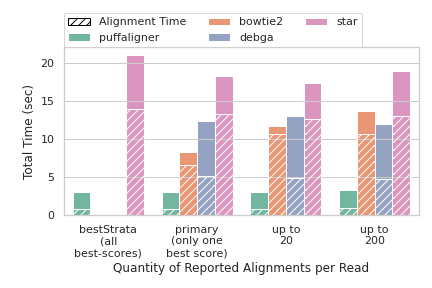
\includegraphics[width=0.8\columnwidth, type=png,ext=.png,read=.png]
    {Figures/puff/microbiome_single_time}{}}
    %{aligning a single strain sample averaged over all three samples.}}
    %\label{sfig:single_align}
    \hfill
    \subfloat[] %\centering
    {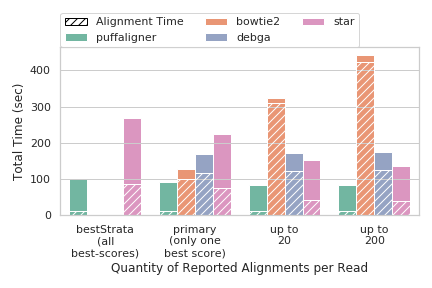
\includegraphics[width=0.8\columnwidth, type=png,ext=.png,read=.png]
    {Figures/puff/microbiome_bulk_time}{}}
    %{aligning a mock experiment simulated from bulk read sample SRR10948222.}}
    %\label{sfig:bulk_align}
    \caption[Time performance of different aligners on the microbiome
    experiments]{Time performance of different aligners on the two microbiome
    experiments. In (a), the results are averaged
    over the three alignment processes for the samples covid19, sars, and
    bat200, each having $\sim1M$ paired-end reads.
    The performance shown in (b) is for aligning reads
    in the mock sample simulated from SRR10948222 with $5M$ paired-end reads.
    As shown in the bulk experiment, the alignment for \bt
    increases when asking for more alignments per read while the other tools show a
    constant alignment time scaling over number of reads. The dashed area
    shows fraction of the time spent purely on aligning reads where the
    remaining portion is the time required for index loading. \puffaligner is 
    the fastest tool in this experiment, yet most of its time is still dedicated
    to loading the index.}
    \label{fig:alignment_performance}
    \vspace{-0.2in}
\end{figure}



\subsection{Scalability}
\begin{figure}%[h!]
    \centering
    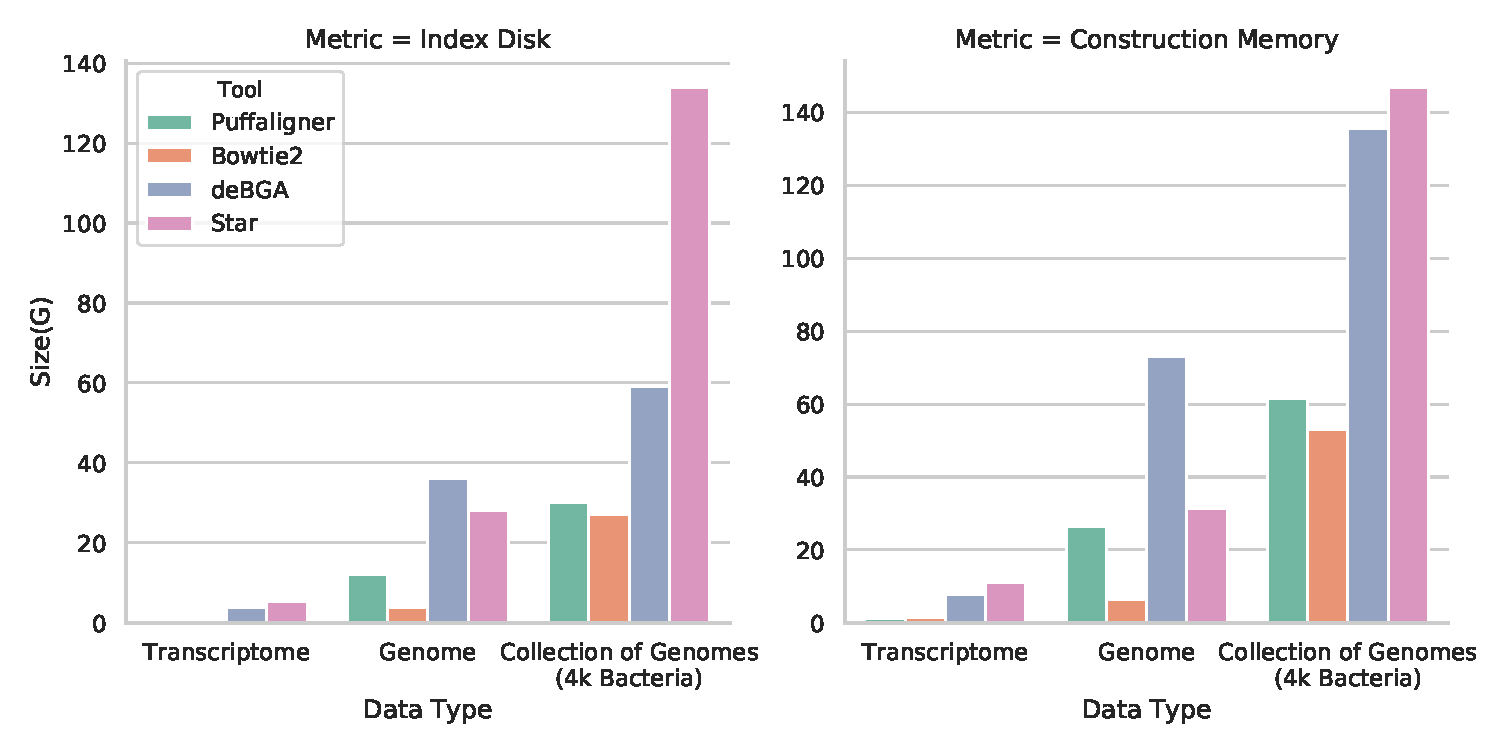
\includegraphics[width=0.8\columnwidth,type=pdf,ext=.pdf,read=.pdf]
    {Figures/puff/indexSizeScale}
    \caption[scalability of different aligners - memory]
    {Scalability of different tools over the final index disk space, construction 
    memory, for three different datasets, human transcriptome (gencode version 33), 
    human genome (GRCh38 primary assembly), and collection of genomes (4000
    random bacterial complete genomes). All tools are run with 16 threads.}
    \label{sfig:size}
\end{figure}
\begin{figure}%[h!]
    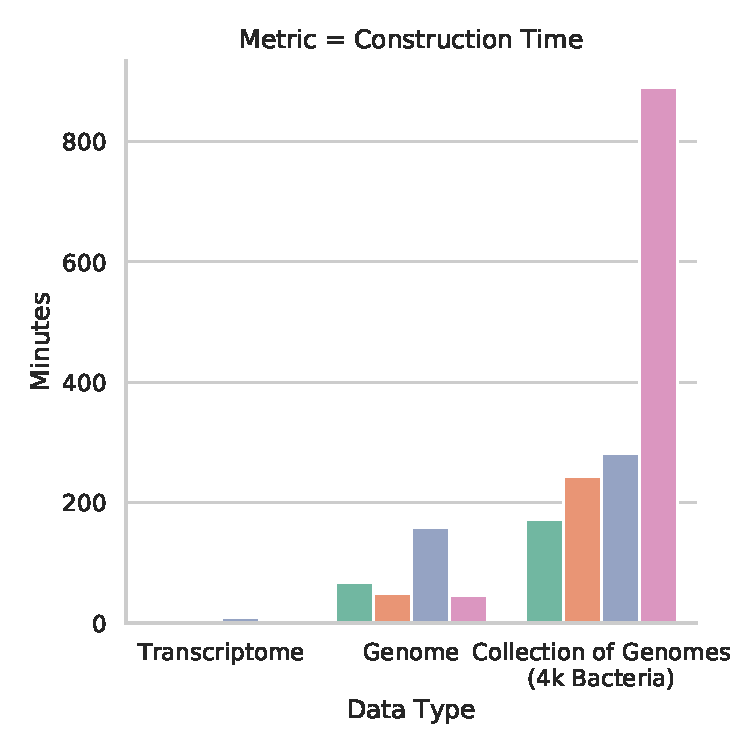
\includegraphics[width=0.8\columnwidth,type=pdf,ext=.pdf,read=.pdf]
    {Figures/puff/indexTimeScale}
    \caption[scalability of different aligners - time]
    {Scalability of different tools over the construction running time for three
    different datasets, human transcriptome (gencode version 33), human
    genome (GRCh38 primary assembly), and collection of genomes (4000
    random bacterial complete genomes). All tools are run with 16 threads.}
    \label{sfig:construction}
    \vspace{-0.2in}
\end{figure}

~\Cref{sfig:construction} and~\cref{sfig:size} represents how the construction time and
index size of each tool scales over different types of sequences. 
The trend shows the effect of database size as well as redundancy and sequence similarity on
the scalability of each of the tools. Tools such as \puffaligner and
\debga, which build a \dbg based index on the input sequence,
specifically compress similar sequences into unitigs and therefore
scale well for databases with high redundancy such as microbiomes. It is 
worth mentioning that \bt requires a switch from a $32$-bit
index to a $64$-index as the total count of the input bases
increases, which is another reason why the size is growing super-linearly.

\subsection{Discussion \& Conclusion}
\label{sec:conclusion}

In this section we introduced \puffaligner, an aligner suitable for the
contiguous alignment of short-read sequencing data. We demonstrate its
use in aligning DNA-seq reads to the genome of a single species, aligning RNA-seq reads
to the transcriptome, and aligning DNA-seq reads from metagenomic samples to a 
large collection of references. It is built on top of the \pufferfish index, which constructs
a \ccdbg using the input reference sequences. \puffaligner begins read
alignment by collecting unique maximal exact matches, querying \kmers from the
read in the \pufferfish index. The aligner then chains together the collected
uni-\mems using a dynamic programming approach, choosing the chains with the
highest coverage as potential alignment positions for the reads. Finally,
\puffaligner is able to efficiently compute alignment,
exploiting information from long matches in the chains and making use of an 
alignment cache to avoid redundant work.

We compared the accuracy and efficiency of \puffaligner against two
widely-used alignment tools, \bt and \st, that perform unspliced and
(optionally) spliced alignments of reads, respectively. We also compare
the results against \debga, an aligner that also utilizes an index built
over the compacted \dbg.

We analyze the performance of these tools on both simulated and
experimental DNA and RNA sequencing datasets. The accuracy of
\puffaligner is comparable to \bt, which exhibits very high  
alignment. \puffaligner generally performs better than \st and \debga
(though, unlike \st, none of these other tools currently support spliced read
alignment). In terms of speed and memory, \puffaligner reaches a tradeoff
between the relatively high memory usage of \st and \debga and the slower
speed of \bt. Hence, while the memory requirement of \puffaligner is more
than that of \bt, the speed gain is significant.  In the tests performed 
in this manuscript, \puffaligner is almost always the fastest tool (
with the exception being that \st is faster when aligning unspliced 
DNA-seq reads to a single human genome).

An additional advantage of the \pufferfish index utilized in \puffaligner
is that it can be built on a mixed collection of genomes, transcriptomes,
or both. This feature is already utilized in a specific pipeline for
RNA-seq quantification that makes use of a joint index over the genome 
and transcriptome~\citep{srivastava2019alignment}. The analysis shows 
that specificity of alignments in such a case can be improved by filtering 
from quantification reads that are better aligned to some genomic locus 
that is not present in the transcriptome.

Furthermore, the nature of the \pufferfish index, that explicitly
factorizes out highly-repetive sequence, coupled with the fast (and
repetition-aware) alignment procedure of \puffaligner makes it a
particularly useful for indexing and aligning to a highly similar
collection of sequences. This potentially makes it a good match 
for metagenomic analyses.

We have provided a proof of concept for such a \puffaligner-based
metagenomic analysis pipeline, and plan to build a more sophisticated 
and fully-featured metagenomic analysis framework around \puffaligner 
in the future. 
\titleformat{\chapter}
{\normalfont\large}{Appendix \thechapter:}{1em}{}
%%Appendix -- January 2015
\appendix
\renewcommand{\thechapter}{A}
\renewcommand{\chaptername}{Appendix}

\chapter{Previous Experiments}

The understanding of nonlinear processes in optical fibers is crucial towards
extending the capabilities of modern optical communication systems based on
wavelength division multiplexing (WDM), where each communication channel is
represented by a unique wavelength. One of the nonlinear processes that
limits the information carrying capacity of a WDM system is four-wave mixing
(FWM), which causes cross-talk between neighboring channels. This places a
lower limit on the wavelength separation between adjacent channels and an
upper limit on the input power in each channel. In this study, we describe
a process by which the evolution of FWM processes in an optical fiber can be
used to estimate the inhomogeneities in the fiber core material, in particular
the fluctuations in the linear refractive index of the fiber core.

\section{Overview}

Experiments measuring the evolution of FWM processes along a length of fiber
were carried out by Hart {\it et al.}\ \cite{hart1} and are described in detail in
Sec.\ 2.2. In this experiment, two input pump waves at frequencies
$\omega_1$ and $\omega_2$, interacted with each other through the third-order
nonlinearity of the fiber material to generate first-order sidebands at frequencies
$\omega_3 = 2\omega_1 - \omega_2$ and $\omega_4 = 2\omega_2 - \omega_1$.
These waves further interacted to produce second-order sidebands at
$\omega_5 = 2\omega_3 - \omega_4$ and $\omega_6 = 2\omega_4 - \omega_3$.
Higher-order sidebands were also generated. The normalized power in the
sideband at frequency $\omega_m$ was represented by $\rho_m$. The
evolution of the FWM processes was characterized by the evolution of
$\rho_m$(z) as a function of fiber length z.

In the present work, we make a quantitative comparison between these
experimental results and our numerical results based on efficient algorithms
\cite{Agrawal2} to solve the nonlinear Schr\"odinger equation (NLSE) that
governs the system. The numerical model, its underlying assumptions and
the results are described in Sec.\ 2.3. A realistic description of a
standard single mode optical fiber must take into account the random phase
perturbations a light wave undergoes while propagating through it, without
disturbing the underlying conservative properties of the system. The NLSE
needs to be suitably modified in order to incorporate the stochastic nature
of the propagation. In order to preserve the conservative properties of the
system, the stochastic terms in the NLSE must necessarily be multiplicative in
nature as an additive term acts as a source or a sink. An algorithm that
achieves this with linear, Gaussian, $\delta$-correlated noise is outlined in
Sec.\ 2.3. This algorithm preserves the unconditional stability of the
system. At the same time, care is taken to transform the stochastic NLSE from
its original Ito representation \cite{ito} to the computationally feasible Stratanovich
representation \cite{stratanovich} by compensating for the
spurious linear drift that results from integrating such stochastic
differential equations \cite{risken,werner2,drummond1,carter3}. The dominant
sources of phase noise are discussed in Sec.\ 2.4.

Conclusions on the relevance of the experiments of Hart {\it et al.}\ \cite{hart1}
and the stochastic modeling presented here are summarized in Sec.\ 2.5.

\section{Experimental and Computational Background}

In this work, we focus on tracing the evolution of the sidebands, generated
through FWM, along a length of optical fiber. The FWM spectral evolution along
50\,m of fiber for two input pump power regimes (2.1\,W and 5.5\,W) was
investigated \cite{hart1}. In the 2.1\,W case, the sideband evolution followed a damped
sinusoid along the length of the fiber. The experiments also found that the
two first-order sidebands ($\rho_3$-blueshifted and $\rho_4$-redshifted from
the two pumps) had different evolutions along the fiber (with different
spatial wavelengths). For the 5.5\,W case, the evolution of both first- and
second-order sidebands was measured. The damping in the first-order sidebands
($\rho_3$ and $\rho_4$) occured faster than in the 2.1\,W case. Experiments
probing the dependence of the sideband power on the input power (ranging from
2\,W to 17\,W) were also performed at a fixed output length of 50\,m of the fiber.
At the same fiber length, the optical spectra for input powers ranging from
2\,W to 17\,W were also recorded \cite{hart1}. The spectral envelopes were observed to fit
well to a hyperbolic secant function and the fit parameters were recorded.
Measurements with a high-resolution wavemeter showed that one of the two pumps
consisted of two very closely spaced longitudinal modes
($\Delta\nu\sim$ 0.5\,GHz) which were not resolved by the spectrometer used to
record the FWM spectra. Inclusion of this multimode nature of the pump input
in their model was found to alter the sideband dynamics dramatically and
partly explained the asymmetry between the blue-shifted and red-shifted
sidebands though it did not account for the damping in the sidebands. This
was accounted for by adding weak phase fluctuations to the waves as they
propagated along the fiber \cite{hart1}. The physical source of these phase fluctuations
was not known at that time. However, the inclusion of the phase fluctuations
into the model gave excellent qualitative and quantitative agreement with
experiment. Their model involved integration of a system of coupled ODEs
derived from the NLSE \cite{thompson1} by a process of truncation that
retained only the leading frequency components (the pumps and the first- and
second-order sidebands), a process justified by the fact that the input pump
waves are well approximated by a combination of monochromatic waves. Their
final numerical results are based on simulations using the truncated-ODE model
with Langevin noise terms representing phase fluctuations in the fiber.
Another physical source of stochasticity in their experiment was the inherent
power fluctuation in the lasers used as the input pumps. The level of
fluctuations (5-20\%) was measured and incorporated appropriately into their
model through stochastic initial conditions. This explained the evolution of
the level of observed fluctuations in the sideband trajectories although it
was found to be inadequate by itself, to account for the damping of the
trajectories. They found that all three physical characteristics mentioned
above, namely the multimode nature of the pump input, the stochastic phase
fluctuations along the length of the fiber, and the stochastic initial power
fluctuations were crucial to explaining the different features of the
experimental measurements \cite{hart1}.

\section{Stochastic NLSE Model}

In the present work, we have developed and implemented an unconditionally
stable scheme for integrating the NLSE that successfully incorporates phase
noise into the SSFM. Thus, we are now in a position to harness the high
frequency / time resolution of the SSFM together with its efficient
convergence properties. Due to these advances, we are now able to do
simulations with much higher frequency resolution (60\,MHz as compared to
300\,GHz in the ODE model). This high resolution, coupled with an appropriate
convolution scheme, enables us to compare these simulated spectra with the
composite spectra observed by the spectrometers which had a resolution of
$\sim$ 60\,GHz. This was not possible with the truncated ODE model as the
resolution of the simulated spectra in that case was $\sim$ 300\,GHz. For
exactly the same levels of phase fluctuations, and initial condition
fluctuations as used in Ref.\ \cite{hart1}, comparisons for the present NLSE
model with the experimental sideband evolution functions $\rho_i(z)$ show
excellent quantitative agreement. These results, along with the algorithms
employed, are described in detail in this section. We have identified linear
refractive index fluctuations along the fiber length to be a strong candidate
for a physical source of the stochastic phase fluctuations. A comparison
between the various possible sources is given in Sec.\ 2.4.

Under the assumption that the electric field of the light in the fiber has a
slowly varying envelope $A(z,\tau)$, and that the fiber medium has an
instantaneous nonlinear response, the system is well described by the
nonlinear Schr\"{o}dinger equation (NLSE) with a linear multiplicative
stochastic term
%A.1
\begin{equation}
{\partial U \over \partial z} + {i\beta^{(2)} \over 2T_0^2}
{\partial^2 U \over \partial\tau^2} + {\alpha U \over 2}
 + i\Gamma(z,\tau)U-i\gamma P_0 |U|^2 U = 0.
\end{equation}
$Z$ is distance along the length of the fiber,
$U(z,\tau)=A(z,\tau)/\sqrt{P_0}$ is the complex electric field envelope
$A(z,\tau)$ normalized to the absolute amplitude of the field $\sqrt{P_0}$,
$P_0$ is the total power in the fiber, $\tau$ is time normalized to a
convenient time scale $T_0(\sim 1\ ns)$ measured in a reference frame
moving with the group velocity of the pulse [$\tau=(t-z/v_g)/T_0$]. The
simulations are carried out for exactly the same physical parameters as the
experiments and simulations reported by Hart {\it et al}.\ \cite{hart1}, i.e.,
$\beta^{(2)}=55\,(ps)^2/km$, is the group velocity dispersion of the fiber at
the operating wavelength $\lambda_{0}\sim$ 632\,nm
($k_0\sim 10^7\,m^{-1}$). A loss of $\sim$ 6\,dB/km gives $\alpha$ = 0.0014\,m$^{-1}$ as the
loss in the fiber at this wavelength. The nonlinearity coefficient
$\gamma=0.019\,W^{-1}m^{-1}$ is given by
%A.2
\begin{equation}
\gamma = {\omega_{ave}n_2^I \over cA_{eff}},
\end{equation}
where $A_{eff}$ is the effective core area of the fiber,
$n_2^I$ is the Kerr coefficient for the intensity-dependent refractive index, and
$\omega_{ave}$ is the average angular frequency of the wave envelope.
$\Gamma(z,\tau)$ is a linear multiplicative phase noise field. In this study
the noise field is assumed to be $\delta$-correlated in both space and time.
The evolution of the FWM dynamics is found to be sensitive to the strength of
this noise field. It can be physically interpreted as phase noise arising due
to fluctuations in the linear refractive index of the fiber medium. A detailed
discussion of its physical origin is given in Sec.\ 2.4.

The system was simulated using the Split-Step Fourier Method (SSFM)
\cite{Agrawal2}. An algorithm for appropriately incorporating stochastic
phase fluctuations along the length of the fiber in the SSFM was developed
and is summarized below.

The NLSE is composed of linear and nonlinear terms, and can be written in operator form as
%A.3
\begin{eqnarray}
{\partial U \over \partial z} & = & (\hat{D}+\hat{S}+\hat{N})U \nonumber \\
\hat{D}& = & {-i\beta^{(2)} \over 2T_0^2}
{\partial^2 \over \partial\tau^2} - {\alpha \over 2} \nonumber \\
\hat{S} & = & i\Gamma(z,\tau) \nonumber \\
\hat{N} & = & i\gamma P_0|U|^2,
\end{eqnarray}
where $\hat{D}$, $\hat{S}$ and $\hat{N}$ are linear
(dispersive), nonlinear
and stochastic operators, respectively. It has an exact solution for
infinitesimal $\Delta z$ given by -
%A.4
\begin{equation}
U(z + \Delta z,\tau) = exp[\Delta z(\hat{D} + \hat{S} + \hat{N})]U(z,\tau) ,
\end{equation}
which can be approximated by
%A.5
\begin{equation}
U(z + \Delta z,\tau) \approx exp[\Delta z \hat{D}]exp[\Delta z \hat{S}]exp[\Delta z \hat{N}]U(z,\tau) .
\end{equation}

The execution of $exp[\Delta z \hat{N}]$ is carried out in $\tau$-space:
%A.6
\begin{equation}
B_1(z,\tau)=exp[\Delta z \hat{N}]U(z,\tau) .
\end{equation}

The execution of $exp[\Delta z \hat{S}]$ and $exp[\Delta z \hat{D}]$ is
carried out in $\omega$-space.

In particular, the stochastic phase fluctuations are introduced by modifying
the phase $\phi_j$ of each frequency component $\omega_j$ of the complex
field according to
%A.7
\begin{eqnarray}
B_2(z,\omega) & = & {\cal{F}}[B_1(z,\tau)] \nonumber \\
B_3(z,\omega_{j}) & = & exp[i \delta\phi(z,\omega_j)]B_2(z,\omega_j) ,
\end{eqnarray}
where $\cal{F}$ represents the Fourier transform operation.

This process only modifies the phase of each complex frequency component,
leaving its absolute value unchanged. Thus the algorithm conserves the total
power and the unconditional stability of the system.

The stochastic phase fluctuations $\delta\phi(z,\omega_j)$ are taken to be
$\delta$-correlated in frequency as well as spatially along the fiber length.
The Box-Muller algorithm \cite{boxmuller} was used to generate Gaussian random
deviates from computer-generated uniform random deviates $r_{1j}$ and $r_{2j}$
at each spatial step and for each frequency component $\omega_j$. The
fluctuations are given by
%A.8
\begin{equation}
\delta\phi(z,\omega_{j}) = \sqrt{-2\sigma_{\phi}^2 \Delta z ln(r_{1j})}cos(2 \pi r_{2j}) .
\end{equation}

This is followed by the execution of $exp[\Delta z \hat{D}]$, which is also
carried out in Fourier space, followed by the inverse transform
%A.9
\begin{equation}
U(z + \Delta z,\tau) = {\cal{F}}^{-1}[exp[\Delta z \hat{D}(i\omega)]B_{3}(z,\omega)] .
\end{equation}

$\hat{D}(i\omega)$ is obtained by replacing $(\partial / \partial \tau)$
by $i \omega$.

%Figure A.1
\begin{figure}
\begin{center}
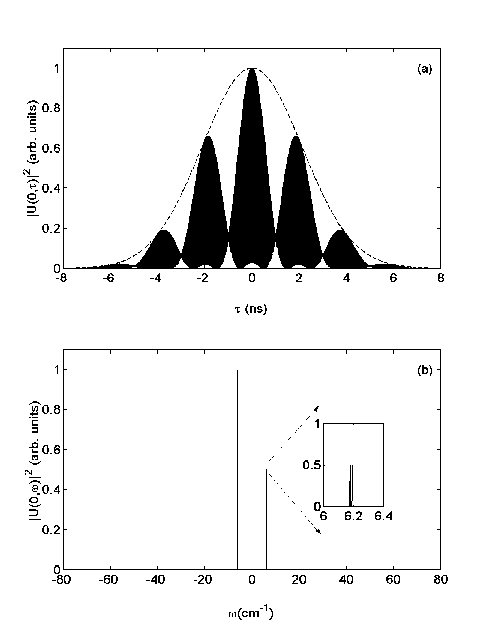
\includegraphics[width=5in]{nlsetime.pdf}
\end{center}
\renewcommand{\baselinestretch}{1}
\small\normalsize
\begin{quote}
\caption[Multimode pulse input toe NLSE]
{Multimode pulse input to the NLSE: (a) input pulse in time
domain and (b) input spectrum.}
\label{figA.1}
\end{quote}
\end{figure}
\renewcommand{\baselinestretch}{2}
\small\normalsize

The basic form of the initial complex wave envelope function is
%A.10
\begin {equation}
U(0,\tau) = exp \left( - {\tau^2 \over 2\tau_p^2} \right)
\left\{
\begin{array}{l}
exp\left( {i\Omega\tau \over 2} \right) + \\
exp\left( - {i\Omega\tau \over 2} \right)
\end{array}
\right\} ,
\end{equation}
where $\tau_p$ is the pulse width T$_p$ =5\,ns FWHM, normalized to the time scale
T$_0$, $\Omega$=366\,GHz is the frequency detuning between the two laser
sources normalized to a frequency scale $\Omega_0$ = 62.5\,MHz.  Figure A.1(a)
shows a plot of this pulse $|U(0,\tau)|^2$. The overall Gaussian envelope
has an FWHM of 5\,ns, the closely spaced dark lines are due to the 366\,GHz
($\sim$3\,ps) beating between the two input pump frequencies. The 2\,ns
modulations on the pulse are due to the 0.5\,GHz mode-structure in the
blue-shifted pump wave. Figure A.1(b) shows the input spectrum of this pulse
which consists of two highly monochromatic pump waves with a detuning of
$\Omega$=366\,GHz. The spectrum of the blue-shifted pump, upon magnification,
is seen to be composed of two very closely spaced peaks, with a separation of
$\Delta\nu$=0.5\,GHz. Hart {\it et al}.\ \cite{hart1} did not use pulsed
wave functions in their NLSE simulations as the size of the FFT required to do
so made it computationally prohibitive at that time. The size of the FFT was
chosen such that it would accommodate a time span of 16\,ns in order to go
sufficiently far into the wings on the Gaussian pulse; and a frequency span of
16\,THz in order to accommodate all the sidebands generated and prevent
spurious effects due to the reflection boundary conditions implicit in the
SSFM algorithm. These considerations dictated the size of the FFT to be
$\geq$(16 THz)$\cdot$(16 ns) = 256000. The nearest power of 2 is
2$^{18} = 262144$, which has been used throughout the present work. The
incorporation of the pulsed nature of the light was found to be necessary in
explaining the dynamics. From the perspective of the coupled amplitude
equations used by Hart {\it et al}.\ \cite{hart1}, the present model is equivalent
to a coupled-ODE model with $2^{18}$ coupled ODEs.

%Figure A.2
\begin{figure}
\begin{center}
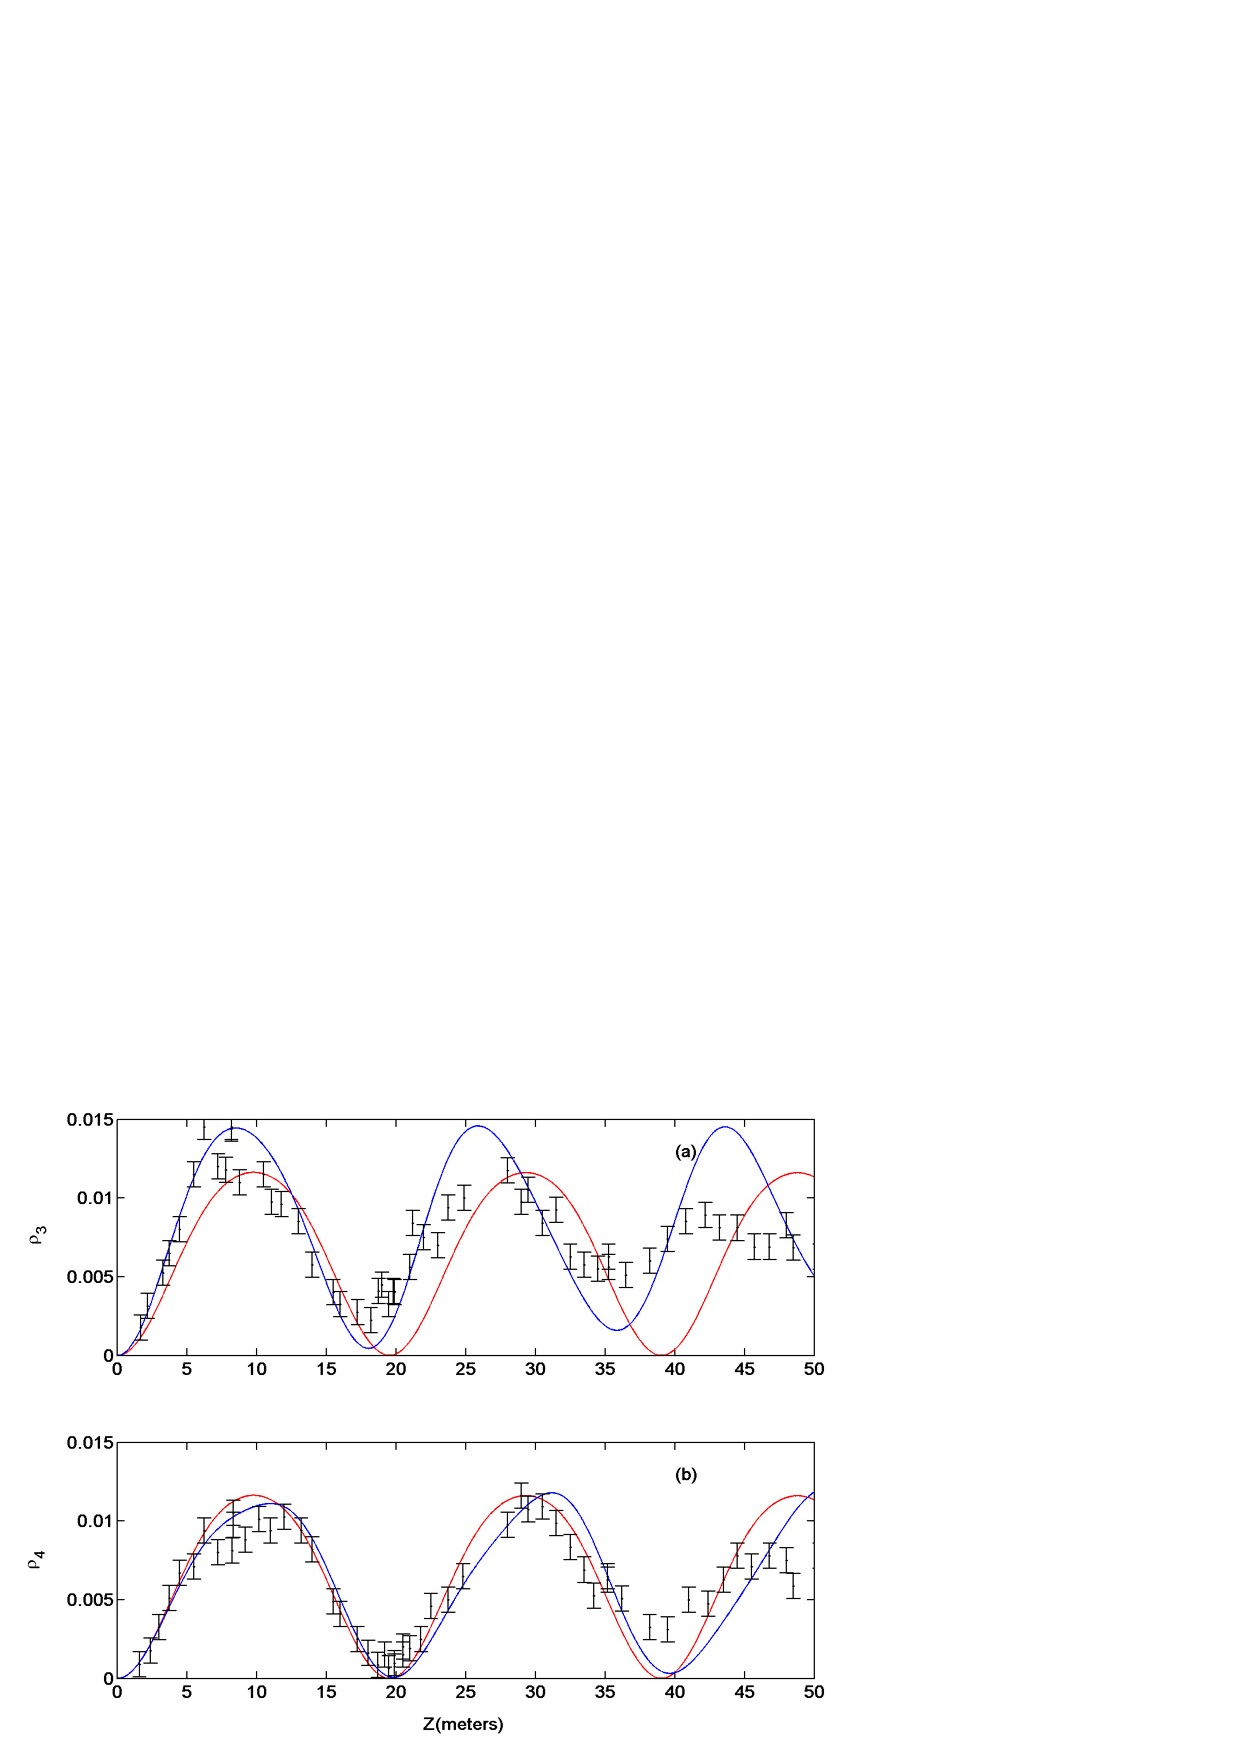
\includegraphics[width=5in]{modestruc21ornot.pdf}
\end{center}
\renewcommand{\baselinestretch}{1}
\small\normalsize
\begin{quote}
\caption[Short caption for Figure A.2.]
{Effects of inclusion of the multimode nature ($\Delta\nu = 0.5$\,GHz) of the blue-shifted input pump laser on the 1st order sideband evolution as a function of fiber length for P$_0 = 2.1$\,W. Dashed curves represent simulations without the multimode nature and solid curves represent simulations with the multimode nature. $\Omega = 366$\,GHz, $\gamma = 0.019$\,W$^{-1}$\,m$^{-1}$, and $\beta^{(2)} = 55$\,ps$^2$/km (a) power in the blue-shifted sideband, (b) power in the red-shifted sideband.}
\label{figA.2}
\end{quote}
\end{figure}
\renewcommand{\baselinestretch}{2}
\small\normalsize

%Figure A.3
\begin{figure}
\begin{center}
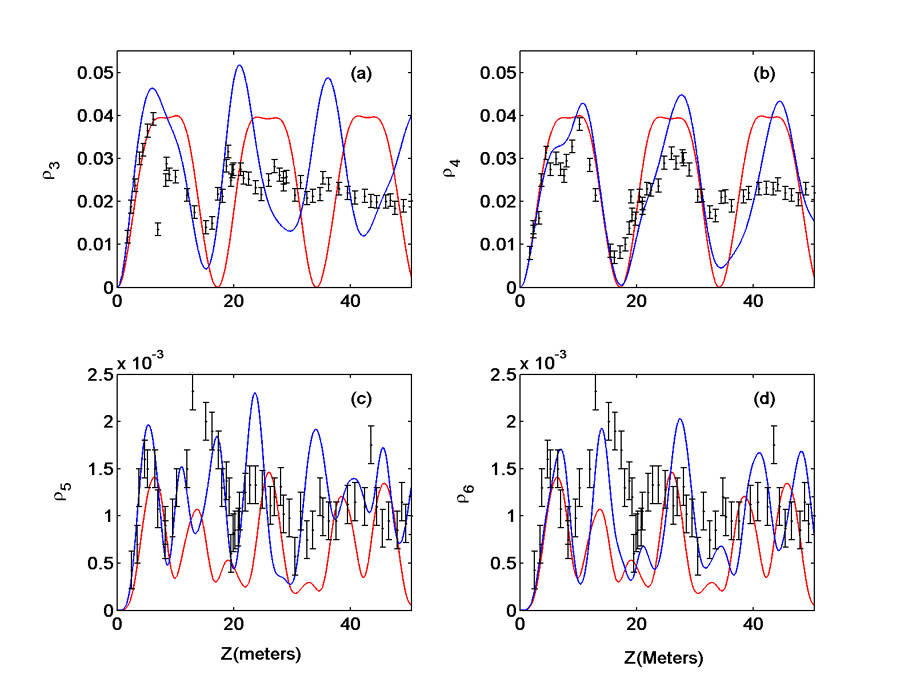
\includegraphics[width=5in]{modestruc55ornot.pdf}
\end{center}
\renewcommand{\baselinestretch}{1}
\small\normalsize
\begin{quote}
\caption[Effects of inclusion of the multimode nature]
{Effects of inclusion of the multimode nature ($\Delta\nu = 0.5$\,GHz) of the blue-shifted input pump laser on the 1st order sideband evolution as a function of fiber length for P$_0 = 5.5$\,W. Dashed curves represent simulations without the multimode nature and solid curves represent simulations with the multimode nature. $\Omega = 366$\,GHz, $\gamma = 0.019$\,W$^{-1}$\,m$^{-1}$, and $\beta^{(2)} = 55$\,ps$^2$/km (a) power in the first-order blue-shifted sideband, (b) power in the first-order red-shifted sideband, (c) power in the second-order blue-shifted sideband, (d) power in the second-order red-shifted sideband.}
\label{figA.3}
\end{quote}
\end{figure}
\renewcommand{\baselinestretch}{2}
\small\normalsize

%Figure A.4
\begin{figure}
\begin{center}
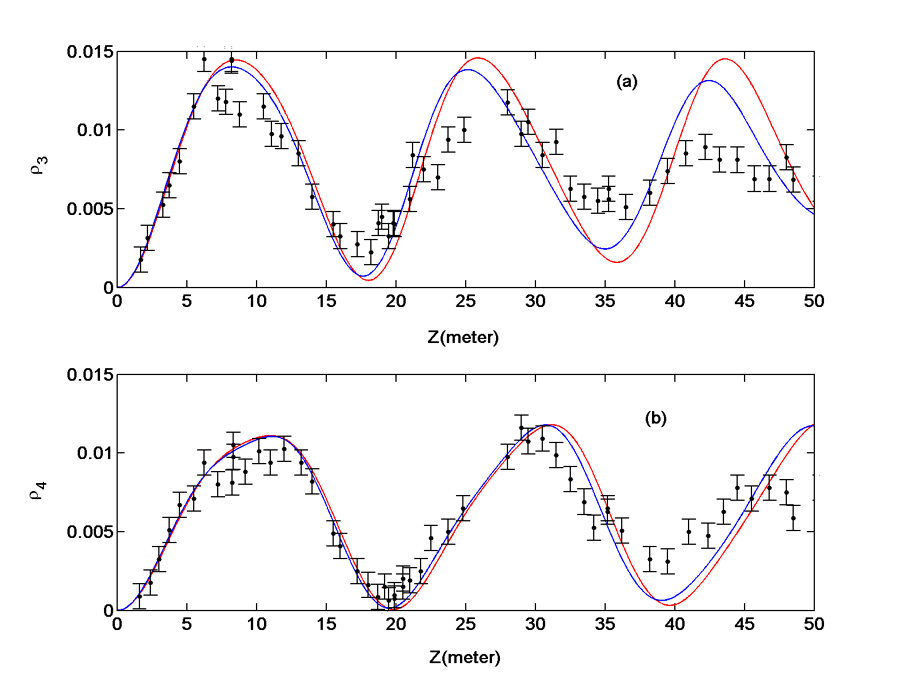
\includegraphics[width=5in]{nlsez21cwpulse.pdf}
\end{center}
\renewcommand{\baselinestretch}{1}
\small\normalsize
\begin{quote}
\caption[Effects of inclusion of the pulsed nature]
{Effects of inclusion of the pulsed nature (5\,ns FWHM) of the input pump laser light on the first-order sideband evolution as a function of fiber length for P$_0 = 2.1$\,W. Dashed curves represent cw simulations and solid curves represent pulsed simulations. $\Omega = 366$\,GHz, $\Delta\nu = 0.5$, $\gamma = 0.019$\,W$^{-1}$m$^{-1}$, and $\beta^{(2)} = 55$\,ps$^2$/,km (a) power in the blue-shifted sideband, (b) power in the red-shifted sideband.}
\label{figA.4}
\end{quote}
\end{figure}
\renewcommand{\baselinestretch}{1}
\small\normalsize

%Figure A.5
\begin{figure}
\begin{center}
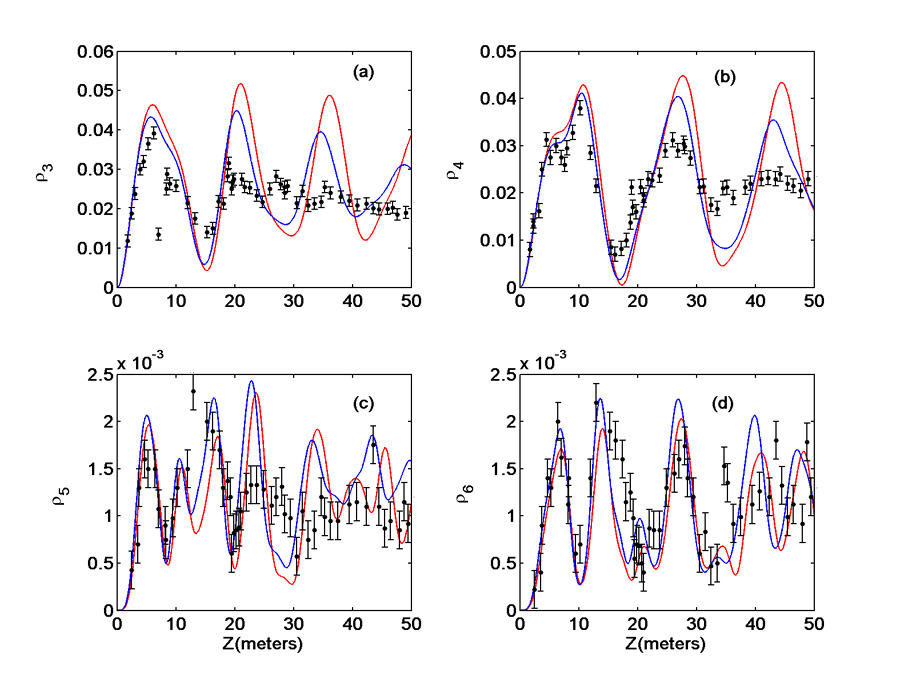
\includegraphics[width=5in]{nlsez55cwpulse.pdf}
\end{center}
\renewcommand{\baselinestretch}{1}
\small\normalsize
\begin{quote}
\caption
[Other effects of inclusion of the pulsed nature]
{Effects of inclusion of the pulsed nature (5\,ns FWHM) of the input pump laser on the first- and second-order sideband evolution as a function of fiber length for P$_0 = 5.5$\,W. Dashed curves represent cw simulations and solid curves represent pulsed simulations. $\Omega = 366$\,GHz, $\Delta\nu = 0.5$, $\gamma = 0.019$\,W$^{-1}$m$^{-1}$, and $\beta^{(2)} = 55$\,ps$^2$/,km (a) power in the first-order blue-shifted sideband, (b) power in the first-order red-shifted sideband, (c) power in the second-order blue-shifted sideband, (d) power in the second-order red-shifted sideband.}
\label{figA.5}
\end{quote}
\end{figure}
\renewcommand{\baselinestretch}{2}
\small\normalsize

Upon incorporation of the multimode nature of the blue input pump laser source
and the stochastic fluctuations in the initial power in the lasers, the
initial wave function takes the form
%A.11
\begin{equation}
U(0,\tau) = exp\left( - {\tau^2 \over 2\tau_p^2} \right)
\left\{
\begin{array}{l}
\sqrt{{1 + \delta\rho_1 \over 2}}
\left[ \begin{array}{l}
exp \left( {i(\Omega+\Delta\nu)\tau \over 2} \right) + \\
exp \left( {i(\Omega-\Delta\nu)\tau \over 2} \right)
\end{array} \right]\\
+ \sqrt{1 + \delta\rho_2} exp\left( - {i\Omega\tau \over 2} \right)
\end{array}
\right\}.
\end{equation}

\

\noindent $\Delta\nu = 0.5$\,GHz is the frequency separation between the two longitudinal
modes in the blue-shifted pump. $\delta\rho_1$ and $\delta\rho_2$ are
Gaussian random deviates (generated using the Box-Muller algorithm
\cite{boxmuller}) that represent the initial power fluctuations in each of the
pump laser sources. Their standard deviations were taken to be,
$\sigma_{\rho_1} = 0.2$, $\sigma_{\rho_2} = 0.11$ for simulations from 0\,m to
20\,m, $\sigma_{\rho_1} = 0.12$, $\sigma_{\rho_2} = 0.05$ for simulations from
20\,m to 50\,m along the length of the fiber. This is exactly the same
prescription used by Hart {\it et al}.\ \cite{hart1} in their simulations and is
dictated by their experimental measurements of the fluctuations in the pump
laser intensities.

At this point it is worth noting the effects of the inclusion of two attributes of
the input laser light, namely, the multimode nature of the blue-shifted pump, and
the pulsed nature of the input light (assumed to be cw in the simulations reported by
Hart {\it et al}.\ \cite{hart1}).

Figure A.2 shows a comparison between simulations with (solid curves) and without (dashed curves) the multimode nature for an input pump power of 2.1 Watts. The simulations with the mode structure show the asymmetry between the blue- and red-shifted sideband evolution, in particular, the difference in spatial wavelength between the two, and a non-return to zero nature of the evolution, as observed in the experimental data (black dots with error bars). These features are absent in the simulations without mode-structure. $\rho_3$ and $\rho_4$ stands for the first order blue- and red-shifted sidebands respectively.  Figure 2.3 shows the corresponding comparison for the case of 5.5 Watts of input pump power.  Here, too, the simulations incorporating the multimode nature of the blue-shifted pump (solid curves) are seen to be an improvement over those not incorporating it (dashed curves). A feature of the experimental data (black dots with errorbars) is that for the $\rho_3$ sideband, the initial part of the evolution involves a peak followed by a shoulder, while for the $\rho_4$ sideband, the initial part of the evolution involves a shoulder followed by a peak. This feature, too, is seen to occur as a result of the inclusion of the multimode nature of the blue-shifted pump.

The effect of inclusion of the pulsed nature of the input beam is seen in Fig.\ A.4 (for the 2.1 Watt case) and Fig.\ A.5 (for the 5.5 Watt case). The solid dashes represent simulations for a cw input beam and the solid curves represent those for a pulsed input beam. The incorporation of the pulsed nature clearly results in damping of the sideband trajectories which are seen to come closer to the experimental data \cite{hart1} (black dots with error bars).

Use of the FFT algorithm makes evaluation relatively fast compared to other
finite-difference schemes. The computational error is $O(\Delta z^2)$, thus
the solution converges with decreasing spatial step-size $\Delta z$.

The simulations were tested for the conservation of total power along the
fiber length (by setting the loss $\alpha$ to zero) and for the conservation
of asymmetry \cite{thompson1,hart1} given by
%A.12
\begin{equation}
C(Z) = \sum_{i=1}^{\infty}(2i-1)[\rho_{2i-1}(Z)-\rho_{2i}(Z)] .
\end{equation}

A clearer picture of the evolution of the sidebands is obtained by plotting both the
power in the sidebands and their standard deviations as a function of length along the fiber. Figures A.6(a) and A.6(b) show a comparison between simulation and experiment of the evolution
of the first-order blue-shifted ($\rho_3$) and red-shifted ($\rho_4$) sidebands,
respectively, for an input power of 2.1 W. The dashed curves represent NLSE simulations
which include the stochastic nature of the input powers of the pump lasers but exclude
the stochastic phase fluctuations added along the length of the fiber, an attribute
which is included in the simulations represented by the solid curves. The black dots
with error bars represent the experimental data. The measured sideband
power, normalized to the total power in the fiber, is periodic in length but
appears to be damping to a constant value. The measured data also show a clear
difference between the spatial wavelengths of oscillation of the blue-shifted ($\rho_3$) and red-shifted ($\rho_4$) sidebands trajectories, respectively. Both these features are captured well by both the simulations. Figures A.6(c) and A.6(d) compare experimental and simulated
measures of the evolution of the standard deviation in the sideband power
along the fiber length. It is clearly observed that simulations with phase noise
added to the light field along the length of the fiber (solid curves) are closer to the
experimental data as compared to those that exclude this feature (dashed curves). This indicates
the instrumental nature of the phase fluctuations in explaining key features of the dynamics.

%Figure A.6
\begin{figure}
\begin{center}
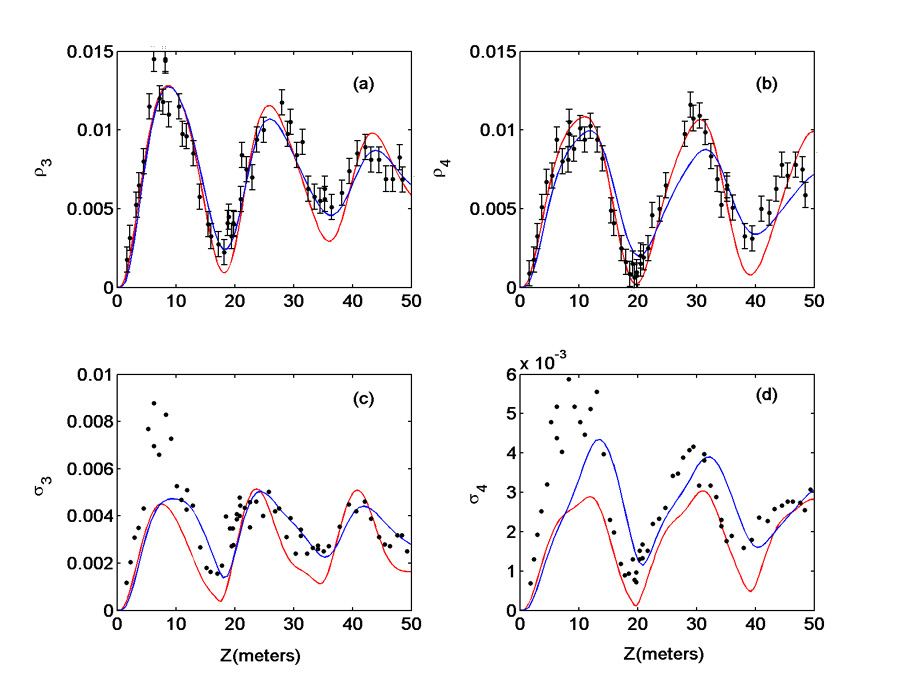
\includegraphics[width=5in]{nlsez21phaseornot.pdf}
\end{center}
\renewcommand{\baselinestretch}{1}
\small\normalsize
\begin{quote}
\caption
[Comparison between experiments measurements]
{Comparison between the experimental measurements \cite{hart1}(black), the random initial condition NLSE model excluding phase noise (dashed curves) and the stochastic phase noise NLSE model (solid curves) showing the first-order sideband evolution as a function of fiber length for P$_{0} = 2.1$\,W, $\Omega = 366$\,GHz, $\Delta\nu = 0.5$\,GHz,$\gamma = 0.019$\,W$^{-1}$m$^{-1}$, and $\beta^{(2)} = 55$ps$^2$/km: dynamical evolution of the: (a) power in the blue-shifted sideband, (b) power in the red-shifted sideband, (c) fluctuations in the blue-shifted sideband, (d) fluctuations in the red-shifted sideband.}
\label{figA.6}
\end{quote}
\end{figure}
\renewcommand{\baselinestretch}{2}
\small\normalsize

The apparent damping of the periodic sideband trajectory is seen more
dramatically in Figs.\ A.7(a) and A.7(b), which show the evolution of the
first-order sideband power along the fiber for an input power of 5.5\,W.
The two first-order sidebands evolve differently. They appear to
damp to a constant value at a faster rate than for the case with an input pump
power of 2.1\,W. Here again, NLSE simulations that incorporate phase noise along the length
of the fiber (solid curves) are much more successful in accurately capturing the dynamical features of the system than NLSE simulations that do not take this feature into account (dashed curves).  Figures A.7(c) and A.7(d) show a comparison between the simulated and measured standard deviations. Comparisons for the second-order blue-shifted ($\rho_5$) and red-shifted ($\rho_6$) sidebands, respectively, are shown in Figs.\ A.7(e) and A.7(f).


%Figure A.7
\begin{figure}
\begin{center}
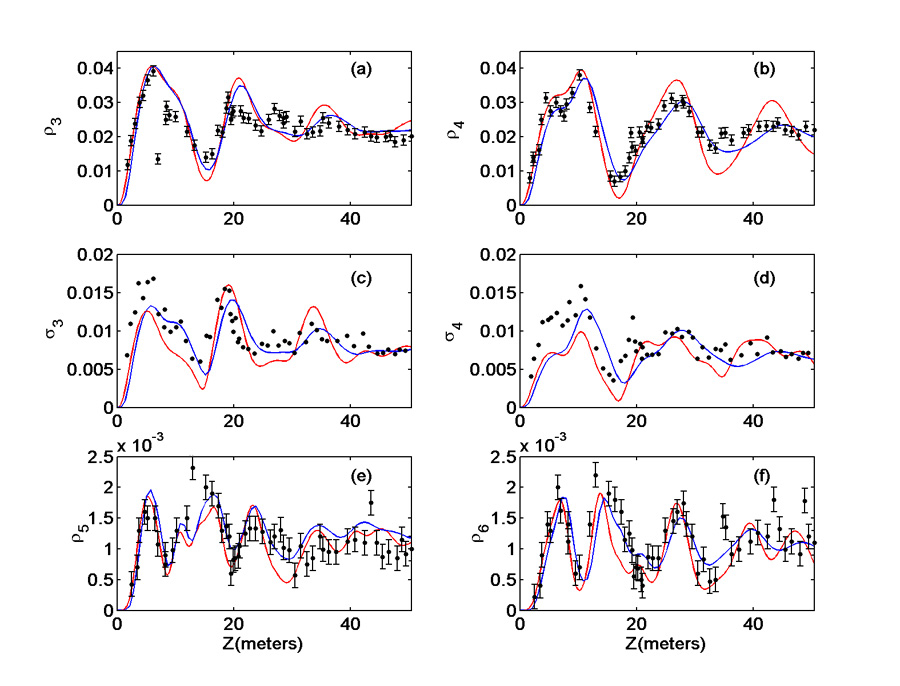
\includegraphics[width=5in]{nlsez55phaseornot.pdf}
\end{center}
\renewcommand{\baselinestretch}{1}
\small\normalsize
\begin{quote}
\caption
[This figure caption is indented and single-spaced]
{This figure caption is indented and single-spaced.  Comparison between the experimental measurements \cite{hart1} (black), the random initial condition NLSE model excluding phase noise (dashed curves) and the stochastic phase noise NLSE model (solid curves) showing the first- and second-order sideband evolution as a function of fiber length for P$_{0} = 5.5$\,W, $\Omega = 366$\,GHz, $\Delta\nu = 0.5$\,GHz, $\gamma = 0.019$\,W$^{-1}$m$^{-1}$, and $\beta^{(2)} = 55$\,ps$^2$/km: dynamical evolution of the: (a) power in the first-order blue-shifted sideband, (b) power in the first-order red-shifted sideband, (c) fluctuations in the first-order blue-shifted sideband, (d) fluctuations in the first-order red-shifted sideband, (e) power in the second-order blue-shifted sideband, (f) power in the second-order red-shifted sideband.}
\label{figA.7}
\end{quote}
\end{figure}
\renewcommand{\baselinestretch}{2}
\small\normalsize

The observed dynamical evolution of the sidebands is found to depend
sensitively on the strength of the stochastic phase fluctuations. Yet, best
agreement with the experimental results of Hart {\it et al}.\ \cite{hart1} is
achieved with exactly the same noise strength $\sigma^2_\phi$ as used in
their truncated ODE model, namely, $\sigma^2_\phi = 0.0067$\,m$^{-1}$. They
report that including phase noise in their FWM calculations resulted in a
spurious linear drift in the trajectories for the sideband power with length.
To remove this artifact of the computations, they added a linear loss to their
coupled ODEs. They set the loss coefficient $\alpha = 0.0046$\,m$^{-1}$ by
finding the value that removed this increasing slope. We have observed exactly
the same secular growth phenomenon for a wide range of the noise strength
$\sigma^2_\phi$ and have arrived at an empirical prescription for $\alpha$
namely, $\alpha\sim\sigma^2_\phi$, where $\sigma^2_\phi$ is the
variance of the added phase noise. This indicates the general nature of
dynamics resulting from the addition of stochastic, $\delta$-correlated phase
fluctuations to systems governed by nonlinear partial differential equations
\cite{risken}.

It is remarkable that the strength of the phase noise required is the same in
both the 2.1\,W and the 5.5\,W cases. Further, it is worth noting that exactly
the same noise strength was used by Hart {\it et al}.\ \cite{hart1}, the difference
being that they introduced phase noise only in the pump frequencies, whereas
we have introduced it in all the Fourier modes ($\sim2^{18}$). As a
confirmation of this result, they also performed experiments and numerical
simulations examining the sideband power dependence on the input power at a
fixed length of 50.4\,m of the same fiber. We have repeated these simulations
with the stochastic NLSE model and the results are shown in Figs.\ 2.8(a)
(blue-shifted sideband) and 2.8(b) (red-shifted sideband). The experimental
measurements of the sideband powers are represented by filled squares and the
results of numerical simulations are represented by triangles (without phase
noise) and by circles (with phase noise). The simulations are seen to follow
the general trend seen in the experiments. As the pump power is increased, the
triangles (without phase noise) start to disagree with experiment, whereas the
circles (with phase noise) are much closer to experiment. The phase noise
strength used in these simulations was exactly the same as that used in the
simulations depicted in Figs.\ A.6 and A.7. The agreement between the phase noise
simulations and the experimental data was (once again) highly sensitive to the
noise strength. Since this experiment (unlike those shown in Figs.\ A.2 - A.7)
is non-destructive, it can be used to deduce the strength of phase noise
processes in a given optical fiber. It will be shown in Sec.\ 2.4 that a
likely cause of the phase noise is fluctuation in the linear refractive index
of the fiber. The noise strength deduced from the present computational study
corresponds to a refractive index inhomogeneity of
$\langle \Delta n^{2} \rangle \sim 10^{-16}$.

%Figure A.8
\begin{figure}
\hspace{1.25in}
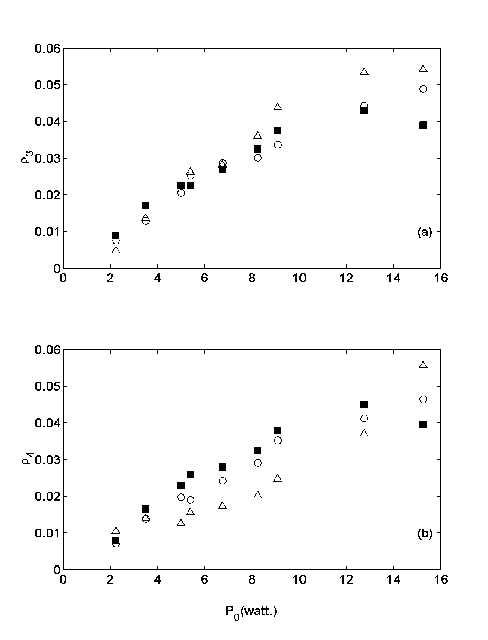
\includegraphics[width=5in]{nlsefinal.pdf}
\renewcommand{\baselinestretch}{1}
\small\normalsize
\begin{quote}
\caption
[Comparison between the experiments measurements (filled squares)]
{Comparison between the experimental measurements (filled squares), simulations without stochastic phase fluctuations (open triangles) and with stochastic phase fluctuations (open circles) of the first-order sideband power versus pump input power for L=50.39\,m, and $\Omega = 366$\,GHz: power in the (a) blue-shifted sideband and (b) red-shifted sideband.}
\label{figA.8}
\end{quote}
\end{figure}
\renewcommand{\baselinestretch}{2}
\small\normalsize

%Figure A.9
\begin{figure}
\begin{center}
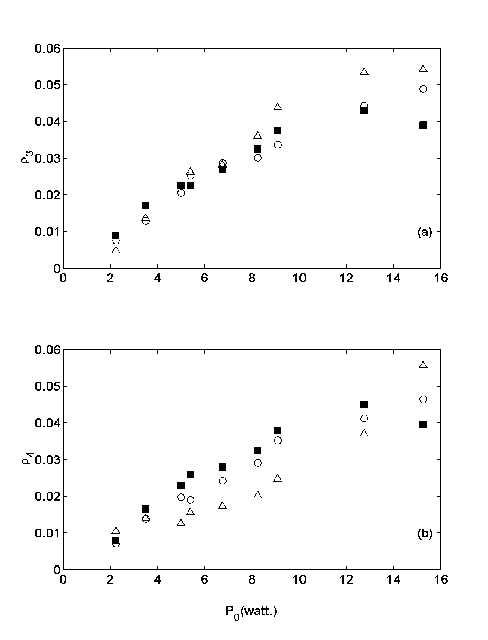
\includegraphics[width=5in]{nlsefinal.pdf}
\end{center}
\renewcommand{\baselinestretch}{1}
\small\normalsize
\begin{quote}
\caption
[Evolution of the FWM spectrum]
{Evolution of the FWM spectrum along the fiber (a) P=2.1\,W, experiment, (b) P=5.5\,W, experiment, (c) P=2.1\,W, stochastic-NLSE model, (d) P=5.5\,W, stochastic-NLSE model.}
\label{figA.9}
\end{quote}
\end{figure}
\renewcommand{\baselinestretch}{2}
\small\normalsize

Till now the comparisons between our simulations of the full NLSE and the
truncated ODE model give basically the same results, although with much better
agreement with experiment. However, the full NLSE can also provide a detailed
comparison with the experimental spectra. This was not available from the
truncated ODE model. The simulations reported in this work were carried out
with a very high frequency and time resolution in order to incorporate the
fact that the input light was not cw, but was composed of $\sim$ 5\,ns long
pulses; and that the number of sidebands generated required the frequency
spread of the FFT to be $\sim$ 16\,THz, while resolving a longitudinal
mode-structure of $\Delta\nu$ $\sim 0.5$\,GHz. The spectral resolution used was
$\sim$ 0.05\,GHz, whereas the spectrometer used to observe the spectra had a
resolution 1000 times larger ($\sim$ 50\,GHz). To account for this difference,
the simulated spectra were first convolved with a Gaussian of unit peak and
62\,GHz FWHM, before they were compared with the observed spectra.

Figures A.9(a) and A.9(b) show three-dimensional plots of the average experimental
FWM output spectrum along the length of the fiber for input pump powers of 2.1\,W and 5.5\,W,
 respectively (courtesy Hart {\it et al}.\ \cite{hart1}). The vertical
axis represents the intensity, normalized to the peak power in one of the
input pumps, plotted on a logarithmic scale. The pump frequencies are centered
on $+/-\Omega/2$ and the fiber length is increasing into the page. Figures
9(c) and 9(d) show the corresponding comparisons based on simulations using
the stochastic-NLSE model. The basic features of the spectral evolution are
captured by the simulations.

%Figure  A.10
\begin{figure}
\begin{center}
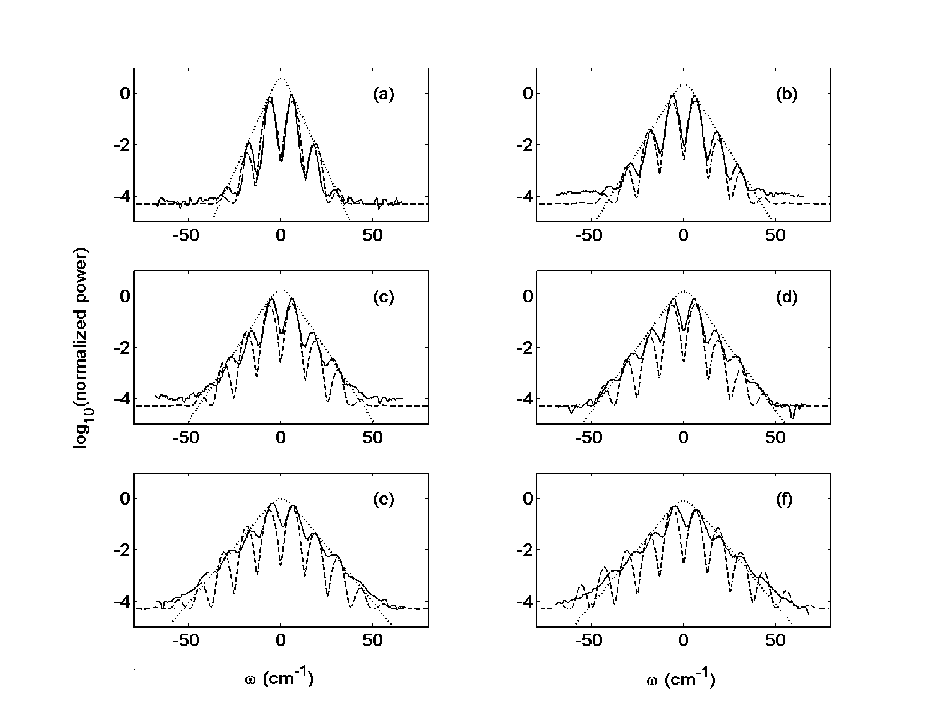
\includegraphics[width=5in]{nlsespec.eps}
\end{center}
\renewcommand{\baselinestretch}{1}
\small\normalsize
\begin{quote}
\caption
[Experimental FWM output spectrum]
{Experimental FWM output spectrum (solid line), convolved spectra from simulations of the stochastic NLSE model (dashed line), and hyperbolic secant envelope fit (dotted line) for pump input powers P$_0$ of (a) 2.1\,W, (b) 5.5\,W, (c) 6.7\,W, (d) 8.3\,W, (e) 12.7\,W, (f) 17.4\,W, fiber length L$= 50.39$\,m, $\Omega = 366$\,GHz, $\Delta\nu = 0.5$\,GHz, $\gamma = 0.019$\,W$^{-1}$m$^{-1}$, and $\beta^{(2)} = 55$\,ps$^2$/km.}
\label{figA.10}
\end{quote}
\end{figure}
\renewcommand{\baselinestretch}{2}
\small\normalsize

Hart {\it et al}.\ \cite{hart1} also documented the experimentally observed FWM
output spectra for a fixed fiber length of 50.39 meters for 6 different input
pump powers. They state the coefficients A and B of the hyperbolic secant
envelopes that best fit the output spectra which are given by
%A.13
\begin{equation}
f(\omega) = Asech(B\omega) ,
\end{equation}
where A and B are the experimental fit parameters.

The hyperbolic secant parameters A and B, that best fit the simulated spectra
are exactly the same as those that best fit the experimental spectra
\cite{hart1} for all the 6 cases of input power considered. Figure 2.10 shows an
overlap of the simulated spectra (dashed line), with the experimental spectra
(solid line) and the experimental hyperbolic secant envelope (dotted line) for
6 different pump powers, namely, (a) 2.1\,W, (b) 5.5\,W, (c) 6.7\,W, (d) 8.3\,W, (e)
12.7\,W, (f) 17.4\,W. The hyperbolic secant parameters for each of these pump
powers are (a) A=3.85 and B=0.36, (b) A=2.26 and B=0.27, (c) A=1.81, B=0.25,
(d) A=1.56 and B=0.23, (e) A=0.98,B=0.20, and (f) A=0.81 and B=0.20. The exact
shapes of the simulated spectra match very well with the experimental spectra
for low input pump powers (2.1\,W and 5.5\,W), but tend to lack the "filled-in"
character of the experimental spectra at higher powers (6.7\,W, 8.3\,W, 12.7\,W and
17.4\,W).

\section{Discussion}

Hart {\it et al}.\ \cite{hart1} postulated that strong candidates for the possible
physical sources of the phase fluctuations are stimulated Brillouin
scattering, stimulated Raman scattering and fiber medium inhomogeneities.
Brillouin scattering was eliminated as a source, since a backward propagating
wave, which is a signature of Brillouin scattering in optical fibers, was not
observed in the experiments. We have  modeled stimulated Raman scattering
\cite{Agrawal8, headley} for our system and have found no evidence to
support the hypothesis that it could be a possible source of the stochastic phase
fluctuations for fiber lengths up to 50 meters and pump power levels up to 5.5 Watts.
A more detailed discussion of the Raman scattering simulations performed is given in Chap.\ 3.
Apart from these, quantum phase fluctuations are another well
known, though extremely weak, source of phase noise in optical fibers
\cite{Agrawal2,perlmutter1}.

Fiber medium inhomogeneities were identified as the major cause of the
stochastic phase fluctuations. These inhomogeneities can manifest themselves
through spatial and/or temporal fluctuations in the fiber parameters, namely,
the linear refractive index $n_0$, the group velocity $v_g$, the group
velocity dispersion $\beta^{(2)}$ and the nonlinearity
$\gamma$ \cite{abdullaev}. Of these, the fluctuation in the linear refractive
index was found to be the only source of phase fluctuation that had a
significant effect on the dynamics. A relationship between the level of
refractive index fluctuations and the  corresponding level of phase
fluctuations has been arrived at. It is found that refractive index
fluctuations as small as $\sigma_n^2 \sim 10^{-17}$\,m$^{-1}$ can cause the
desired phase fluctuations. Possible sources of these refractive index
fluctuations are discussed below.

Consider the modified nonlinear Schr\"odinger equation (NLSE) which is
stated below, with the linear multiplicative noise term represented in terms of
spatial and temporal fluctuations in the refractive index of the fiber.
%A.14
\begin{equation}
{\partial U \over \partial z} + {i\beta^{(2)} \over 2T_0^2} {\partial^2U \over \partial\tau^2} + {\alpha U \over 2} + ik_0 \delta n(z,\tau)U - i\gamma P_{0}|U|^2 U = 0 ,
\end{equation}
where $\delta n(z,\tau)$ is the spatial and temporal variation of the refractive
index along the fiber. It can be caused by temperature and density
fluctuations in the fiber \cite{glenn}.

The thermodynamic estimate for $\Delta n$ is given by \cite{glenn}
%A.15
\begin{equation}
\langle \Delta n^{2} \rangle = {-kT\rho^2 \over V^2}
\left( {\partial V \over \partial P} \right)_{T}
\left( {\partial n \over \partial \rho} \right)_{T}^{2}
 + {kT^2 \over \rho VC_v} \left( {\partial n \over \partial T} \right)_{\rho}^2 .
\end{equation}

This gives the mean-square index fluctuation in terms of the properties of
the material. It can be rewritten as
%A.16
\begin{equation}
\langle \Delta n^{2} \rangle = {V_{\rho}+V_T \over V} = \langle \Delta n^{2} \rangle_{\rho}+\langle \Delta n^{2} \rangle_{T} .
\end{equation}

For a fiber of length z=1\,m and radius r=2.82\,$\mu$m
(Volume V=2.5 $\times 10^{-12}$\,m$^3$), these have been calculated to be
%A.17
\begin{eqnarray}
\langle \Delta n^2 \rangle_{\rho} \sim 10^{-21} & \equiv & \langle \Delta \rho^2 \rangle \sim 10^{-14}
{kg^2 \over m^6}, \nonumber \\
\langle \Delta n^2 \rangle_T \sim 10^{-23} & \equiv & \langle \Delta T^2 \rangle \sim 10^{-12}~{^\circ}C^2 .
\end{eqnarray}

It should be noted that $\langle \Delta n^2 \rangle \propto (1/z) \Rightarrow \delta n \propto  (1 / \sqrt{z})$. The corresponding phase fluctuation that this would lead to in the NLSE is given by $\delta \phi=k_{0} \delta n z \propto \sqrt {z}$, which is equivalent to the prescription for incorporating phase fluctuations into the stochastic NLSE model described in Sec.\ 2.3, namely,  $\langle \Delta \phi^2 \rangle = 6.7 \times 10^{-3}z$. Hart {\it et al}.\ \cite{hart1} used the same prescription and the same noise strength in their truncated-ODE model. From this we can estimate the level of refractive index fluctuation that corresponds to the noise strength used in the simulations described in Sec.\ 2.3
%A.18
\begin{eqnarray}
\langle \Delta n^2 \rangle = {6.7 \times 10^{-3} \over k_0^2} = 6.78 \times 10^{-17} \nonumber\\
\equiv \langle \Delta T^{2} \rangle \sim 10^{-6}~{^\circ}C^2 \equiv \Delta T \sim 10^{-3}~{^\circ}C
\end{eqnarray}

The temperature coefficient of the refractive index of silica \cite{glenn},
$(\partial n / \partial T)_{\rho} \sim 10^{-5} ~{^\circ}C^{-1}$. Thus even small spatio-temporal temperature fluctuations of $\sim 10^{-3} ~{^\circ}C$ are enough to cause the inferred level of refractive index fluctuations.

The refractive index fluctuations could also be due to inhomogeneities in the
density of the fiber material, frozen in at the time of manufacture of the
fiber. The simulations were averaged over $\sim$ 600 iterations to get a good
estimate of the power fluctuations in the sidebands. Initially, simulations
were performed with a different phase noise distribution for each iteration.
Later, a particular (arbitrary) phase noise distribution was selected and
frozen for all the iterations.
This did not reduce the level of damping observed in the sideband trajectories
provided that the strength of the phase noise was kept the same, thus
indicating that density fluctuations induced during fiber manufacture could be
a possible source. The phase noise was modeled as $\delta$-correlated in
both space and time. A more realistic approach would be to use correlated
noise. Numerical methods to incorporate linear multiplicative correlated noise
into the NLSE have been developed by M.J. Werner {\it et al}.\ \cite{werner2}.

\section{Conclusions}

The role of stochasticity in the dynamical evolution of four-wave-mixing
processes in an optical fiber has been investigated. This research consisted
of theoretical and numerical computations. It focuses on tracing the evolution
of the sidebands, generated through FWM, along a length of optical fiber.
Detailed comparisons were made with the experimental results of
Hart {\it et al}.\ \cite{hart1} and the agreement was excellent. The present work
uses numerical techniques that have much higher resolution and better
efficiency, and it presents a theoretical basis for the role of the
stochasticity in the dynamics. The system is known to be governed by the
nonlinear Schr\"odinger equation (NLSE) to a very good
approximation \cite{Agrawal2}.

A powerful technique that can be used for simulations of the stochastic NLSE
is the Split-step Fourier Method (SSFM) \cite{Agrawal2}. An algorithm for the
direct implementation of stochastic processes along the length of the fiber in
the SSFM has been developed. The advantages of this approach with respect to
the coupled-ODE approach are that we can carry out simulations with much
higher frequency and time resolution without sacrificing computational
efficiency.

The physical sources of these stochastic phase fluctuations are investigated
quantitatively and are identified to be due to fluctuations in the linear
refractive index of the fiber. Strong candidates for the causes of these
refractive index fluctuations are temperature fluctuations in the fiber medium
caused by the fluctuating temperature of the fiber environment, density
fluctuations in the fiber medium frozen into the fiber during manufacture, and
intrinsic thermodynamic fluctuations in the temperature and density of the
fiber.

The experiments performed by Hart {\it et al}.\ \cite{hart1} can be used to
determine the level of these refractive index fluctuations in commercial
fibers. Results described in Figs.\ 2 and 3 represent a destructive
experiment that measures the sideband evolution with fiber length for a fixed
input pump power, necessarily requiring the fiber to be cut repeatedly. The
level of refractive index fluctuations can be used as a parameter in the
simulations to best fit the experimental results. Alternatively, Fig.\ 4
represents a non-destructive experiment that measures the sideband evolution
with input pump power for a fixed fiber length. These experiments are found to
be effective for estimating the refractive index fluctuations, as the dynamics
is observed to be sensitively dependent on the strength of the phase
fluctuations.


\renewcommand{\baselinestretch}{1}
\small\normalsize

\addcontentsline{toc}{chapter}{Bibliography}
\bibliographystyle{unsrt}
\bibliography{Galactic,Dottie} %replace "Galactic,Dottie" with the
%                 file name(s) of your bib file(s)
%Use \cite when referencing bibtex files

\end{document}
